

\section{Conventions and General Remarks}

	All the characterisation on complete devices was performed keeping them in an air-tight holder filled with nitrogen.
	The electrical connection from the cell electrode to the external end of the holder was obtained using gold tips connected \textsl{via} a printed circuit board to a coaxial cable.

	\subsection{Sign Convention and Parameters Definitions}

		\paragraph{Fermi level}
		The electrochemical potential of electrons, also known as Fermi level, for a body with a large number of electrons, is defined as the energy required for adding an electron to this body.
		In general, its definition is bound to the Fermi\hyp{}Dirac distribution (see \cpageref{intro_statistics}): the Fermi level is a virtual level with an occupancy probability equal to \num{0.5}.
		Its value depends on the electrostatic potential $V_|E|$ in that position and on the internal chemical potential $\mu$ which in our case mainly depends on the concentration of electrons (not related to their electric charge, similarly to the density of a gas).
		As the Fermi level is going to be used mainly for comparisons, its zero is not going to be defined thesis-wide, instead it will be defined to a convenient reference just where needed.

		\paragraph{Cathode and anode}
		Considering a solar cell device at steady state under illumination and in open circuit conditions, its cathode is defined as the electrode where the electrons electrochemical potential $\bar\mu$ (quasi-Fermi level of electrons including the electrostatic contribution) is the highest.
		By consequence the other electrode is the anode.
		In any illumination and applied voltage case, the naming of the two physical electrodes holds to the one just defined for the illuminated device at open circuit conditions.
		% in illuminated, open circuit conditions even in conditions where the contacts' electrochemical potential is in the reversed order.

		\paragraph{Voltage}
		The voltage $V$ is a relative value indicating a difference of electrons electrochemical potential in two different physical locations.
		It can be obtained subtracting the electrons electrochemical potential at the cathode position, from the one at the anode position.
		So in the aforementioned solar cell example, the voltage is positive.
		The unit is the Volt.

		\paragraph{Electrical power}
		The electrical power $P$ is defined as positive when the device absorbs electrical energy (incoming, passive element as a resistance) and negative when it generates energy (outgoing, active element as a solar cell in working conditions).
		It can be expressed in extensive form with power (Watt) unit or in intensive form "electrical power density" with power over active area unit (Watt over square centimetre).

		\paragraph{Current and current density}
		The current $J=P/V$ is measured through an external circuit and the sign is a consequence of the voltage and electrical power definition: a current ("conventional current", flow of positively charged particles) being released from the device's anode and being received from the cathode is defined as negative.
		The sign convention can be understood thinking that: inside the device, somehow, a positive charge was moved from the high Fermi level contact to the low Fermi level contact, increasing its electrochemical energy, the opposite to what would happen in a resistor, whose current is always positive.
		In a solar cell device, the current (and the related electrical power) can be either positive or negative depending on the illumination and voltage conditions.
		It can be expressed in extensive form with current (Amperes) unit or in intensive form "current density" with current (Amperes) per active area (square centimetre) unit.

		\begin{SCfigure}
			\centering
			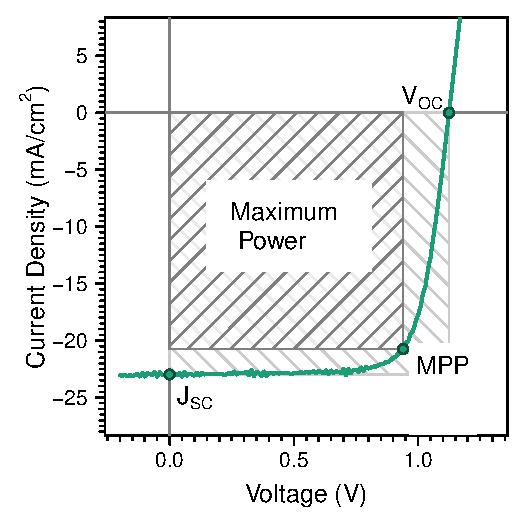
\includegraphics[width=0.6\textwidth]{iv_params/IV-revIVs.pdf}
			\mycaption[Solar cells parameters from current-voltage sweeps.]{A typical current-voltage sweep is represented.
				MPP stands for maximum power point, \gls{jsc} stands for \glsdesc{jsc}, \gls{voc} stands for \glsdesc{voc}.
				The ratio between the small and the large rectangles areas is the \gls{ff}.}\label{fig:iv_params}
		\end{SCfigure}

		\paragraph{\Glsentrydesc{voc}}
		\Gls{voc} parameter is defined as the voltage $V$ at which the current is zero while the solar cell device is illuminated and in steady state (positive by its own definition).

		\paragraph{\Glsentrydesc{jsc}}
		\Gls{jsc} parameter is defined as the unsigned value of the current density flowing in an external circuit short circuiting (zero resistance) the solar cell device's contacts while illuminated at 1~sun and in steady state.
		It is usually reported in current (milli Amperes) over active area (square centimetre) unit.

		\paragraph{Maximum power density}
		The maximum power density is defined as the unsigned minimum of electrical power density which can be obtained by $P(V) = J(V) \cdot V$.
		It is usually reported using power (Watt) over active area (square centimetre) unit.

		\paragraph{\Glsentrydesc{pce}}
		\Gls{pce} parameter is defined as the maximum power density over the illuminating power density, which at 1~sun AM 1.5G is defined to \SI{100}{\mW\per\square\cm}.
		It is usually reported as a percentage.

		\paragraph{\Glsentrydesc{ff}}\label{characterization_ff}
		\Gls{ff} parameter is defined as the ratio between \gls{pce} and the product of \gls{voc} and \gls{jsc}.
		This parameter does not have a physical meaning, but it represents how much the series and shunt resistances affect the device efficiency.
		It can be represented either as a fraction of unity or as a percentage.
		In \cref{fig:iv_params}, the \gls{ff} can be graphically obtained from the ratio of the areas of the two rectangles.

		\paragraph{Forward and reverse bias}
		Forward bias is a device condition where applied voltage is positive, reverse bias is the case where applied voltage is negative.

		\paragraph{Forward and reverse scan}\label{characterization_fwdrev}
		In current-voltage sweeps, a scan where the voltage is increasing over time is a forward scan, while a voltage variation in the opposite direction constitutes a reverse scan.

		\paragraph{Ideality factor}
		An ideality factor $n_|id|$ different from 1 describes deviations from the ideal photo-diode.
		The Shockley diode equation adapted for photogeneration becomes \cite{Calado2019}:
		\begin{equation} \label{eq:photodiode}
			J(V,\phi) = J_|ph|(\phi) - J_0\left[\exp(\frac{qV}{n_|id|k_|B|T})-1\right]
		\end{equation}
		where $J_|ph|$ is the total photo\hyp{}generated current (negative sign), $J_0$ is the dark diode saturation current (the current flowing in dark when applying a reverse bias, negative sign), $q$ is the elementary charge, $k_|B|$ is the Boltzmann constant, and $T$ is the temperature.
		If recombination losses at short circuit are negligible (which can be measured either with $\jsc$ \textsl{versus} $\phi$, see \cpageref{jsc-phi}, or with \acr{tpc}, see \cpageref{characterization_tpc}), the photo\hyp{}generated current can be approximated with the short circuit current $J_|ph|(\phi) \approx \jsc(\phi)$.
		Clearly the reported equation just offers a simplified model.
		For example, it can be improved adding the contribution from the series resistance $R_|s|$ and would become:
		\begin{equation}\label{eq:series_resistance}
			J = J_|ph|(\phi) - J_0\left[\exp(\frac{q(V+JR_|s|)}{n_|id|k_|B|T})-1\right]
		\end{equation}
		The function is now an implicit one, requiring numerical solving even for obtaining $\jsc$.
		Additionally, we can include the leakage current due to the internal shunt resistance $R_|sh|$ \cite{Nelson2003}:
		\begin{equation}
			J = J_|ph|(\phi) - J_0\left[\exp(\frac{q(V+JR_|s|)}{n_|id|k_|B|T})-1\right] + \frac{V+JR_|s|}{R_|sh|}
		\end{equation}

		\paragraph{Top and bottom of devices}
		The point of view of the manufacturer is used for defining the physical top and bottom of a device: the bottom is the glass substrate and the top is the last deposited layer.
		This is opposite with the usage of a solar cell in the real world and with most of the solar simulators (but not all of them
		%, for example Paios from Fluxim has an illumination from below, more convenient for contacting the electrodes without a samples holder
		\cite{Fluxim}).

	\subsection{Usage of Shadowing Mask}

		\begin{SCfigure}
			\centering
			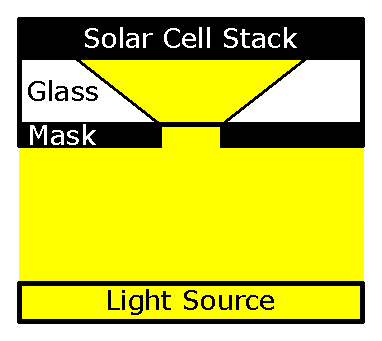
\includegraphics[width=0.35\textwidth]{shadowing_mask/shadowing_mask.pdf}
			\mycaption[Illuminated area after a shadowing mask.]{This schema is just for explaining the concept described in the text, its dimensions are not realistic.}\label{fig:shadowing_mask}
		\end{SCfigure}

		In literature is generally suggested to use a shadowing mask when measuring the solar cell devices in order to better define the illuminated area (\textsl{e.g.}\ in the obsolete \cite{Brinser2017} form by Nature publisher \cite{NatureResearch2017} or in \cite{Christians2015}).
		Our active area is just \SI{0.09}{\square\cm} so the mask aperture should be extremely small and its positioning troublesome.
		Additionally, the fact that the illumination reaches the mask from a wide angle (the illumination passes through spread lenses, whose size is not small compared to the lamp-cell distance) allows the light to spread through the substrate glass (\SI{2.2}{\mm} for our \gls{fto} substrates) illuminating a large area on the active layer, as represented in \cref{fig:shadowing_mask}.
		In our solar simulator a linear widening of 8~\% over \SI{2}{\mm} was estimated, this makes an illuminated area 16~\% larger than the mask aperture.
		Even if the total incident power is determined from the mask aperture, the incident intensity is not 1~sun any more, compromising the validity of the measurement.


	\subsection{Stability During the Measurement and Small\-/Large Perturbations}

		Most of the reported hybrid lead halide perovskite materials can show rather impressive changes in their structure on long time scales, for example due to ionic migration \cite{Calado2016}, degradation \cite{OKane2019}, and self-healing \cite{Ceratti2018}.
		This have to be taken into account for all the measurements techniques output which either takes too long time to be measured or employs large perturbations.

		\paragraph{Long lasting measurement}
		An example of the first case is the impedance spectroscopy where during the long lasting measurement various phenomena can occur, like: a slow current evolution due to perovskite well known hysteretic\index{hysteresis} behaviour prior to stabilisation; a degradation process changing the current; the heating of the device changing its properties.
		This slow current evolution can easily be misinterpreted for capacitive current \cite{Jacobs2018}, introduce artefacts like loops in the Nyquist plots \cite{Moia2019}, or even justify negative capacitance\index{negative capacitance} observations \cite{Knapp2015}.

		\paragraph{Large perturbations} \label{perturbation}
		Large perturbations regime means that the independent variable is changed by an amount large enough to cause the dependent variable to not adhere to the first term of its series expansion.
%		Let's take some examples.
		%		\paragraph{Large perturbations -- \acr{tpv}}
		For example, a too intense laser pulse in \acr{tpv} could change the voltage by a less\hyp{}than\hyp{}linear amount.
		In this case, the light pulse is not only probing the recombination, but it is adding some, so a large perturbation has to be avoided.
		This effect has been reported for \gls{dssc} in \authoryear{Barnes2013}.
		%		\paragraph{Large perturbations -- \gls{trpl}}
		Last example: in the \glsdesc{trpl} a laser pulse illuminates the otherwise unilluminated absorber layer.
		If mobile ions are present and if the absorber is in contact with other semiconductor layers generating a built-in voltage, this pulse induces some extent of ionic migration to a new profile \cite{Levine2018} (just consider that the ionic profile for a solar cell in dark and at \SI{1}{sun} is different, as the amount of electric field to screen is different).
		The extent of this migration will depend on the pulse intensity and duration.
		The fact that the relaxation time of the ionic migration (\si{\ms} to seconds for the ions \cite{Jacobs2018}) is usually much larger than the laser repetition rate (\si{\us} to \si{\ms} for typical \gls{trpl} lasers \cite{EdinburghInstruments}) implies that the ionic profile variation slowly "builds up" pulse after pulse.
		As the ionic profile affects the free charges concentration profile and non radiative surface recombination, and these in turn affect the radiative recombination, the measurements of \gls{trpl} in contacted perovskite layer have to be done with extreme care as they are expected to strongly depend on laser intensity and repetition rate.
		An example of hysteretic\index{hysteresis} behaviour observed with \gls{trpl} can be found in \authoryear{Motti2016} and elsewhere \cite{Chen2015,Chen2017}.
		This is not expected to be a problem for perovskite in contact just with isolating layers.
		%		This should also be considered when comparing lifetimes from different laser fluences \cite{Manser2014}.

\section{Current-Voltage Sweeps}

	\begin{SCfigure}%[!hbtp]%
	\centering
	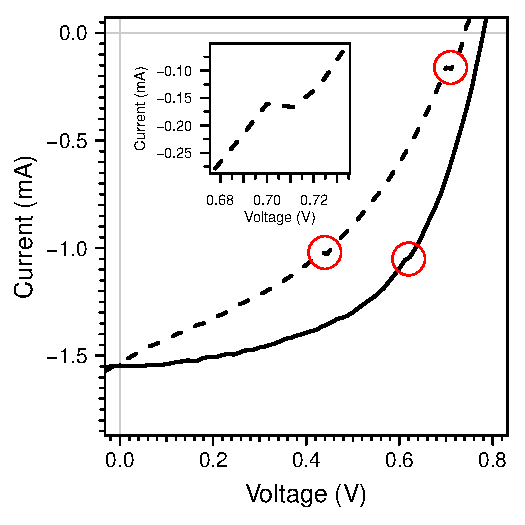
\includegraphics[width=0.6\textwidth]{autoscale/ig1-3-1-int4.pdf}
	\mycaption[Kinks in J-V sweep due to autoscale.]{A current\hyp{}voltage sweep of an hysteretic\index{hysteresis} perovskite solar cell with Keithley autoscale active.
		Both the forward (dashed) and the reverse (solid line) present small discontinuities around \SI{1}{\mA} and \SI{0.1}{\mA}.}\label{fig:autoscale}
\end{SCfigure}

	After calibrating the light intensity in the solar simulator (see \cpageref{solarsimulator}), the devices were exposed to the illumination at open circuit for some seconds in order to have a stabilised open circuit voltage.
	Then the curves were measured with the auto-measure function of the PyPV software which measures the reverse scan and then the forward scan (see \cpageref{automeasure}).

	\paragraph{Automatic scale}\label{autoscale}
	In literature one can easily find current\hyp{}voltage curves with discontinuities or "kinks" \cite{Li2016,Snaith2014,Zhang2015} like the one reported in \cref{fig:autoscale}, this is usually left unexplained.
	%	Some even lucubrate about the origin of these in perovskite solar cells.
	Disabling the auto-scale feature of the Keithley equipment the discontinuities disappear, so we can account these kinks to an hysteretic\index{hysteresis} effect happening during the instrumental scale change.
	%	It is likely due to the auto-scale feature of the Keithley equipment, as disabling this, the discontinuities disappear.



	\paragraph{Scan speed}\label{characterization_scanspeed}
	The used sweep speed is \SI{500}{\mV\per\s}, which was arbitrarily chosen for avoiding bumps leading to currents higher than \gls{jsc}, like the one in \cref{fig:iv_ugly} (seldom reported in literature, like in figure~S3 of \cite{Du2018} or for different speeds in \cite{CorreaBaena2015,Tress2015,Unger2014,Richardson2016} and simulated with drift-diffusion in \cite{Walter2018}).
	Our arbitrary choice allowed us to make fair comparisons between devices, but the absolute values should be considered as approximations.
	We wanted to underline that due to hysteresis\index{hysteresis} phenomena, no scan speed, direction, or precondition is the correct one.
	Rather, a static measurement or a \acr{mppt} should be used for obtaining a accurate and realistic result \cite{Zimmermann2016}.
	This comment regards also the so-called "hysteresis-free" perovskite solar cells, which can also present hysteretic\index{hysteresis} phenomena on different time\hyp{}scales \cite{Jacobs2018,Du2018} or temperatures \cite{Bryant2015}.
	
	\begin{SCfigure}%[!hbtp]%
	\centering
	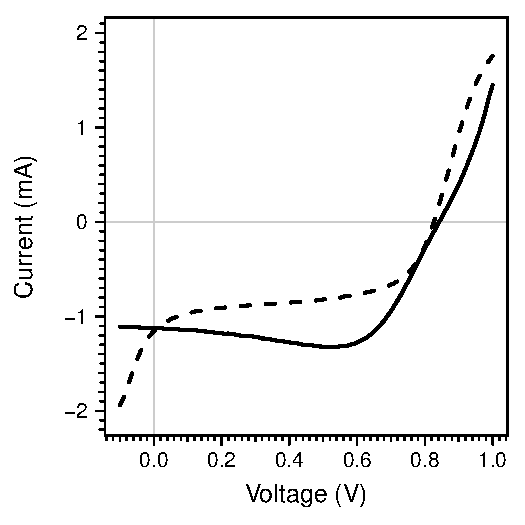
\includegraphics[width=0.6\textwidth]{iv_ugly/ig47-b32-int2-4.pdf}
	\mycaption[Hysteretic current-voltage scan.]{At the employed scan speed, the hysteresis\index{hysteresis} phenomena causes the reverse (solid line) scan to reach currents higher than the \gls{jsc}.}\label{fig:iv_ugly}
\end{SCfigure}

	\paragraph{Noise}
	The noise often observed in current-voltage sweeps at high scan speeds in this thesis is mainly caused by oscillations in the solar simulator illumination intensity, as an example see \cref{fig:iv_params}.
	For reducing the noise impact on the \gls{jsc} and \gls{voc} parameters extraction, these values were extracted \textsl{via} a parabolic fitting.

	\paragraph{Shunt and series resistances} \label{resistances}
	The shunt and series resistances can be evaluated by the current \textsl{versus} voltage derivative of a dark current-voltage sweep \cite{Pysch2007}.
	The former from the current values at voltages close to zero and the latter from the current at high-enough voltage.
	Perovskite solar cell hysteretic\index{hysteresis} behaviour can affect this measurement.
	An alternative could be to measure the stabilised current at a few voltage points: a couple of measurements close to zero voltage is enough for estimating the shunt resistance while two points at high voltages should be enough for estimating the series resistance.
	Still, the ionic profile would be different for the different applied voltages used for shunt resistance measurement, affecting the recombination barriers \cite{Moia2019,Pockett2017}.
	So a transient measurement similar to the one proposed for the ideality factor in \cite{Calado2019} and explained in \cpageref{transient_suns_voc} might be implemented for estimating the shunt resistance.
%	Instead, for series resistance the transient method should not be needed, as the large employed voltage employed voltages are always larger than the built-in voltage, the depletion\index{space charge layer} layers should be filled anyway and the transient method should not be required.
	Instead, for series resistance the transient method should not be needed, as the large employed voltage should be enough for flattening the ionic profile.
	The impact of these resistances on the \gls{pce} is paramount, as the \gls{ff} strongly depends both on series and on shunt resistances.

	\paragraph{Solar cells parameters extraction from sweeps}\label{characterization_hysteresis}
	For the devices studied in this thesis, the reported values of \gls{voc}, \gls{jsc}, \gls{pce} and \gls{ff} are extracted from a forward or reverse current-voltage sweep.
	This follows the tradition of solar cells reporting; but for hysteretic\index{hysteresis} devices, like perovskite solar cells, a static measurement should be preferred.
	%	\paragraph{Solar cells parameters extraction from sweeps -- \gls{pce}}
	For measuring the \gls{voc} or the \gls{jsc} a static measurement is experimentally straightforward.
	Instead, for the \gls{pce}, and by consequence the \gls{ff}, a proper measurement is made difficult due to the cell evolution over time (hysteresis).
	This evolution involves a drift of the maximum power point over the time, so a static measurement is suboptimal.
	A \acr{mppt} system has to be employed in order to track the voltage evolution of this point \cite{Zimmermann2016}.
	Such a system is not trivial, as the process of localisation of the maximum power point involves a varying applied voltage, which can trigger some hysteresis, some attempts to achieve a working \acr{mppt} system are described in \cpageref{software_mppt}.
	%	A proper  system needs to be bought or developed, see \cpageref{software_mppt} for thoughts about possible implementations.

	\paragraph{Stabilized or dynamic current-voltage sweeps}
	One very appealing alternative to current-voltage sweeps are the so-called "stabilised current-voltage sweeps", where at each voltage point a fixed stabilisation time is waited and the stabilised current is reported \cite{Unger2014, Christoforo2015, Christians2015}.
	An improvement of this technique is named "dynamic current-voltage sweeps", here the stabilisation step is of variable duration, until the current\hyp{}time derivative falls below a threshold (\textsl{e.g.}\ \SI{0.2}{\%\per\minute}) \cite{Dunbar2017,Dunbar2017a}.
	%	In this thesis, these techniques have not been used.


\section{\textit{V}\textsubscript{OC} and \textit{J}\textsubscript{SC} Dependence on Light Intensity}
	The solar simulator illumination intensity $\phi$ is reduced \textsl{via} neutral density filters with transmittance of 0.05, 0.12, 0.25, 0.51, 0.81 and 1 (no filter).
	The values of $\voc(\phi)$ and $\jsc(\phi)$ can be obtained from static measurements or from current-voltage sweeps.
	The static measurement of $\voc(\phi)$ at high light intensities is troublesome as it can easily damage the device.
	In this thesis, the used method is specified case by case.

	\subsection{\textit{J}\textsubscript{SC} \textsl{versus} $\phi$}\label{jsc-phi}
		The \gls{jsc} dependency on the light intensity $\phi$ is close to linear and can be fitted with a power law:
		\begin{equation} \label{eq:jsc-phi}
			\jsc \propto \phi^\alpha
		\end{equation}
		where $\alpha$ is a free fitting parameter. Its values usually range from 0.95 to 1.

		\paragraph{Interpretation}
		An $\alpha$ value lower than 1 indicates that not all the photo\hyp{}generated charges get extracted, neither at short circuit conditions.
		This can happen due to recombination processes (non-geminate ones, for geminate recombination see \cpageref{intro_geminate}) at short circuit \cite{Credgington2011} or of other factors limiting the charge collection.

	\subsection{\textit{V}\textsubscript{OC} \textsl{versus} $\phi$ and the Ideality Factor $n_|id|$}\label{characterization_ideality}
		Setting $J=0$, which corresponds to open circuit conditions, in \cref{eq:photodiode} (without considering the series resistance correction) we can obtain a relation between \gls{jsc} and \gls{voc}:
		\begin{equation}
			\jsc(\phi) = J_0\left[\exp(\frac{q\voc (\phi)}{n_|id|k_|B|T})-1\right]
		\end{equation}
		This equation can already be used for obtaining the $n_|id|$ and $J_0$ values fitting the \gls{jsc} and \gls{voc} measured at different light intensities $\phi$ (also varying the temperature could be used for fitting the values, but it was not done during this thesis \cite{Tvingstedt2016}).
		Solving for \gls{voc} we obtain:
		\begin{equation}\voc = \frac{n_|id|k_|B|T}{q}\cdot\ln\left(\frac{\jsc}{J_0} + 1\right)\end{equation}
		Considering that the saturation current $J_0$ (current in dark under reverse bias) is much smaller than $\jsc$ for the light intensities we usually employ (down to \SI{0.05}{suns}), we can approximate to:
		\begin{equation}
			\voc \approx u_1 + \frac{n_|id|k_|B|T}{q}\cdot\ln(\jsc)
		\end{equation}
		where $u_1$ is a useless constant.
		Then if the $\alpha$ value is close enough to~1, we can use \cref{eq:jsc-phi} and further approximate for plotting against light intensity $\phi$:
		\begin{equation}\label{eq:voc_vs_phi}
			\voc (\phi) \approx u_2 + \frac{n_|id|k_|B|T}{q}\cdot\ln(\phi)
		\end{equation}
		This is the equation we commonly employ for fitting and obtaining an ideality factor value \cite{Nelson2003} as it conveniently uses a zero current measurement (\gls{voc}) so that series resistance can be completely ignored \cite{Kirchartz2012}.
		%		In some cases this latest expression is used as ideality factor definition 
		The shunt resistance will still affect the measurement \cite{Tvingstedt2017}.
		The so-obtained ideality factor $n_|id|$ is usually from 1 to 2.
		A light bias/illumination dependent ideality factor can also be measured either from a current-voltage sweeps in dark (which would be influenced by hysteretic\index{hysteresis} behaviour) or from a derivative form of \cref{eq:voc_vs_phi} \cite{Calado2019}:
		\begin{equation}
			n_|id|(\phi_0) = \frac{q}{k_|B|T} \eval{\dv{V_|OC|}{\ln(\phi)}}_{\phi=\phi_0}
		\end{equation}
		%		The latter method has not been tested in this thesis as it would be affected by hysteresis.

		\begin{figure}
			\makebox[\textwidth][c]{
			\parbox{1.1\textwidth}{
			\centering
			\begin{subfigure}[t]{0.5\textwidth}
				\includegraphics[width=1\textwidth]{vapp_builtin/levels_and_ions_dark.pdf}
				\subcaption{Dark, $V=0$}\label{fig:vapp_builtin-levels_and_ions_dark}
			\end{subfigure}
			\qquad
			\begin{subfigure}[t]{0.5\textwidth}
				\includegraphics[width=1\textwidth]{vapp_builtin/levels_and_ions_dark_vapp_builtin.pdf}
				\subcaption{Dark, $V=V_|BI|$}\label{fig:vapp_builtin-levels_and_ions_dark_vapp_builtin}
			\end{subfigure}
			\mycaption[Simulated effect on the ionic profile of the application of a voltage equal to the built-in voltage.]{A $p$(\SI{200}{\nm})--$i$(\SI{500}{\nm})--$n$(\SI{200}{\nm}) homojunction device is simulated, above the energy levels are reported and below the ionic density profile is reported. In (\textbf{a}) the device is at equilibrium in dark. In (\textbf{b}) the device is in steady state in dark with an applied voltage equal to the built-in voltage $qV=qV_|BI| = \bar\mu^{\mathrm{cathode}} - \bar\mu^{\mathrm{anode}} \approx \bar\mu_|CB|^{\mathrm{ETM}} - \bar\mu_|VB|^{\mathrm{HTM}}$.}\label{fig:vapp_builtin}
			}
			}
		\end{figure}

		\paragraph{Transient Suns-\textit{V}\textsubscript{OC}}\label{transient_suns_voc}
		A critical analysis of these methods and the proposal of a new "Transient Suns-\gls{voc}" method can be found in \authoryear{Calado2019}.
		In their work the authors propose to precondition the device in dark at an applied voltage bias roughly equal to the built-in voltage.
		After this stabilisation step the needed measurement conditions are applied (illumination is switched on and open circuit conditions are set) and the interesting quantity measured within a few milliseconds.
		The preconditioning step can increase the filling of the depletion\index{space charge layer} layers in the contacts, which makes the ionic accumulation at the interface vanish through diffusion, or at least decrease.
		This is illustrated in \cref{fig:vapp_builtin} where a simulation of an homojunction device is reported.
		While the ionic profile is flat through the perovskite layer, the electronic properties of the cell can be studied using the theory from \gls{osc} \textsl{i.e.}\ without the influence of ionic accumulation.
		Please notice that in the real case of a heterojunction device, where the two selective contacts have different band gaps, this flattening of the ionic profile could be impossible.

		\paragraph{Interpretation} %\The \gls{voc} dependency on the light intensity $\phi$ can be fitted with a natural logarithmic dependence obtaining the ideality factor $m$. 
		\authoryear{Pockett2015} measured ideality factors of planar perovskite solar cells \textsl{via} stabilised \gls{voc} obtaining, for some cases, values as high as 5.
		Also in organic \cite{Kirchartz2011,Kirchartz2012} and silicon solar cells \cite{Breitenstein2006} ideality factors greater than 2 has been observed and explained.
		According to \authoryear{Calado2019} and \authoryear{Kirchartz2012}, the ideality factor, once obtained in the correct way, is 1 when studying most of the recombination types and 2 for mid-gap trap mediated recombination in regions where the electrons and holes concentrations are similar, $n \approx p$.

		\FloatBarrier
		\newpage
\section{Charge Extraction (\glsentryshort{ce})}\label{characterization_ce}

	\begin{SCfigure}
		\centering
		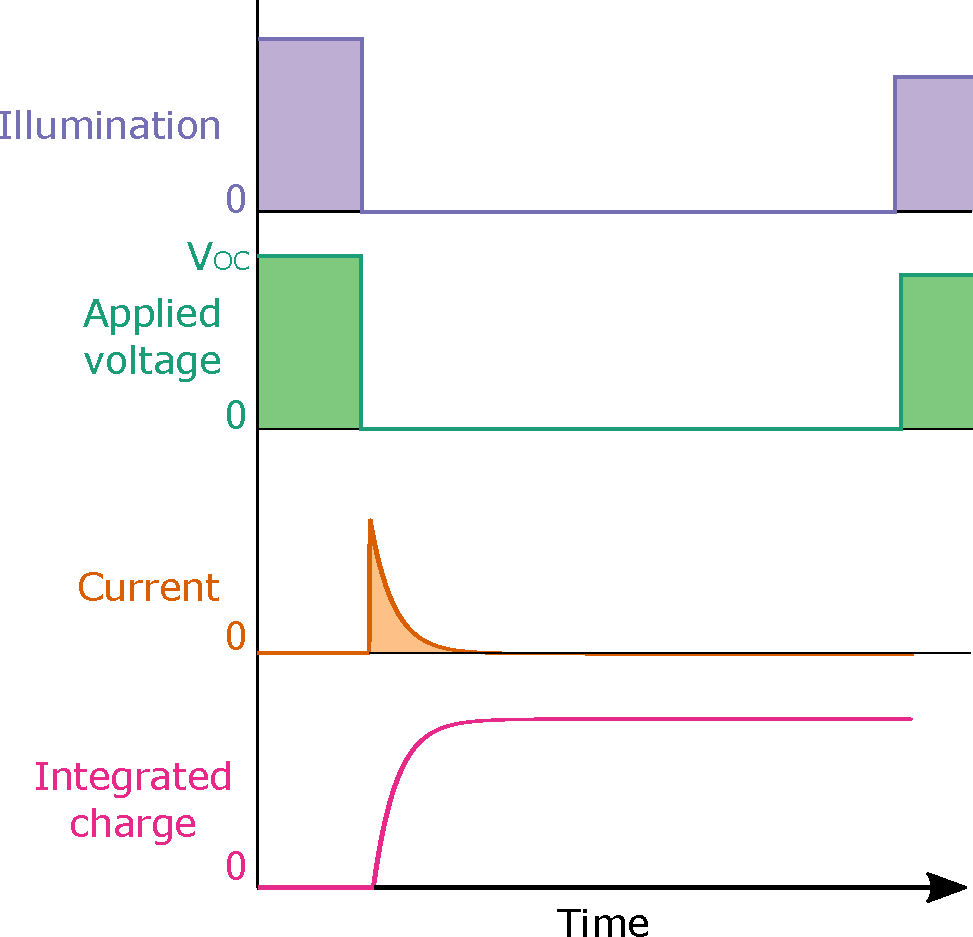
\includegraphics[width=0.65\textwidth]{ce_scheme/ce_scheme.pdf}
		\mycaption[Scheme of CE experiment.]{
			A device is illuminated in open circuit conditions, then simultaneously the illumination is switched off and the circuit is closed through a small resistance. The current flowing gets integrated to obtain the extracted charge. Then the illumination is switched on at a different intensity and the measurement is repeated.}\label{fig:ce_scheme}
	\end{SCfigure}


	\paragraph{Concept}
	The charge extraction experiment has been designed to quantify the free charges available in a device \cite{Duffy2000,Barnes2011}.
	It works \textsl{via} the sudden extraction of the free charges in a solar cell illuminated at open circuit conditions.
	%	After stabilisation of a device at a light intensity and an applied voltage (in our case always at \gls{voc}), the illumination is switched off and the electrodes of the device are short circuited.
	%	The transient current flowing through the short circuiting circuit can be measured and integrated to estimate the available charge.
	The measured charge has to be considered as a lower bound to the actually present excess charge, as part of it could recombine inside the device during the extraction time \cite{ORegan2005}.
	Performing this experiment at various light intensities, we can obtain a charge density \textsl{versus} light bias relationship.

	\paragraph{Procedure}
	As represented in \cref{fig:ce_scheme}, the device is kept under constant illumination by a white \gls{led} at open circuit conditions until stabilisation is reached.
	After stabilisation, the illumination is suddenly switched off and, at the exactly same moment, the device is short circuited through a small and known resistance (\SI{50}{\ohm}).
	In the first microseconds, most of the free charge flows through the resistor generating a current and a voltage drop across it.
	An oscilloscope in parallel to this resistance measures the transient voltage.
	%This potential drop can be converted to current using the Ohm's law, which, integrated over time, gives the amount of extracted charge.
	The current flowing at any moment can be obtained from the measured voltage \textsl{via} Ohm's law: $J=V/R$ where $R$ is \SI{50}{\ohm}.
	This transient current can be integrated over time to obtain the extracted charge.
	Then the light intensity is decreased and the experiment is repeated, from 1~sun down to dark (in dark no signal should be observed).
	A single decay is measured for each illumination point, over a few tens of different illumination intensities.
	The results are plotted as charge density \textsl{versus} light bias.
	%, indeed some residual charge can usually be seen, the reason of this could be ionic profile updating or an insufficient darkness
	The equipment switching off the illumination and setting the short circuiting includes two transistors (circuit designed and built by Dr.\ Javier Pérez Hernández) and gets activated by a square voltage pulse from a pulse generator, the pulse is, at least, as long as the measurement window.
	From my experience, I recommend to use a short dark period in order to save time for the following stabilisation step.
	1~sun equivalent illumination is defined as the illumination at which a silicon photodiode gives the same \gls{jsc} as under calibrated 1~sun from the solar simulator.
	The \gls{led}-solar spectral mismatch affects slightly the measurement, but in no case a \gls{pce} is reported from any \gls{led}-illuminated experiment.

	\paragraph{Noise sources} \label{ce_noise}
	The lack of complete stabilisation of the device before the extraction of charge can introduce both an error in the measured \gls{voc} and in the extracted charge.
	Regarding the \gls{voc}, in perovskite solar cells it not only depends on the illumination intensity, but it also evolves slowly until the stabilisation at the steady state value, so a well defined stabilisation procedure is key for achieving reproducibility in \acr{ce} experiments.
	Regarding the extracted charge, the ionic profile can influence the amount of accumulated charge, as shown for two extreme cases of presence/absence of ionic charges in \cref{fig:ce_full_dd}, so a reproducible procedure for device stabilisation will also improve the reproducibility of the integrated current amount.
	Additionally, the measurement equipment introduces some electronic noise whose effect can be mitigated through data post-processing.

	\begin{figure}
		\makebox[\textwidth][c]{
			\parbox{1.1\textwidth}{
				\centering
				\begin{subfigure}[t]{1\textwidth}
					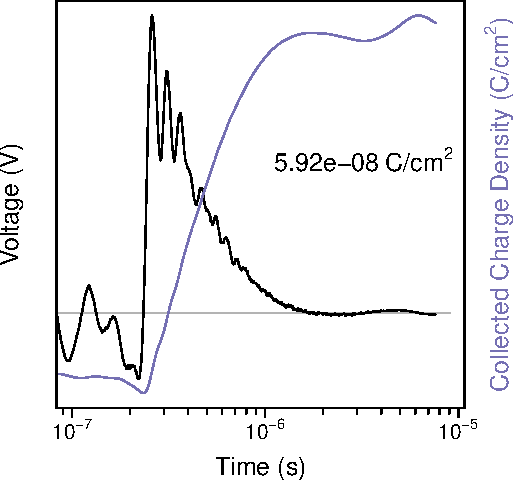
\includegraphics[width=0.4\textwidth]{{ce_noise/normal-CE_ig104-1566-4_Voc_0.911mV-crop}.pdf}
					\qquad
					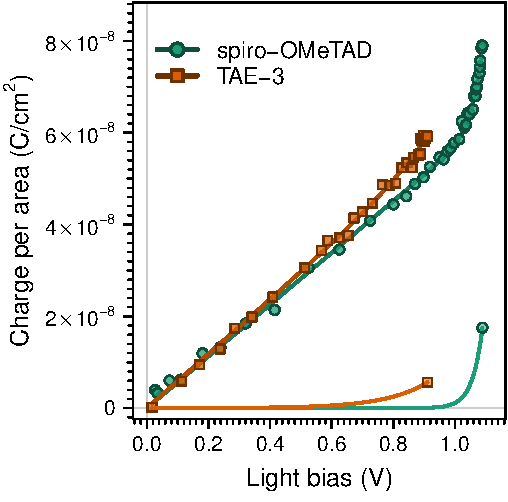
\includegraphics[width=0.39\textwidth]{ce_noise/normal-spiro_vs_TAEs-CEs-crop.pdf}
					\subcaption{Direct integration of raw data}\label{fig:ce_noise-normal}
				\end{subfigure}
%				\bigskip

				\begin{subfigure}[t]{1\textwidth}
					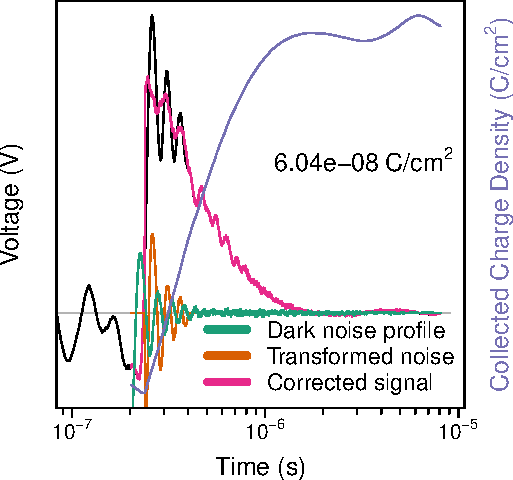
\includegraphics[width=0.4\textwidth]{{ce_noise/subtractDark-CE_ig104-1566-4_Voc_0.911mV-crop}.pdf}
					\qquad
					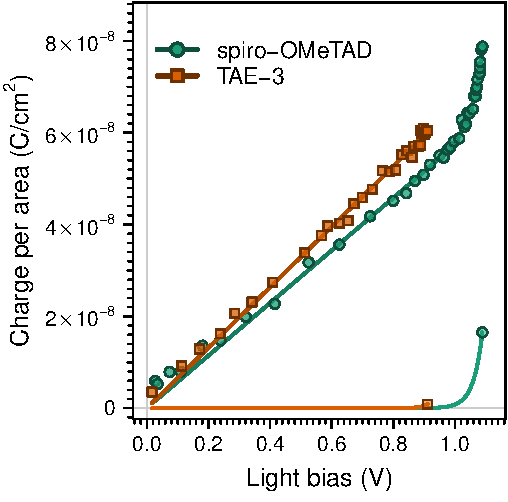
\includegraphics[width=0.39\textwidth]{ce_noise/subtractDark-spiro_vs_TAEs-CEs-crop.pdf}
					\subcaption{Subtraction of transformed noise profile}\label{fig:ce_noise-subtractDark}
				\end{subfigure}
%				\bigskip

				\begin{subfigure}[t]{1\textwidth}
					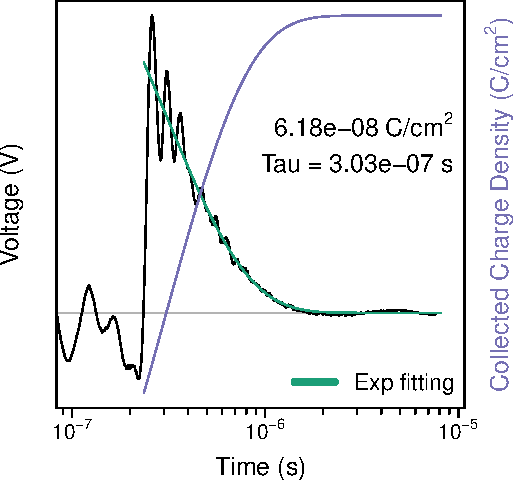
\includegraphics[width=0.4\textwidth]{{ce_noise/integrateExp-CE_ig104-1566-4_Voc_0.911mV-crop}.pdf}
					\qquad
					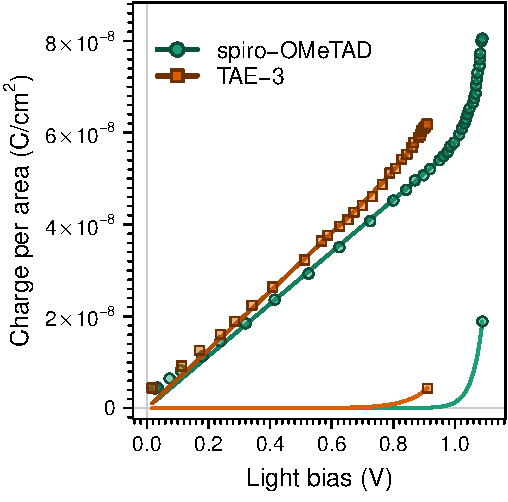
\includegraphics[width=0.39\textwidth]{ce_noise/integrateExp-spiro_vs_TAEs-CEs-crop.pdf}
					\subcaption{Integration of an exponential fitting}\label{fig:ce_noise-integrateExp}
				\end{subfigure}

				\mycaption[Strategies for reducing the instrumental noise in a single \glsentryshort{ce} integration.]{
					On the left, single \acr{ce} decays from a \gls{fto}\-/\ch{d-TiO2}\-/\gls{csfamapbibr}\-/\gls{tae3}\-/\ch{Au} device \cite{Gelmetti2019} is integrated without noise reduction in (\textbf{a}), adapting the noise profile from the dark measurement and subtracting it in (\textbf{b}), or fitting the decay and integrating the fit in (\textbf{c}).
					On the right, the charge \textsl{versus} voltage trends obtained applying the respective noise reduction methods.}\label{fig:ce_noise}
			}
		}
	\end{figure}

	\paragraph{Reduction of instrumental noise}\label{r_ce_noise}
	Most of the observed short\hyp{}time noise (\SI{< 5E-7}{\s}) observable in \cref{fig:ce_noise-normal} is related to the opening and closing of the transistor switches included in the home\hyp{}made circuit.
	The characteristic frequencies of the observed noise are not small compared to the measurement window, so its time\hyp{}integral does not necessarily sum to zero.
	In order to reduce its impact, various approaches have been tested and here described.
	The noise can be ignored in some cases, but it is a problem if the charge \textsl{versus} light bias (\gls{voc} generated at a given illumination intensity) profile, reported on the right hand column of \cref{fig:ce_noise}, has to be studied in detail, as in \cref{ch:tae}.
	In the mentioned case, just the exponential part of its linear plus exponential behaviour, reported in the bottom of each right hand figure, was of interest and it is evident that the employed noise\hyp{}reduction method influences it heavily.

	\paragraph{Reduction of instrumental noise -- subtraction of dark noise}\label{characterization_subtractDark}
	Annoyingly, the noise profile is characteristic of the cell and of the circuitry, so a simple average over many decays does not help in cancelling it.
	Based on this consideration, we tried to subtract a pure noise profile as obtained from a dark measurement (without any light bias).
	The operation was made more difficult by the slight variations of the noise profile with the light bias.
	A data\hyp{}to\hyp{}morphed\hyp{}noise fit was implemented where the $f(t)$ noise profile was transformed with: $t'= u_3 + u_4 \cdot t + u_5 \cdot t^2$ and $f'(t') = u_6 \cdot f(t') + u_7 \cdot t' \cdot f(t') + u_8 \cdot e^{-t'/u_9}$ where $u_{3-9}$ are constrained fit variables.
	Then $u_6$ was set to zero and the resulting profile was subtracted from the data and the result integrated.
	As can be seen in \cref{fig:ce_noise-subtractDark}, this technique is working for most of the cases but it can fail if the noise profile changes in a more complex fashion.

	\paragraph{Reduction of instrumental noise -- integration of a fitting}\label{characterization_integrateExp}
	Finally the decays were fitted with a bi\hyp{}exponential formula (sum of two exponential) or, if the bi\hyp{}exponential fitting was not converging, by a simple exponential and the integral of this fit was used.
	In both cases a robust fitting routine was employed \cite{Maechler2018}.
	
\begin{figure}
	\makebox[\textwidth][c]{
		\parbox{1.1\textwidth}{
			\centering
			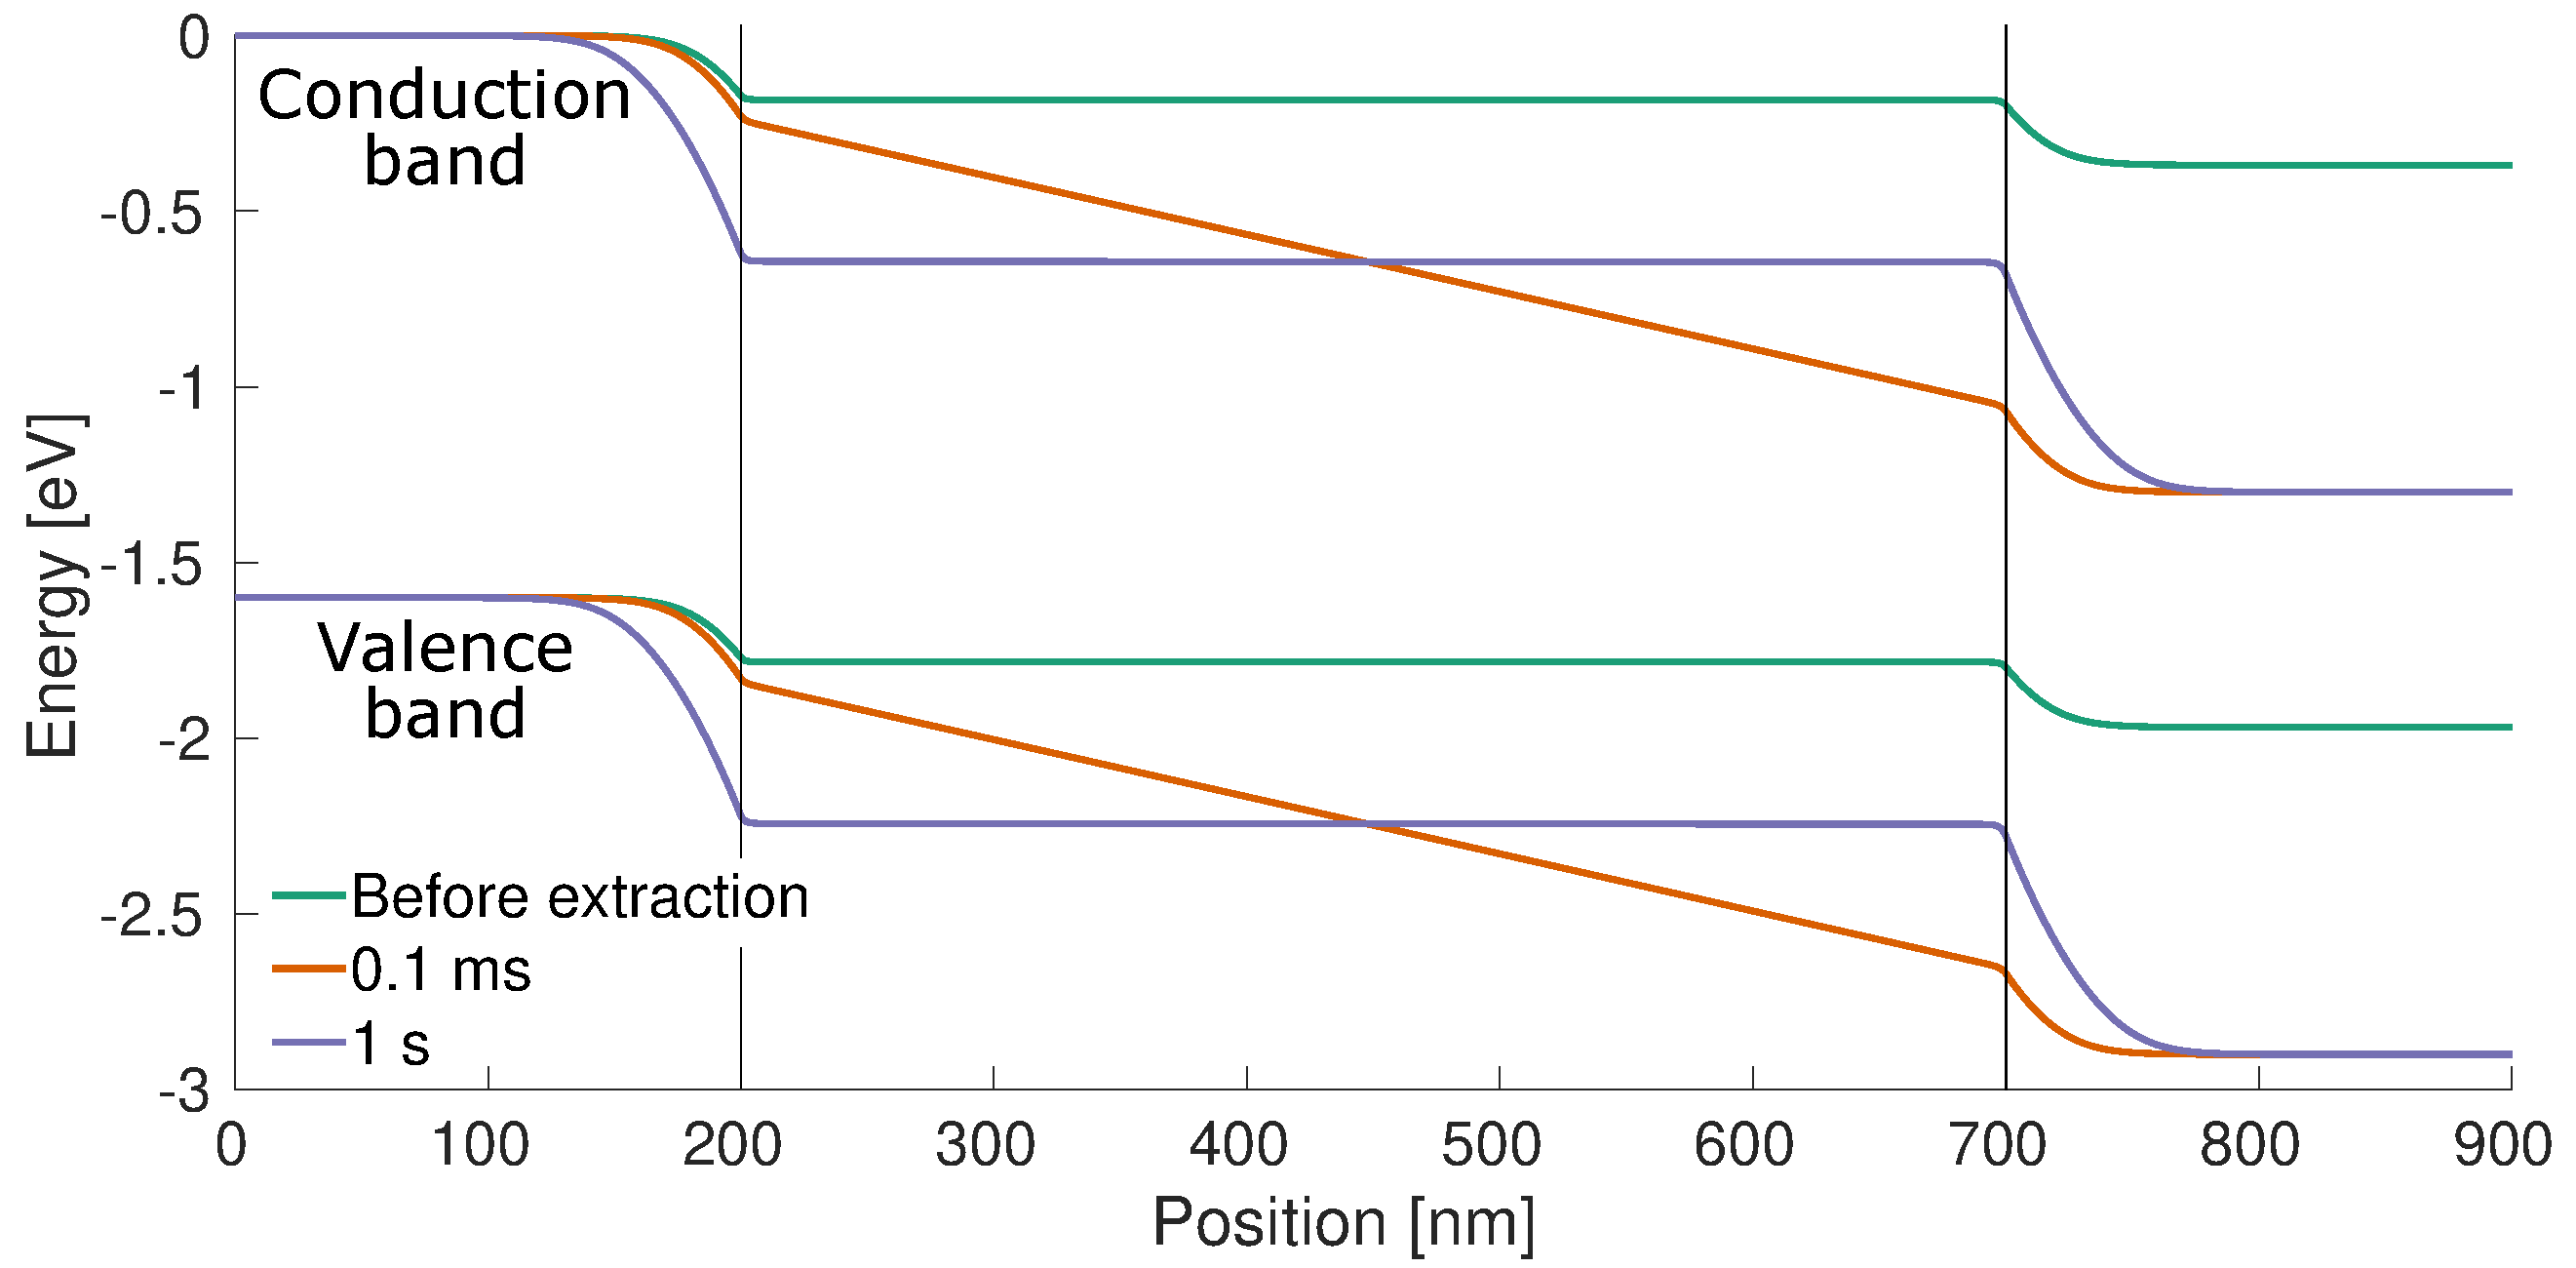
\includegraphics[width=0.9\textwidth]{ce_single_dd_levels_dynamic/ce_levels_corrected.pdf}
			\mycaption[Evolution of energy levels during CE.]{
				A $p$(\SI{200}{\nm})--$i$(\SI{500}{\nm})--$n$(\SI{200}{\nm}) device is simulated and the energy levels evolution during a \acr{ce} experiment are shown.
				At the beginning, the device is stabilised at open circuit conditions under \SI{1}{sun} illumination, represented by the green lines.
				Then the illumination is switched off and the device is brought to short circuit.
				After \SI{1e-4}{\s}, the electronic charges have been extracted, leaving an electric field in the bulk of the perovskite layer.
				Subsequently, at long times (\SI{1}{\s}) the ions move for screening the mentioned electric field.
				\Gls{ce} simulation routines explained in \cpageref{dd_ce}.
			}\label{fig:ce_levels_corrected}
	}}
\end{figure}

	\paragraph{Specific limitations for perovskite solar cells} \label{ce_limitations_perovskite}
	When measuring the \acr{ce} of a perovskite solar cell, additionally to the aforementioned limitations, one should also consider that the ionic profile update (from $V=\voc$ to $V=0$) causes a displacement current\index{displacement current}, as described in \cpageref{intro_displacement_current}.
	A simulation with Driftfusion has been performed for an homojunction device, the evolution of the energy levels is shown in \cref{fig:ce_levels_corrected} and two well distinct processes are observed with the extraction of free charges over short times and the rearrangement of ionic defects over long times.
	In \cref{fig:ce_single_dd-ions}, we can see the fast extraction of the free charges in the short time region.
	Zooming in the long times region, shown in \cref{fig:ce_single_dd-ions_zoom}, we can see that a very weak but long lasting current appears and gives a relevant contribution to the integrated charge, this is caused by the slow ionic profile change (and the related displacement current\index{displacement current}).
	This will happen on very large time scales and it will not affect the short measurements used for the free charges estimation, so it is rarely reported \cite{ORegan2015b}.
	The charge measured in the external circuit due to the ionic displacement current\index{displacement current} could be underestimated as the free charges rearrangements can also occur through the perovskite layer rather than through the external circuit.

\begin{figure}
	\makebox[\textwidth][c]{
		\parbox{1.1\textwidth}{
			\centering
			\begin{subfigure}[t]{0.5\textwidth}
				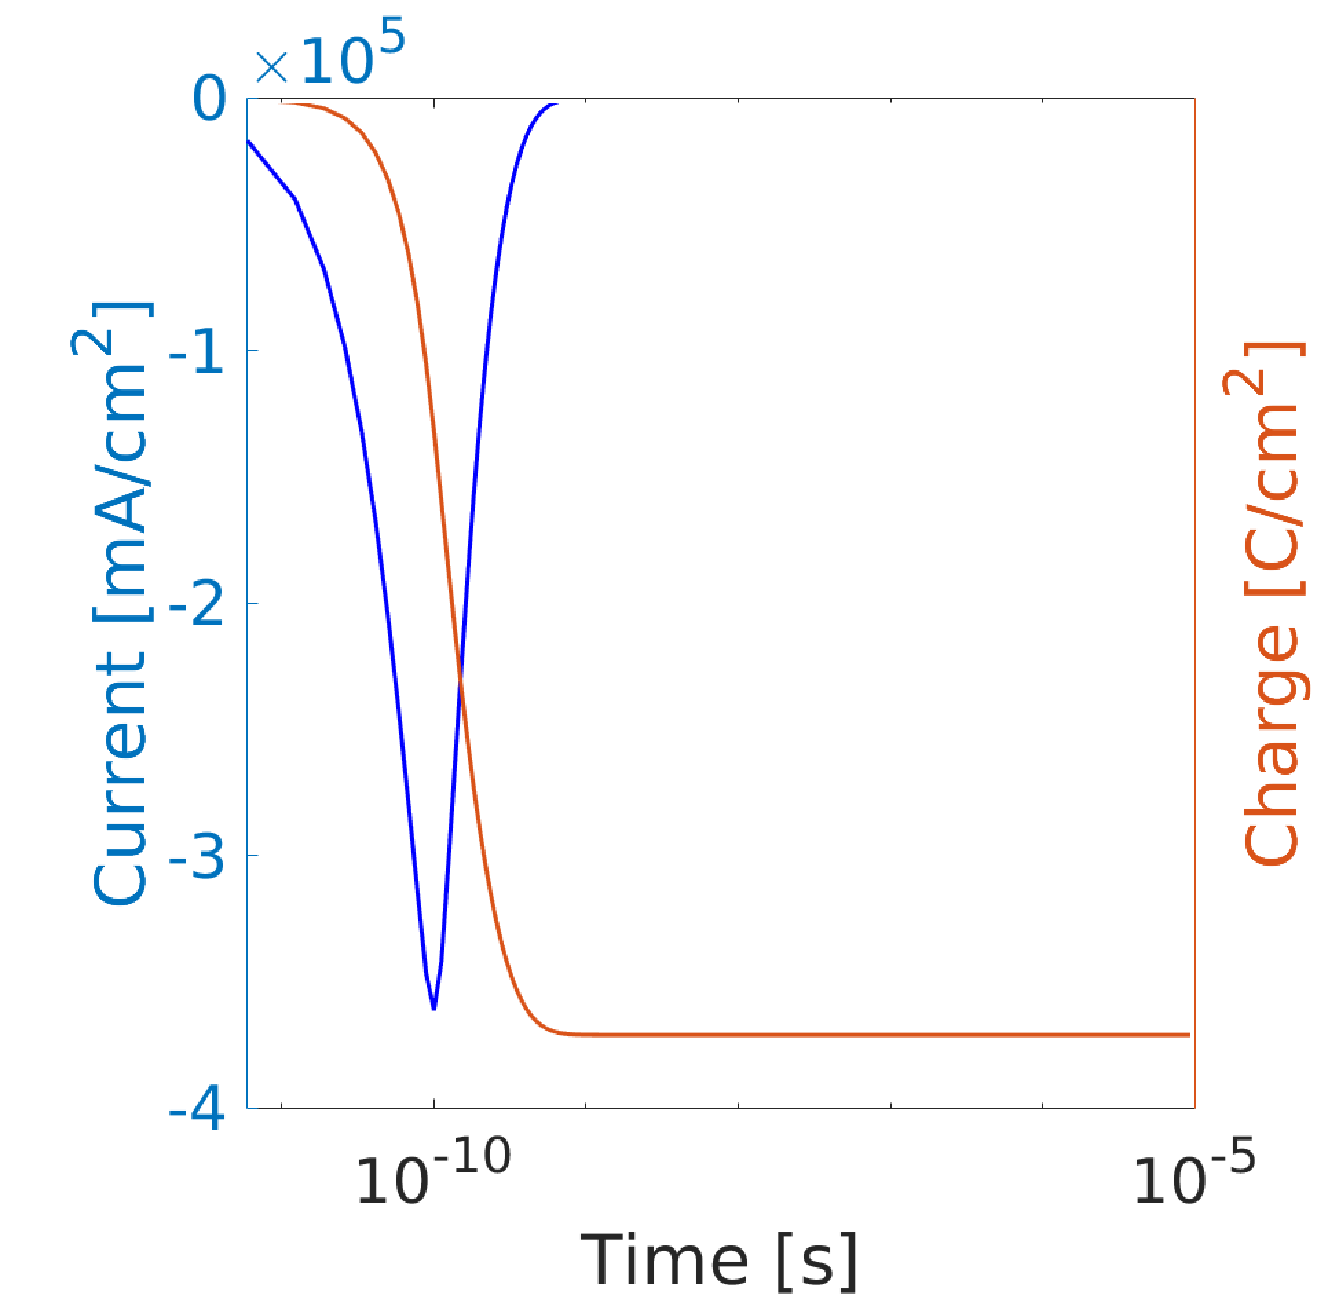
\includegraphics[width=1\textwidth]{ce_single_dd/ce_single_dd-noions.pdf}
				\subcaption{Without mobile ions}\label{fig:ce_single_dd-noions}
			\end{subfigure}
			\bigskip
			
			\begin{subfigure}[t]{0.5\textwidth}
				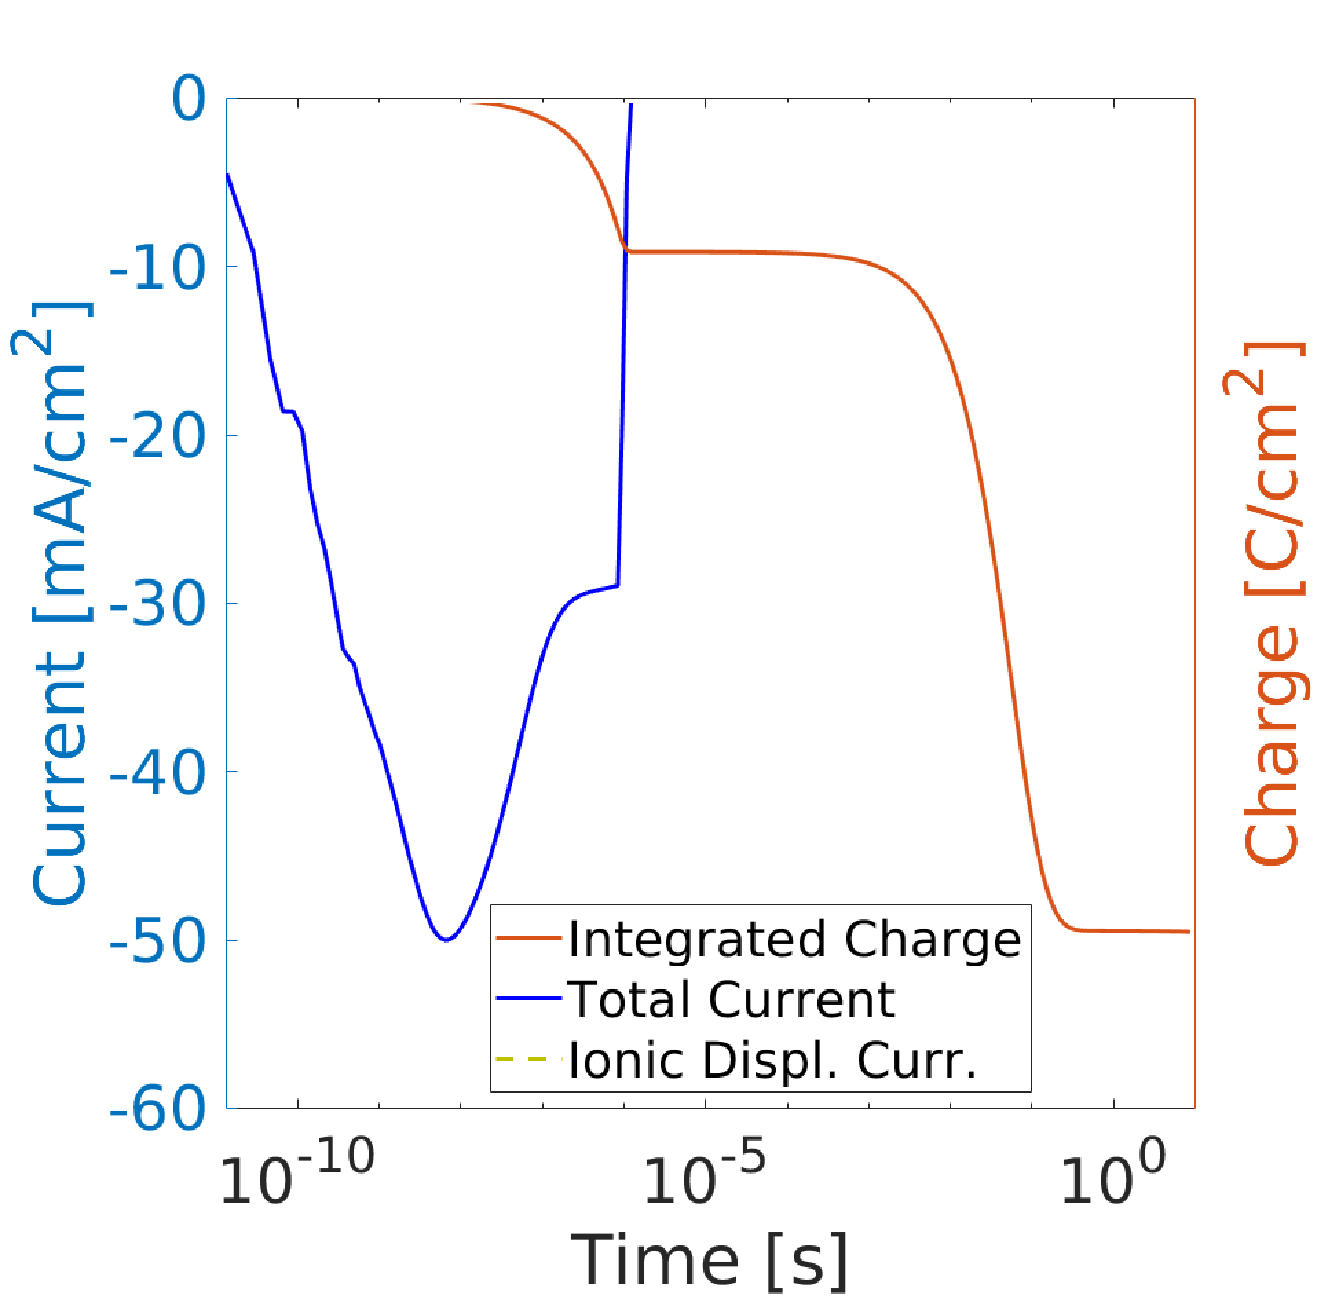
\includegraphics[width=1\textwidth]{ce_single_dd/ce_single_dd-ions.pdf}
				\subcaption{With mobile ions}\label{fig:ce_single_dd-ions}
			\end{subfigure}
			\qquad
			\begin{subfigure}[t]{0.5\textwidth}
				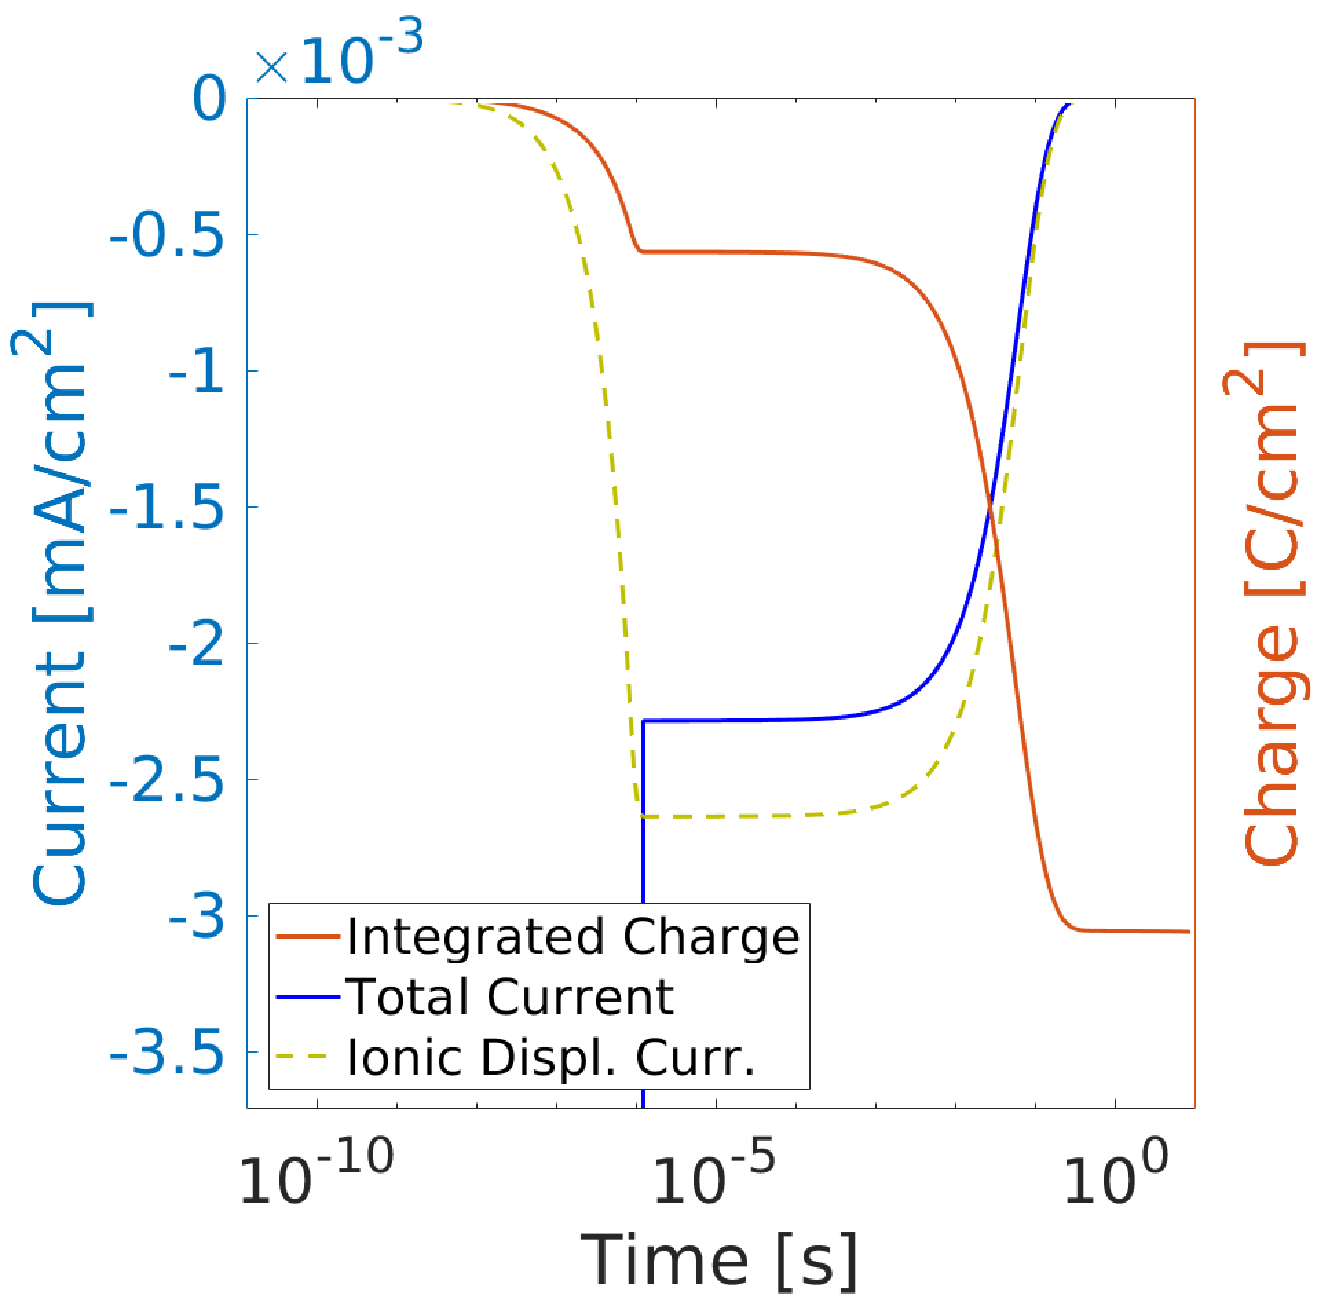
\includegraphics[width=1\textwidth]{ce_single_dd/ce_single_dd-ions_zoom.pdf}
				\subcaption{With mobile ions, magnified current density axis}\label{fig:ce_single_dd-ions_zoom}
			\end{subfigure}
			
			\mycaption[Simulation of a single CE current profiles without or with mobile ions.]{
				The current \textsl{versus} time profile of a \acr{ce} simulated experiment is shown on the left axis just for the 1~sun illumination intensity.
				On the right axis the cumulative integration of the extracted charge.
				Clearly, the extraction is unrealistically quick as the resistance included in a real \acr{ce} experiment was not included in the simulation.
				In (\textbf{a}) the measurement of a device without mobile ions is shown, we can observe just one current peak contributing to the integrated charge; in (\textbf{b}) the presence of the mobile ions introduces a long\hyp{}times contribution to the extracted charge, the current causing this is very weak and long lasting, it can be better observed in the magnification in (\textbf{c}).
				\Gls{ce} simulation routines explained in \cpageref{dd_ce}.
		}\label{fig:ce_single_dd}
		}
	}
\end{figure}


	\subsection{Interpretation of CE Single Decays}

		\paragraph{Charge extracted}
		The integrated charge is assumed to include the excess free charges in the valence and conduction bands.
		With \emph{excess} we refer to the difference between the charge concentration in the conditions of interest and the stabilised dark condition.
		For a non perfectly crystalline material, localised shallow traps constituted by the tails of the valence and conduction bands density of states inside of the so\hyp{}called mobility gap \cite{Pieters2009} are not negligible and should also contribute to the extracted charge amount \cite{Kirchartz2012,Du2018}.
		On the contrary, charges trapped in deep traps contributing to SRH trap mediated recombination, with energies far from the band edges, should not be possible to extract in a \acr{ce} experiment.

		\paragraph{\Glsentryshort{ce} time constant}\label{ce_time}
		The free charges extraction time is related to the RC time of the \SI{50}{\ohm} resistor and the capacitance of the solar cell device.
		We can see in \cref{fig:chargeExtraction_RCtime} a weak covariance (Pearson correlation coefficient of 0.3) between the RC time obtained extrapolating the dark capacitance from \acr{dc} (which is the geometric capacitance\index{geometric capacitance}) and the extraction time (as obtained by an exponential fitting to a single \acr{ce} current decay) at low light intensity (enough for having a signal but far from 1~sun light intensity).
		At higher light intensities, the correlation is weaker as the capacitance is less defined as the cell is in a transition between illuminated (high capacitance) and dark (low capacitance) status.
		Anyway, the extraction time does not change much between low light intensity and 1~sun with an increase from \SIrange{1.1}{2.4}{times} (first and third quartile).
		More discussion on this topic can be found on \authoryear{Montcada2018}.

		\begin{SCfigure}%[!hbtp]%
			\centering
			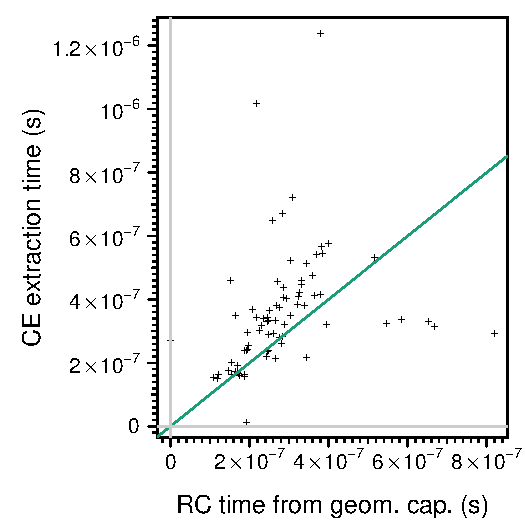
\includegraphics[width=0.45\textwidth]{chargeExtraction_RCtime/CEaBitOfSunExpTime_vs_RCdarkTime.pdf}
			\mycaption[Charge extraction time is related to a RC time.]{
				Covariance of \acr{ce} extraction time at low light intensity \textsl{versus} the expected time from geometric capacitance\index{geometric capacitance} (as obtained from dark \acr{dc}).
				Each point is a different device for a total of 78 devices, many different structures studied during my PhD are represented.
				The green line indicates the 1 to 1 relationship.}\label{fig:chargeExtraction_RCtime}
		\end{SCfigure}

		\paragraph{\Glsentryshort{ce} time constant and \glsentryshort{tpv} time constant -- Corrections}\label{characterization_ce_correction}
		During this time, and depending on its location in the device stack, some free charges can recombine.
		One could argue that a \acr{ce} measurement is valid only if the extraction is faster than the recombination time as measured \textsl{via} \acr{tpv} \cite{Ryan2017a} or that the extracted charge should be corrected considering the recombination \cite{Credgington2011,Credgington2014}.
		Considering the charges accumulated in the depletion\index{space charge layer} layers in the selective contacts, these will flow to the electrodes without crossing the perovskite/selective contacts interfaces, where has been reported that most of the recombination occurs \cite{Barnea-Nehoshtan2014,Stolterfoht2018a,Stolterfoht2018}.
		So this part of the extracted charge, distinguishable as the linear part of the charge \textsl{versus} voltage plot, as represented on the right column of \cref{fig:ce_noise} should not be corrected.
		Instead, regarding the charge accumulating in the perovskite layer, which we assume can be assigned to a chemical capacitance\index{chemical capacitance} and can be recognized as the exponential part on the right column of \cref{fig:ce_noise}, it may be that a correction \cite{Shuttle2008a,Shuttle2008b} is needed, but this has not be attempted in this thesis.

		\paragraph{\Glsentryshort{ce} time constant and \glsentryshort{tpv} time constant -- Correlation?}
		Some covariance (Pearson correlation coefficient of~0.4) can be observed in \cref{fig:ce_1sun_time_vs_tpv_1sun_time} between the \acr{ce} and the \acr{tpv} time constants at 1 sun illumination.
		This is unexpected and weird as the two times change with very different trends with light bias (when changing the preconditioning light intensity, \acr{ce} extraction time changes just slightly while \acr{tpv} decay time varies over various orders of magnitude).
		In case a stronger proof of correlation is found, this could indicate that both processes, even if not of the same nature, are limited by the same diffusion process, for example the migration of free charges from all the absorber to the absorber/contacts interfaces.

		\begin{SCfigure}%[!hbtp]%
			\centering
			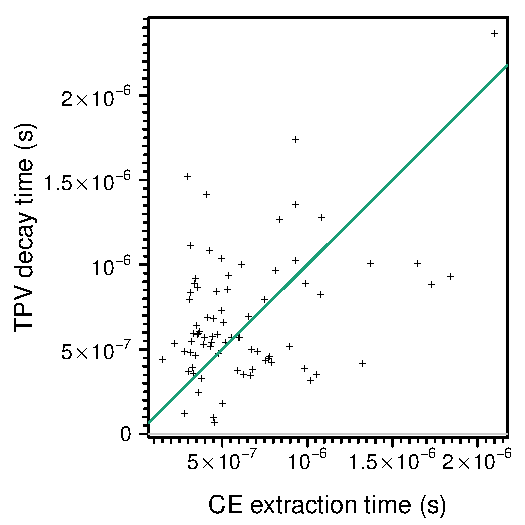
\includegraphics[width=0.45\textwidth]{ce_1sun_time_vs_tpv_1sun_time/ce_1sun_time_vs_tpv_1sun_time.pdf}
			\mycaption[Comparison between \glsentryshort{ce} and \glsentryshort{tpv} exponential decay times.]{
				Covariance of \acr{ce} extraction time at 1~sun light intensity \textsl{versus} the \acr{tpv} mono\hyp{}exponential decay time at 1~sun light intensity.
				Each point is a different device for a total of 79 devices, including many different structures.
				The green line indicates the 1 to 1 relationship.}\label{fig:ce_1sun_time_vs_tpv_1sun_time}
		\end{SCfigure}

	\subsection{Interpretation of CE \textsl{versus} Light Bias Without Mobile Ions}

		\paragraph{Exponential part and chemical capacitance\index{chemical capacitance} in \glsentryshort{osc}}\label{ce_exp_osc}
		In \gls{osc} literature the charge \textsl{versus} light bias voltage trend is described simply as the exponential shape which describes a Maxwell\hyp{}Boltzmann distribution for a two levels scenario, and fitted to an exponential growth.
		In a few publications, the shape if fitted to an error function \cite{Ajuria2011}.
		For a common solar cell working conditions, the Maxwell\hyp{}Boltzmann classical particles approximation should be valid as the distance between Fermi level energy and the band edges is expected to be always much larger than $k_|B|T$.
		This could be false for high applied voltages, where Fermi\hyp{}Dirac distribution for fermions should be used.
		Thus, the expression for the conduction band electronic density $n$ obtained from the mentioned distribution is:
		\begin{equation}
			n(V) = n_|DOS| \exp(\frac{qV - E_|g|}{k_|B|T}) = n_|eq| \exp(\frac{qV}{k_|B|T})
		\end{equation}
		where $n_|DOS|$ is the density of states which can be occupied by free charges, $E_|g|$ is the material band gap, and $n_|eq|=n_|DOS|\exp[-E_|g|/(k_|B|T)]$ prefactor is the equilibrium carrier concentration from a Boltzmann distribution of a two levels system. 
		%just a pre\hyp{}factor with no direct physical interpretation.
		As the \acr{ce} can just extract the excess charge $n_|CE|$, what we can measure is:
		\begin{equation}
			n_|CE|(V) = n(V)-n(0) = n_|eq| \cdot \left[\exp(\frac{qV}{k_|B|T})-1\right]
		\end{equation}
		now the expression of $n_|CE|$ evaluated at zero voltage gives zero extra charge as expected.
		In some cases an ideality factor $m$ is introduced \cite{Kirchartz2012}, which can help to account for the shape of the density of states of the conduction band, so the expression can be found as:
		\begin{equation}\label{eq:ce_osc}
			n_|CE|(V) = n_|eq| \cdot \left[\exp(\frac{qV}{mk_|B|T})-1\right]
		\end{equation}
		For perovskite solar cells, an alternative interpretation can be found indicating that the exponential trend reflects the extraction from exponential subgap states, \textsl{i.e.}\ shallow traps \cite{Du2018}.
		This can be used for explaining values of $m$ greater than 2, which would be indicative of the exponential tail width as shown for \gls{osc} by \authoryear{Kirchartz2012}.
		Moreover, in \gls{osc} has been shown that an inhomogeneous carriers concentration profile through the device thickness, likely to happen in thin films, would also cause high $m$ values \cite{Kirchartz2012} especially for low doping levels resulting in drift\hyp{}driven solar cells \cite{Deledalle2015,Deledalle2014}.


		\begin{figure}
			\makebox[\textwidth][c]{
				\parbox{1.1\textwidth}{
					\centering
					\begin{subfigure}[t]{0.51\textwidth}
						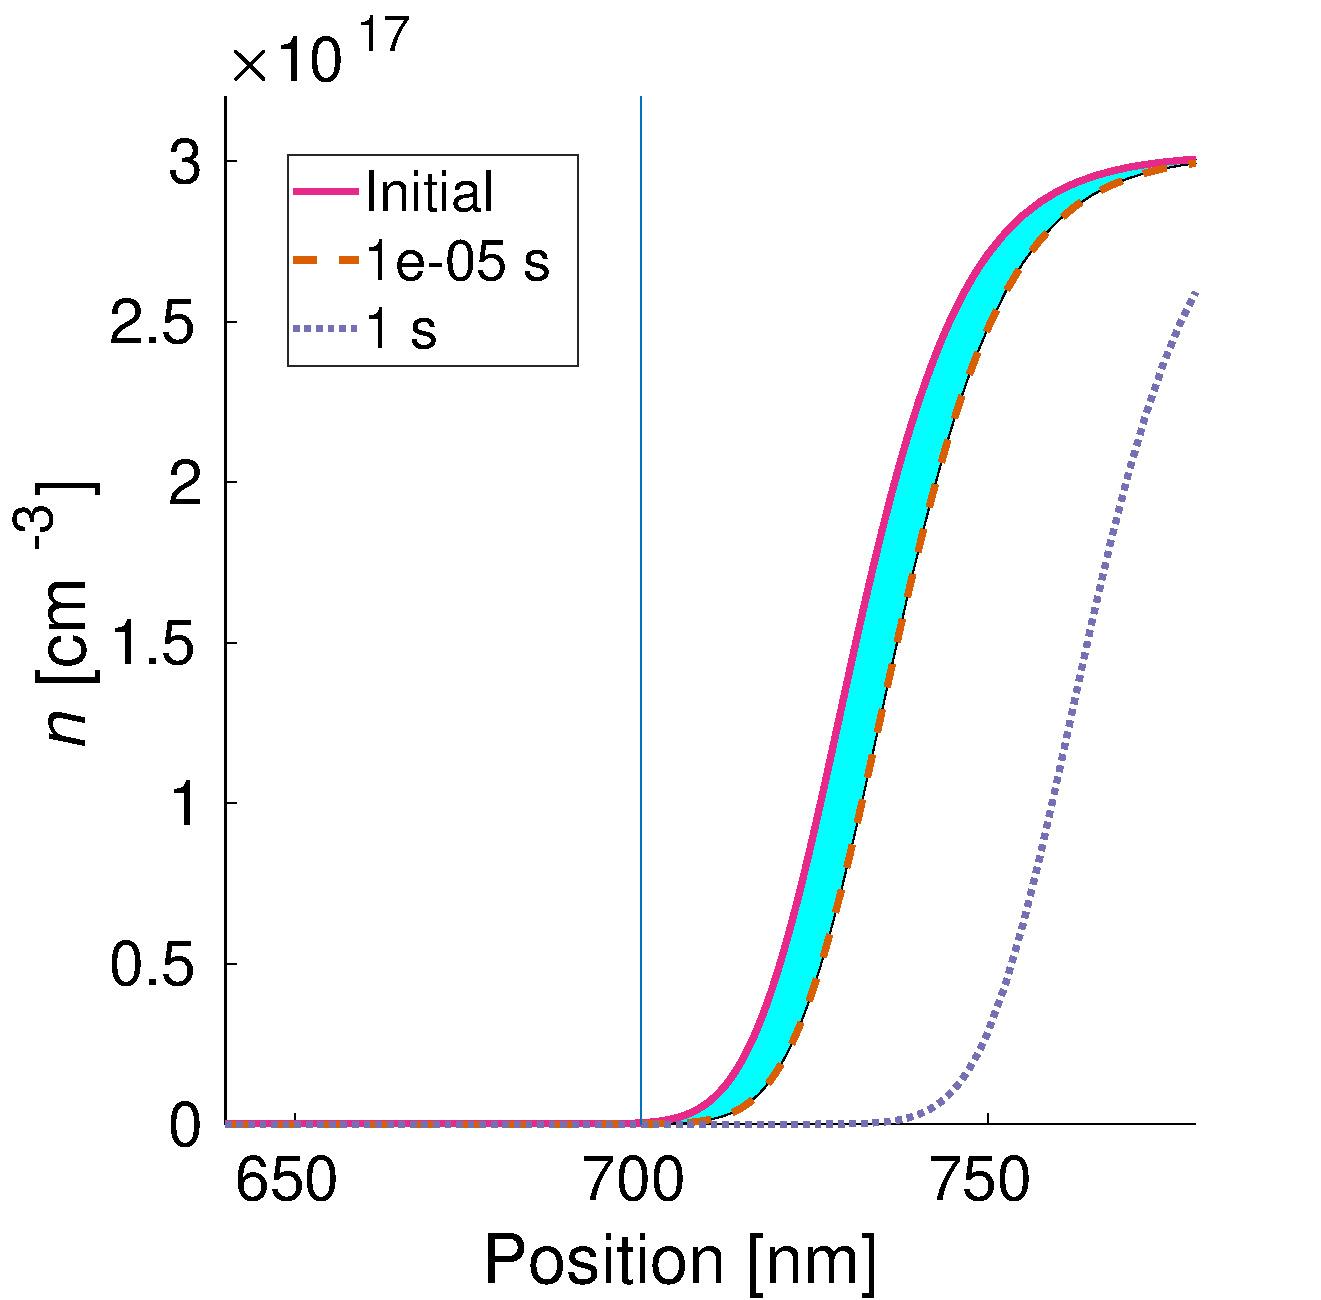
\includegraphics[width=1\textwidth]{ce_single_dd_charge/ce_ions_1sun.pdf}
						\subcaption{1 sun}\label{fig:ce_single_dd_charge-1sun}
					\end{subfigure}
					\qquad
					\begin{subfigure}[t]{0.51\textwidth}
						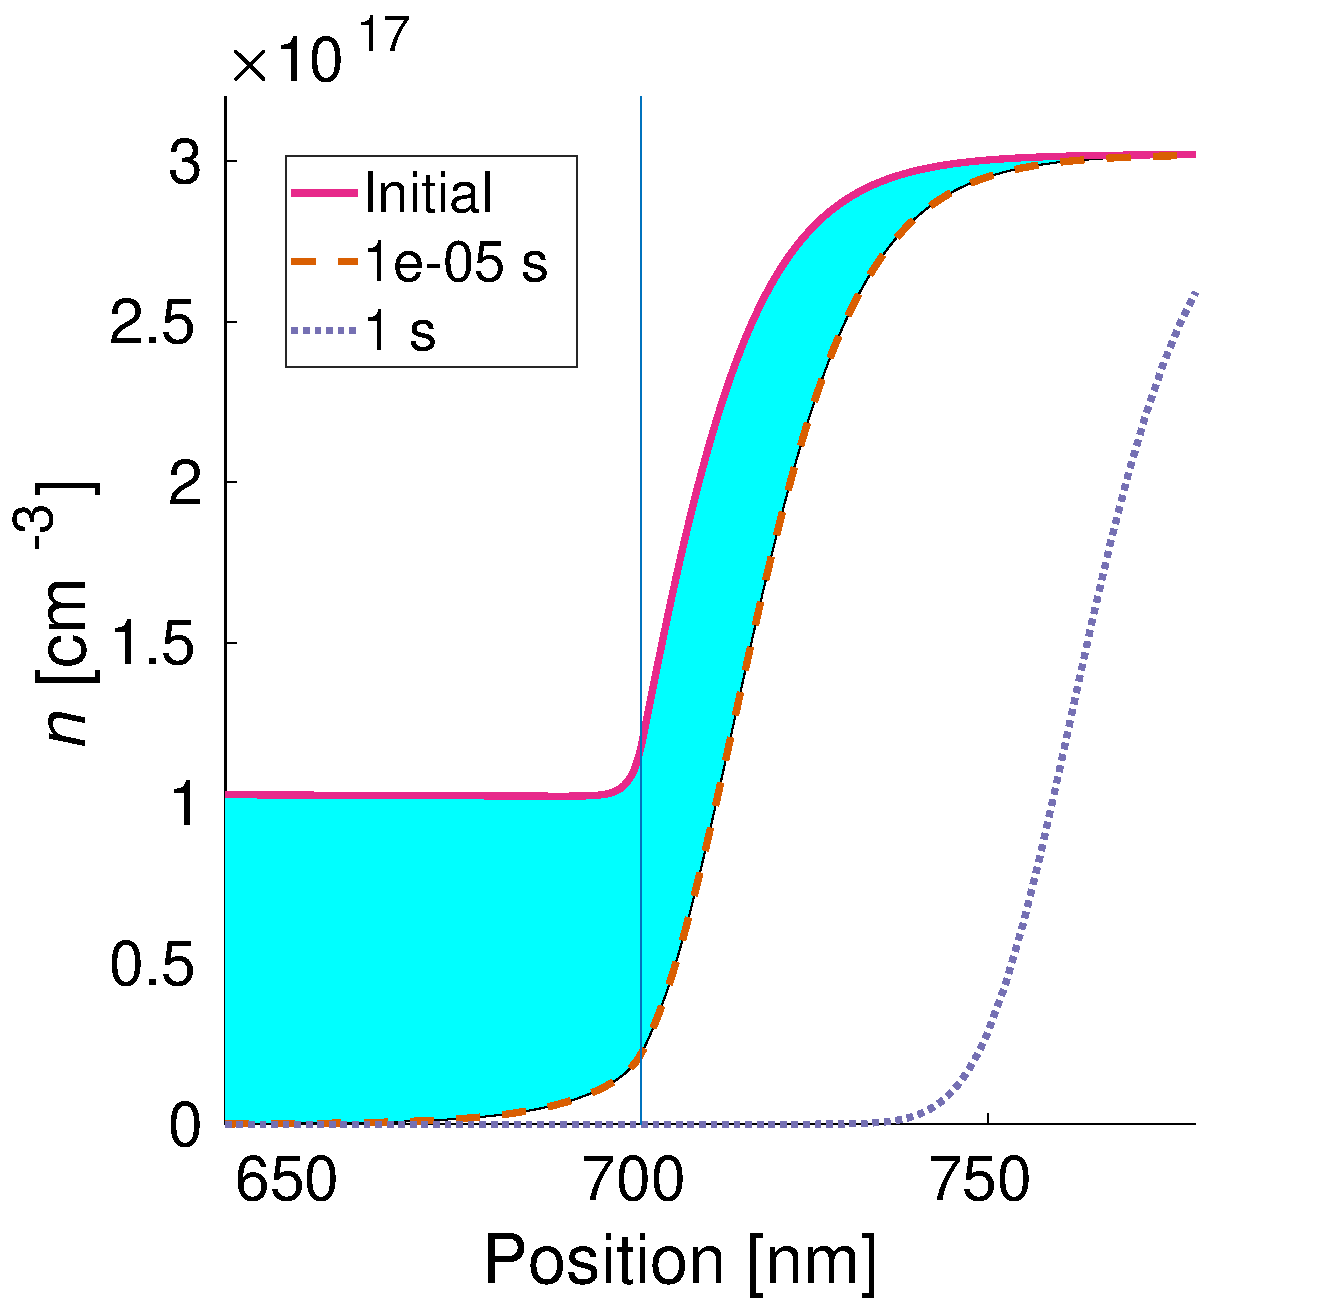
\includegraphics[width=1\textwidth]{ce_single_dd_charge/ce_ions_1000suns.pdf}
						\subcaption{1000 suns}\label{fig:ce_single_dd_charge-1000suns}
					\end{subfigure}

					\mycaption[Simulated electron density profile during a CE experiment.]{
						The electron density profile of a homojunction cell with mobile ions is plotted at the interface between perovskite (position \SI{< 700}{\nm}) and \acr{etm} (position \SI{> 700}{\nm}) at different times during a \acr{ce} experiment.
						The green solid line represent the situation as stabilised at open circuit conditions, before the \acr{ce} experiment. Corresponding energy levels for (\textbf{a}) in \cref{fig:ce_single_dd_levels-1sun} and for (\textbf{b}) in \cref{fig:ce_single_dd_levels-1000suns}.
						The dashed orange line represent the profile at short times, after the extraction of the free charges but before the reorganization of the mobile ions.
						The light blue area represents the extra charge extracted during a typical \acr{ce} experiment.
						In (\textbf{a}) the device is stabilised at 1 sun light intensity before performing the charge extraction, in this case most of the extra charge is accumulated in the contacts.
						In (\textbf{b}) the device is stabilised at 1000 suns, in which case the charge is mainly accumulated in the perovskite layer.
						The dotted violet line is the final electronic profile, at long times after the mobile ions migration, which is identical for (\textbf{a}) and (\textbf{b}) cases. Corresponding energy levels in \cref{fig:ce_single_dd_levels-dark}.
						\Gls{ce} simulation routines explained in \cpageref{dd_ce}.
					}\label{fig:ce_single_dd_charge}
				}
			}
		\end{figure}

		\paragraph{Linear part and geometric capacitance\index{geometric capacitance}}\label{geometric_capacitance}
		With the introduction of selective contacts, a linear contribution starts to grow in importance summing up to the exponential part.
		It has been observed both in \gls{osc} \cite{Ryan2017a,Credgington2014,Credgington2012} and in perovskite solar cells \cite{Gelmetti2017,Wheeler2017,Du2018}.
		This linear trend accounts for the accumulation in the selective contacts' depletion\index{space charge layer} layers and in the electrodes, in a parallel plate capacitor fashion: $n = C_|g| \cdot V = \frac{\epsilon_0 \epsilon_|r| A}{d} \cdot V$ where $C_|g|$ is the geometric capacitance\index{geometric capacitance}, $A$ is the active area, $d$ is the thickness of the dielectric, $\epsilon_0$ is the electric constant, and $\epsilon_|r|$ is the relative permittivity.
		This carriers accumulation in the contacts can be visualized with the simulation reported in \cref{fig:ce_single_dd_charge-1sun}.
		Extending \cref{eq:ce_osc}, the complete equation becomes:
		\begin{equation}\label{eq:ce_full}
			n_|CE|(V) = C_|g| \cdot V + n_|eq| \cdot \left[\exp(\frac{qV}{mk_|B|T}) - 1\right]
		\end{equation}

		\paragraph{Geometric capacitance voltage dependency}\label{geometric_capacitance_and_voltage}
		More exactly, $d$ is the distance between the regions where the opposed charges are getting accumulated, which is the space\index{space charge layer} charge layers (usually depletion\index{space charge layer} layers) in the contacts.
		So this value can be somewhat wider than just the distance separating the two perovskite/contacts interfaces.
		By consequence, $\epsilon_|r|$ should be considered as a thickness\hyp{}weighted mean of the relative permittivities of each material between the two accumulation zones.
		Moreover, as the depletion\index{space charge layer} layers fill up they widen and shrink, so this capacitance can vary as happens for the junction capacitance (\textsl{i.e.}\ transition capacitance) of a $p$-$n$ junction.
		A voltage dependent geometric capacitance\index{geometric capacitance} can be obtained from dark \acr{ce} measurements applying reverse voltage biases \cite{Kiermasch2018} or \textsl{via} impedance spectroscopy in dark with a constant voltage bias \cite{Brus2016,Pockett2015}.
		While this dependency cannot be ignored in silicon solar cells or in \gls{osc}, where the $n$ and the $p$-type materials are in close contact, it is likely negligible in perovskite solar cells as the change of depletion\index{space charge layer} layers thickness (Debye length), happening in the contacts, is negligible when summed to the perovskite layer thickness.

		\paragraph{Energy levels point of view}\label{ce_energy_levels}
		As we mentioned, the linear trend is related to the accumulation in the contacts depletion\index{space charge layer} layers (or, generically, space\index{space charge layer} charge layers), this can be seen from the decrease of the perovskite\hyp{}contacts conduction band offset between \cref{fig:ce_single_dd_levels-dark,,fig:ce_single_dd_levels-1sun}.
		Increasing the light illumination at open circuit conditions, the quasi\hyp{}Fermi levels splitting approaches the built\hyp{}in voltage represented by the contacts' band edges: $qV_|BI| = \bar\mu^{\mathrm{cathode}} - \bar\mu^{\mathrm{anode}} \approx \bar\mu_|CB|^{\mathrm{ETM}} - \bar\mu_|VB|^{\mathrm{HTM}}$.
		This means the depletion\index{space charge layer} layers are close to saturation, like in \cref{fig:ce_single_dd_levels-1000suns} where \SI{1000}{suns} illumination was simulated, and the charge accumulates in the perovskite layer, as shown in \cref{fig:ce_single_dd_charge-1000suns}, and the exponential trend gains importance.

		\begin{figure}
			\makebox[\textwidth][c]{
				\parbox{1.1\textwidth}{
					\centering
					\begin{subfigure}[t]{0.31\textwidth}
						\includegraphics[width=1\textwidth]{ce_single_dd_levels/ce_ions_dark_levels.pdf}
						\subcaption{dark}\label{fig:ce_single_dd_levels-dark}
					\end{subfigure}
					\qquad
					\begin{subfigure}[t]{0.31\textwidth}
						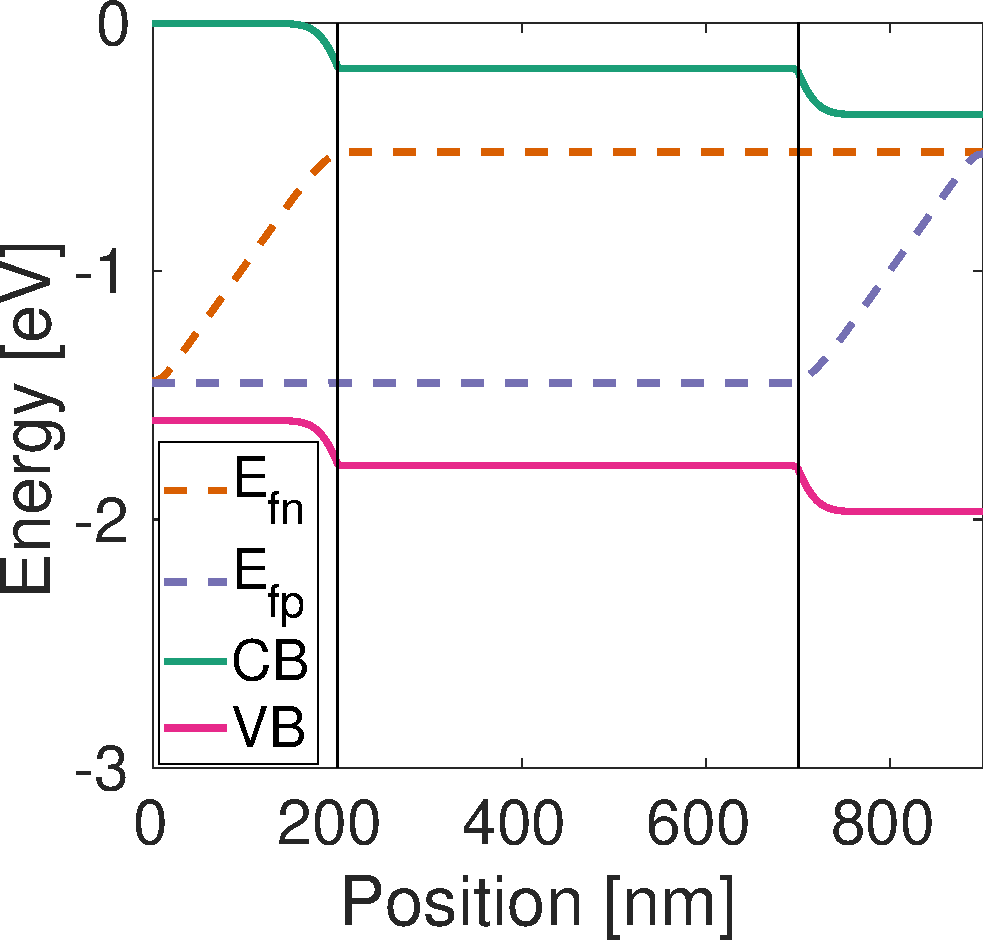
\includegraphics[width=1\textwidth]{ce_single_dd_levels/ce_ions_1sun_levels.pdf}
						\subcaption{1 sun, OC}\label{fig:ce_single_dd_levels-1sun}
					\end{subfigure}
					\qquad
					\begin{subfigure}[t]{0.31\textwidth}
						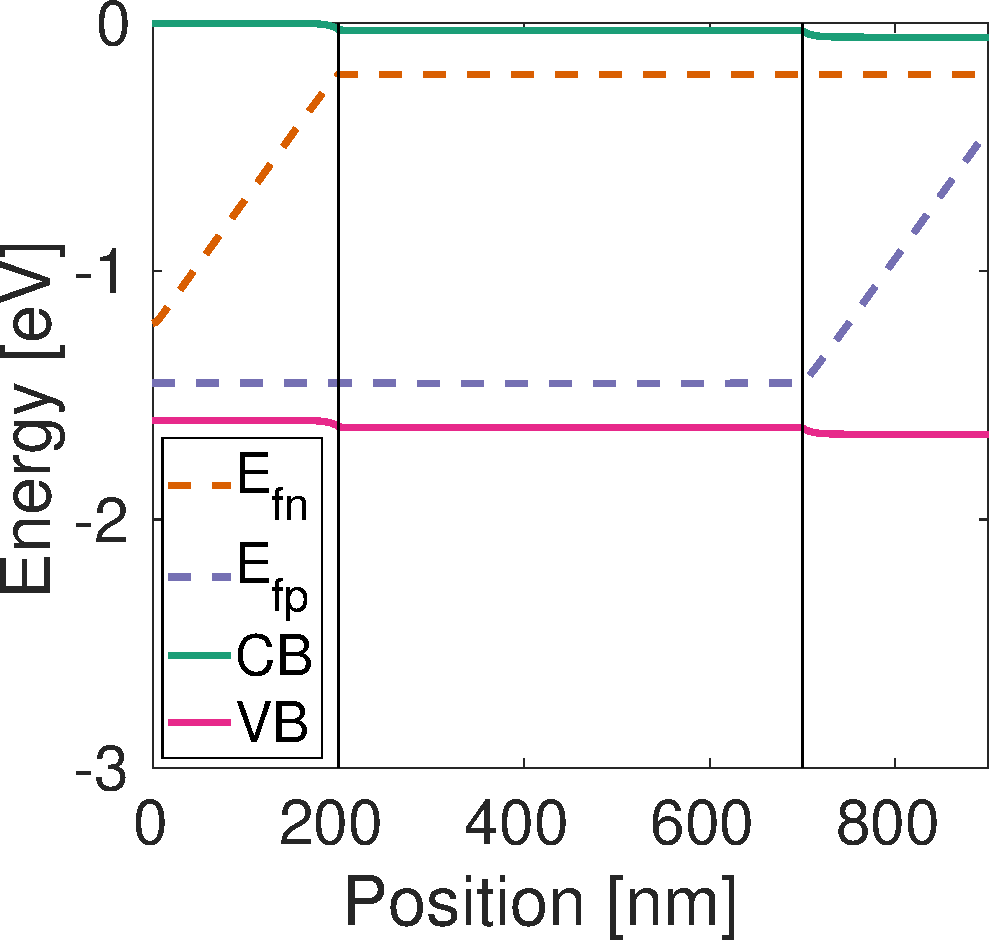
\includegraphics[width=1\textwidth]{ce_single_dd_levels/ce_ions_1000suns_levels.pdf}
						\subcaption{1000 suns, OC}\label{fig:ce_single_dd_levels-1000suns}
					\end{subfigure}

					\mycaption[Simulated energy levels in a homojunction device with mobile ions at open circuit conditions at different light intensities.]{The simulated energy levels of a homojunction $p$(\SI{200}{\nm})--$i$(\SI{500}{\nm})--$n$(\SI{200}{\nm}) device with mobile ions in the intrinsic layer. In (\textbf{a}) the device is in dark, in (\textbf{b}) it is illuminated at \SI{1}{sun} light intensity, and in (\textbf{c}) illuminated at \SI{1000}{suns}.
					}\label{fig:ce_single_dd_levels}
				}
			}
		\end{figure}

	\subsection{Interpretation of CE \textsl{versus} Light Bias With Mobile Ions}

		\paragraph{Linear part with mobile ions}\label{ce_ions_linear}
		The presence of mobile ions in perovskite materials which can accumulate at the perovskite/contacts interfaces, adds an additional capacitance $C_|ion|$, which replaces the geometric capacitance\index{geometric capacitance} $C_|g|$ at low frequencies or long time scales, as we showed in \authoryear{Moia2019}.
		Comparing the initial electrostatic potential profile with the electrostatic potential at long times, after the ionic migration, we can see that there is no electric field in the bulk of the perovskite layer neither at the beginning neither at the end of the measurement.
		This means that the capacitance we can observe at long times or slow frequencies is not the geometric one, but rather the ionic one across each of the interfaces which is expected to be independent on the device's thickness.
		Nevertheless, as pointed out in \cpageref{ce_limitations_perovskite}, the \acr{ce} measurements are never carried on for long enough to include the ionic migration, and so also the ionic accumulation capacitance is not observed in our experiments.
		This can be visualized with the simulation reported in \cref{fig:ce_full_dd} where the long timescale (where the current is monitored until complete stabilisation) and the short timescale (few tens of microseconds) \acr{ce} experiment are compared.
		The difference between the short and long timescale extracted charges is the linear contribution by the ionic capacitance discharge, observable as electronic current thanks to the relative displacement current\index{displacement current}.
		A simulation with frozen ions (the ionic profile was stabilised at open circuit and frozen during the \acr{ce} experiment) was also performed but not reported.
		For this case, the simulated extracted charge was identical to the reported short timescale extraction simulation in \cref{fig:ce_full_dd}.

		\begin{figure}%[!hbtp]%
			\makebox[\textwidth][c]{
				\parbox{1.1\textwidth}{
					\centering
					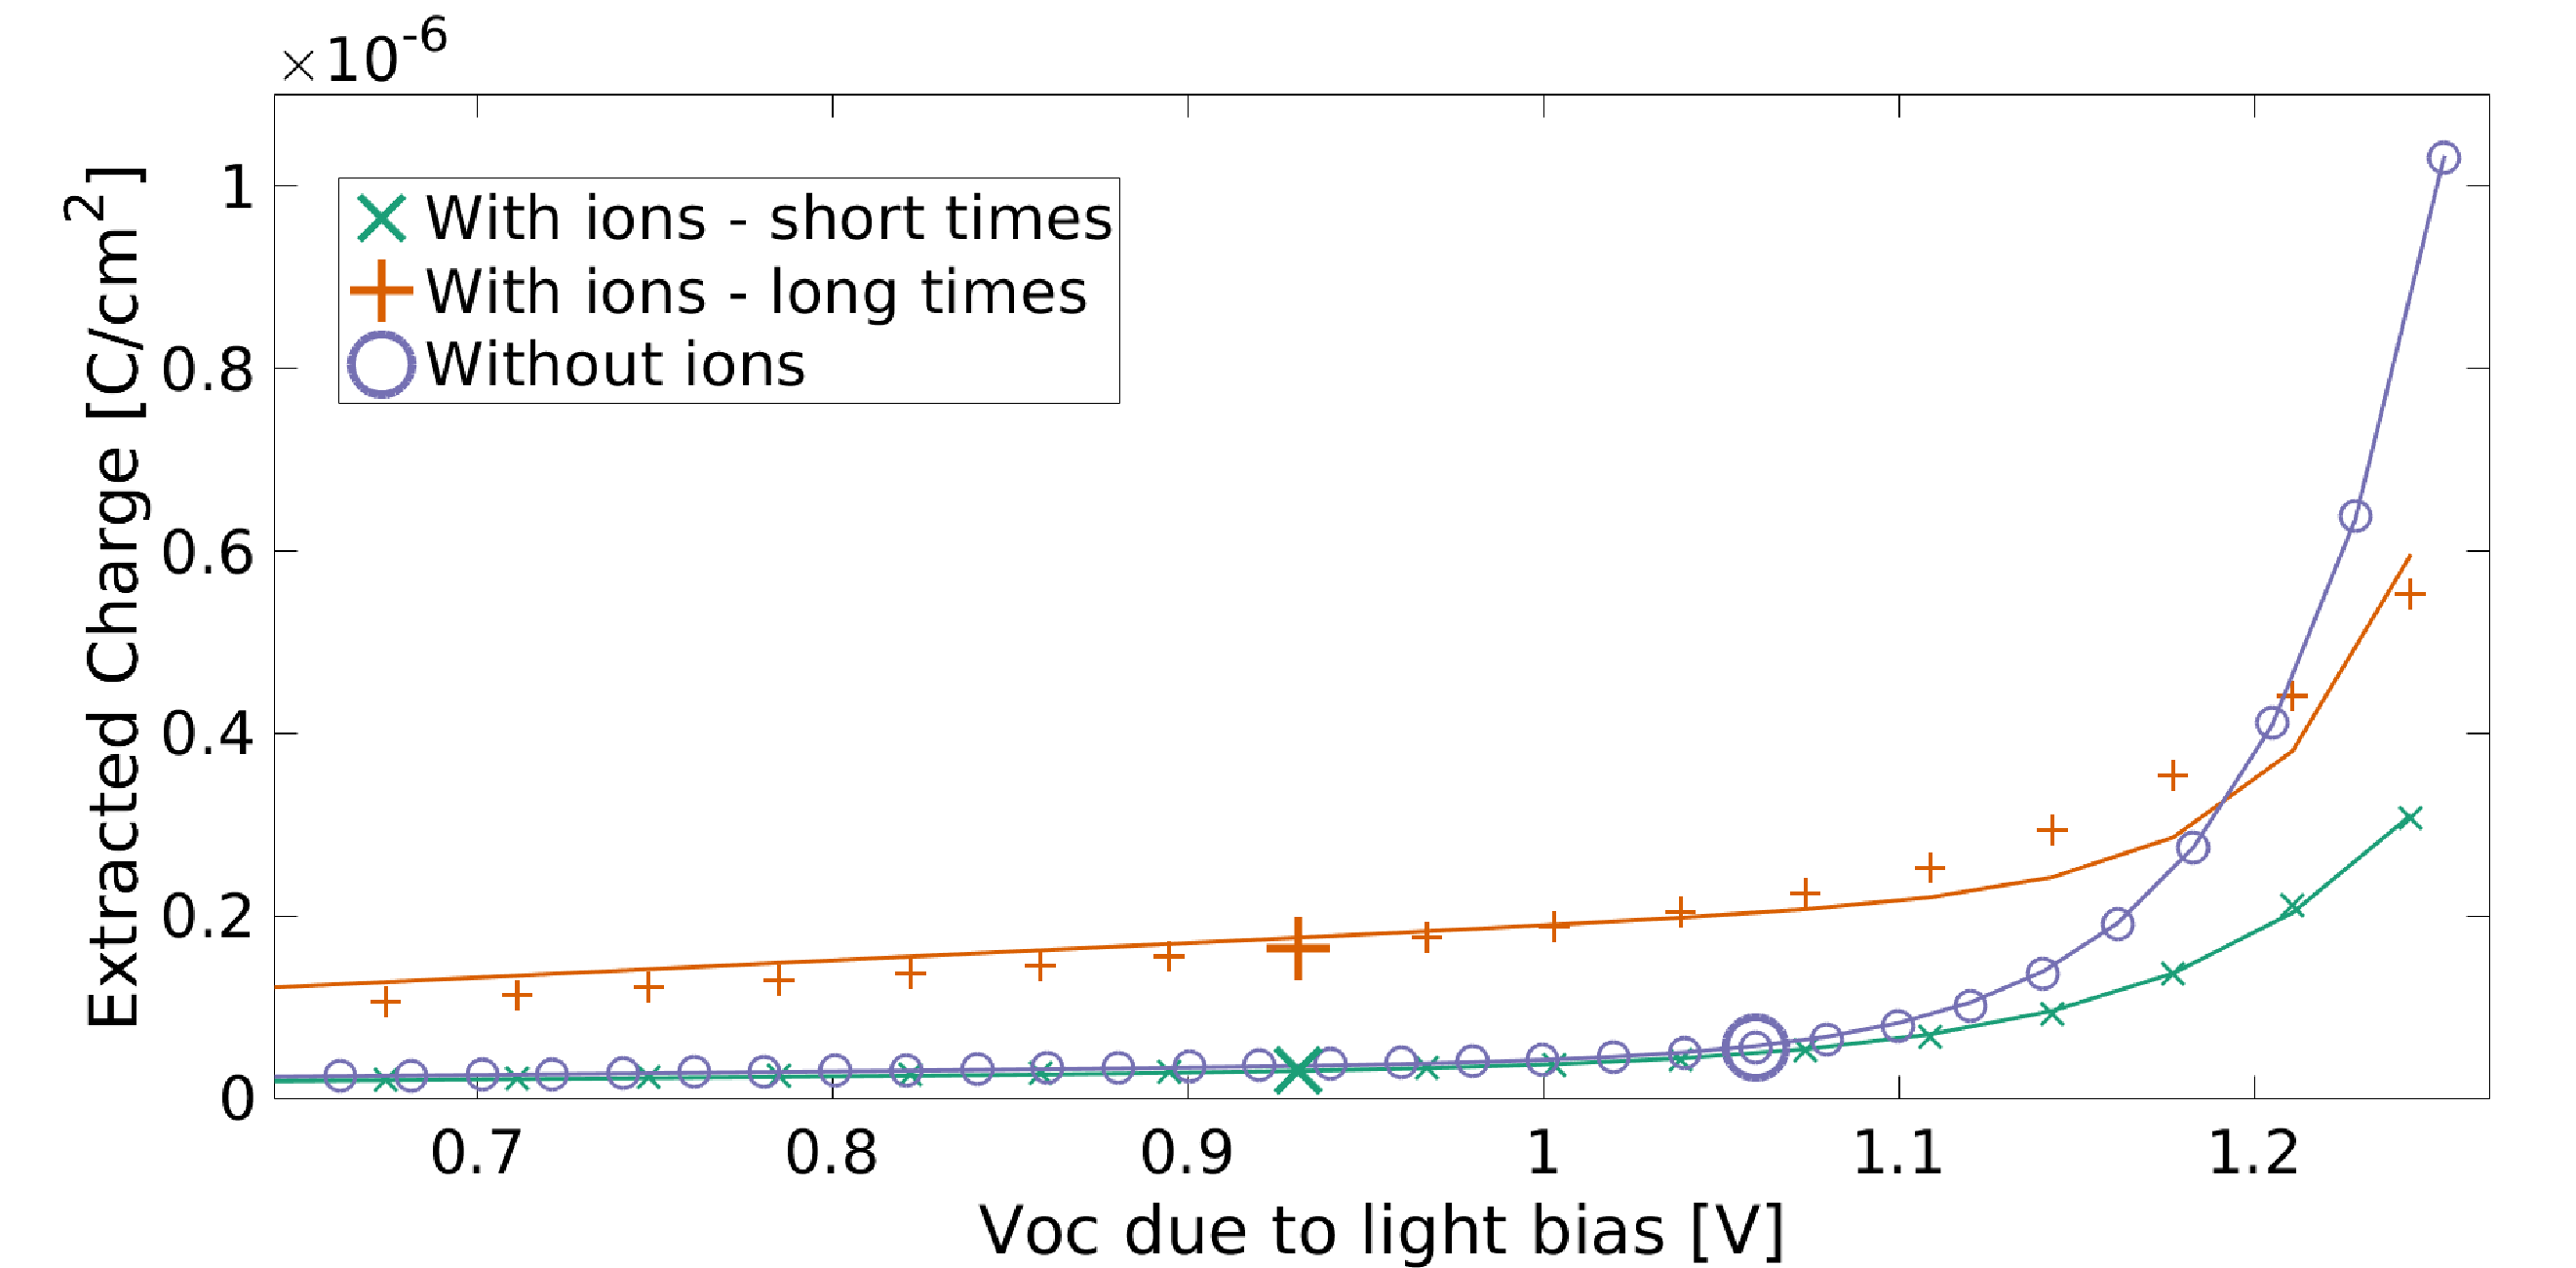
\includegraphics[width=0.9\textwidth]{ce_full_dd/ce_full_dd.pdf}
					\mycaption[Simulation of a complete CE experiment: charge \textsl{versus} light bias with or without mobile ions.]{
						A simulation for a homojunction device up to 1000~sun illumination (rightmost point of each set) is reported, with three points for decade.
						For each set of points, the bigger size one indicates the 1~sun pre\hyp{}illumination.
						The green crosses simulates the experimentally utilised conditions: the charge gets integrated over few microseconds, while the mobile ions did not have enough time to start migrating.
						The orange pluses considers the charge integrated until the device stabilisation, over various seconds, including also the ionic displacement current\index{displacement current}.
						The purple circles simulates a mobile ions free device.
						The solid lines represents the linear plus exponential fit crossing (0,0) obtained with the \cref{eq:ce_full} $n_|CE| = C_|g| V + n_|eq| \{\exp[q V / (mk_|B|T)] - 1\}$ where $C_|g|$, $n_|eq|$, and $m$ are free fitting parameters whose meaning is described in the text.
					\Gls{ce} simulation routines explained in \cpageref{dd_ce}.
				}\label{fig:ce_full_dd}
				}
			}
		\end{figure}

		\paragraph{Exponential part with or without mobile ions}
		As can be seen in \cref{fig:ce_full_dd}, the simulated geometric capacitance\index{geometric capacitance} is similar to the one obtained from short time extraction with mobile ions but the exponential part is considerably different.
		%		when a device with no mobile ions is simulated, longer extraction time doesn't result in more charge, as expected due to the suppression of the ionic contribution.
		This is caused by the very different free charge accumulation profile: the presence of an un\hyp{}shielded electric field in the absorber layer causes the free carriers to accumulate close to the respective selective layer, in other words it keeps the charges away from the respective recombination centres (\textsl{e.g.}\ perovskite/\gls{htm} for electrons).
		This allows the simulated ions free device to store more charge at the same illumination intensity.

		\FloatBarrier
		\newpage
\section{Transient PhotoVoltage (TPV)}\label{characterization_tpv}
	\epigraph{\textit{\enquote{Imma firin mah lazor\\pewpew pewpewpew}}}

	\paragraph{Concept}
	%	While a complete device is kept open circuit under constant illumination, a small extra illumination is added \textsl{via} a short laser pulse.
	This technique allows us to induce a perturbation to a solar cell at open circuit under illumination and observe how it behaves.
	The device at steady state is perturbed photo\hyp{}generating an additional small amount of charge, then we observe the perturbed open circuit voltage dynamics.
	As represented in \cref{fig:tpv_scheme}, the \gls{voc} originally at its steady state value, will increase due to the greater generation rate during the laser pulse.
	%	From the \gls{voc} \textsl{versus} illumination relation for photodiodes reported in \cref{eq:voc_vs_phi} follows that the \gls{voc}, at this new higher illumination, increases (this is not always the case, as for non-stabilised perovskite solar cells \cite{Calado2016}).
	After the end of the short pulse, the \gls{voc} will slowly go back to the steady state value relative to the constant illumination.
	The dynamics of this \gls{voc} relaxation back to the steady state value is the focus of Transient PhotoVoltage experiments (also known as PhotoVoltage Decay experiments) which has been applied to \gls{osc} \cite{Shuttle2008}, to \gls{dssc} \cite{ORegan2005,ORegan2004,ORegan2006}, and recently also to perovskite solar cells \cite{Roiati2014a,Marin-Beloqui2014}.
	From this kinetic profile, a charge lifetime can be obtained and plotted against the light bias due to the constant background illumination, as in the example of \cref{fig:tpv-monoexp}.
	This gives us information about the dominant recombination rate and its dependence on the light bias.

	\begin{SCfigure}
		\centering
		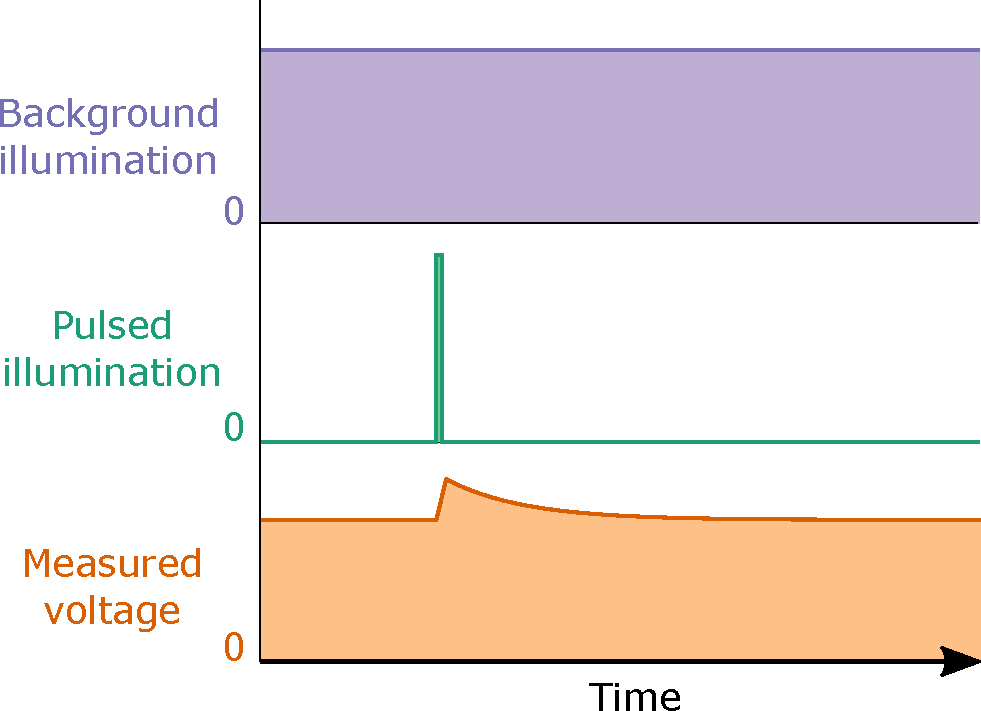
\includegraphics[width=0.65\textwidth]{tpv_scheme/tpv_scheme.pdf}
		\mycaption[Scheme of TPV experiment.]{
			A pulsed illumination sums on the constant background illumination, the measured open circuit voltage dynamic shows an increase and a relaxation. }\label{fig:tpv_scheme}
	\end{SCfigure}

	\paragraph{Procedure}
	The device is kept under constant illumination by a white \gls{led} ring at open circuit until stabilisation is reached.
	Failure to reach stabilisation of the ionic profile will affect the measurement results \cite{ORegan2015b} and can cause unexpected negative \acr{tpv} peaks \cite{Calado2016}.
	Then an additional short illumination pulse is provided using a nitrogen laser.
	The pulse duration (\SI{\approx 1.5}{\ns}) is shorter than the oscilloscope resolution we usually employ, so we assume that the measurement happens when the pulse is already over.
	In the literature, this is not always the case as other research groups use a \gls{led} diode for the pulsed illumination \cite{Calado2016}.
	Usually a wavelength of \SI{590}{\nm} is selected using a Rhodamine 6G solution \cite{RadiantDyesLaser}, this wavelength illuminates in depth the perovskite layer (in contrast to a blue light where the illumination would be absorbed within the first hundreds of nanometres of the material \cite{Bi2016,Tress2016}).
	During all the process, the device is connected to an oscilloscope, registering the open circuit voltage profile (the \SI{1}{\Mohm} resistance of the oscilloscope is a good approximation of open circuit).
	The voltage profile gets averaged over a few tens of pulses in order to increase the signal to noise ratio.
	Initially the light illumination is set to \SI{1}{sun} and the laser pulse intensity is attenuated using a neutral filter so that the voltage perturbation remains smaller than \SI{10}{\mV} for ensuring the small perturbation regime.
	The measurement is repeated after decreasing the background light intensity and waiting a stabilisation time.
	The fitted small perturbation lifetime is plotted \textsl{versus} the light bias.
	The background illumination is decreased down to dark background illumination over a few tens different intensities.
	1~sun equivalent illumination is defined as the illumination at which a silicon photodiode gives the same \gls{jsc} as under calibrated 1~sun from the solar simulator.

	\paragraph{Noise treatment}\label{tpv_robust}
	Most of the observed noise (\SI{< 2E-7}{\s}) is due to the radiofrequency emitted by the spark in the nitrogen laser which gets received by all the non\hyp{}coaxial cables (coaxial ones do not) and from the circuitry of the samples holder acting as an antenna.
	On the contrary to what happens for \acr{ce} (see \cpageref{ce_noise}), the short times noise does not follow a constant pattern, so averaging the measurement over a few repetitions (usually 30) manages to reduce the noise.
	This noise can affect the exponential or bi\hyp{}exponential fitting, for this reason a robust fitting routine has been used, which gives a lower weight to outlier points.
	An example can be seen in \cref{fig:tpv_robust}.

	\begin{figure}
		\makebox[\textwidth][c]{
			\parbox{1.1\textwidth}{
				\centering
				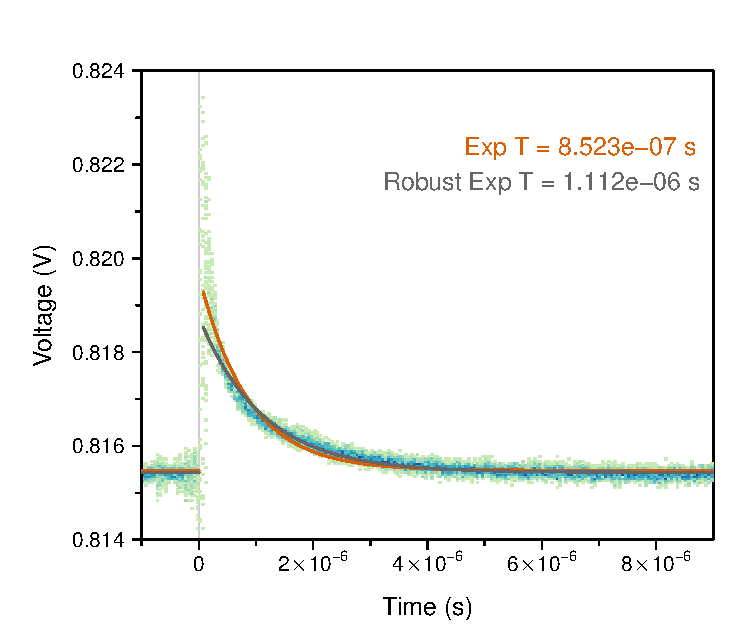
\includegraphics[width=0.8\textwidth]{{tpv_robust/TPV_ig101-1555-1_0.815394_V-monoexp}.pdf}
				\mycaption[Robust and normal fitting comparison.]{Plot of a voltage profile from a single \acr{tpv} decay.
					The 12500 voltage points are represented in a 2D histogram for avoiding the overplotting problem.
					The normal non\hyp{}linear least squares fitting (in orange) is affected by initial noise (a faster decay if we consider this as a bi\hyp{}exponential decay), outliers and characteristics not of interest by the model.
					The non\hyp{}linear robust fitting (in magenta) manages to reduce the weight of these points.
					The studied device is a \gls{fto}\-/\ch{d-TiO2}\-/\gls{csfamapbibr}\-/\gls{tae4}\-/\ch{Au} \cite{Gelmetti2019} with 1~sun background illumination.}\label{fig:tpv_robust}
			}}
	\end{figure}

	\paragraph{Importance of stable steady state starting point}\label{tpv_negativePeaks}
	The values extracted from \acr{tpv} are strongly sensible to the surface recombination and electric fields in the absorber, which in turn vary during ionic profile stabilisation.
	Comparison of decay times with different stabilisation times can be found in \authoryear{ORegan2015b}, while in \authoryear{Calado2016} even negative peaks are reported and explained with the presence of a residual electric field in the absorber previous to ionic profile stabilisation.

	\paragraph{Small perturbations regime}\label{tpv_perturbation}
	The intensity of the laser pulse is attenuated using a variable neutral density filter (a partially reflecting wheel with different positions for different transmittivities) so that the voltage perturbation caused by the light pulse does not exceed \SI{10}{\mV} with 1~sun background illumination intensity.
	We consider this a "small\hyp{}enough" perturbation with regards to the measured \gls{voc} (see \cpageref{perturbation} for a definition of small perturbation).
	For example, comparing the excess charge in a \gls{fto}\-/\ch{d-TiO2}\-/\gls{csfamapbibr}\-/\gls{spiro}\-/\ch{Au} solar cell at \gls{voc} and at \gls{voc}~+~\SI{10}{\mV} which can be obtained from the data in \cref{fig:ce_noise-integrateExp} fitted with \cref{eq:ce_full} we can obtain respectively a value of \SI{8.2E-8}{} and \SI{8.9E-8}{\coulomb\per\square\cm}.
	%Even if we're not considering the dark charge concentration (not measurable in a \acr{ce} experiment), the smallness of the charge perturbation is arguable.
	A smaller perturbation is not practically doable as we are limited to \SI{> 3}{\mV} perturbations due to the strong noise observed in this transient measurement.
	%Clearly, the pulse intensity which could be considered a "small-enough" perturbation at high background illumination is not small any more at lower illumination and definitively cannot be small at dark background conditions.
	Decreasing the background light bias, the laser light pulse intensity is kept constant even when it gets out from small perturbation regime, this is needed in order to be able to use the \acr{tpv} data for calculating \acr{dc}, as explained in \cpageref{dc_perturbation}.
	%We could regulate the pulse intensity depending on the background light intensity, to ensure its smallness, but we \emph{do not} do this in order 
	This does not affect the parameter extraction from \acr{tpv} as just the high illumination intensity points are considered, as seen in \cpageref{tpv_tau_vs_intensity}, in order to study the device close to its expected working conditions.

	\subsection{Interpretation of TPV Mono\hyp{}Exponential Decays}

		\paragraph{Voltage transient and charge concentration relationship}
		As we assume to be in the small perturbation regime, we can study the \cref{eq:ce_full} up to the first term of its series expansion:
		\begin{dmath}\label{eq:tpv_n_deltaV}
			n(V_0 + \Delta V) \approx n(V_0) + \Delta V \cdot \left.\frac{\partial n}{\partial V}\right\rvert_{V=V_0} = n(V_0) + \Delta V \cdot \left[C_|g| + \frac{n_|eq| q}{mk_|B|T}\exp(\frac{qV_0}{mk_|B|T})\right]
			%		n(V_0 + \Delta V) \approx n(V_0) + \Delta V \cdot \eval{\dv{n}{V}}_{V=V_0} = n(V_0) + \Delta V \cdot \left(C_|g| + \frac{n_|eq| q}{mk_|B|T}\exp\left(\frac{qV_0}{mk_|B|T}\right)\right)
		\end{dmath}
		Assigning the last addend to $\Delta n$ we can see that the charge amount variation not only is linear with $\Delta V$ (as we are in the small perturbation regime), but it also depends on the steady state voltage $V_0$.
		This relation is studied in the differential capacitance (\acr{dc}) experiment, described further in this chapter.

		\paragraph{Voltage re\hyp{}equilibration dynamics}
		For what concerns a \acr{tpv} experiment, we are just interested in the analysis of the time needed for re\hyp{}equilibration to steady state conditions.
		As seen in \cref{eq:tpv_n_deltaV}, the relation between $\Delta V$ and $\Delta n$ in small perturbation regime is linear, so the lifetime extracted from a $\Delta V$ decay will have the same lifetime of the underlying $\Delta n$, which is the interesting quantity when speaking of recombination.
		This means that we can observe the variations in voltage for having a correct kinetic description of the charge amount variation.
		At steady state conditions, the time derivative of the amount of charge is zero $\partial n_0 / \partial t = g(\phi) - U(n_0) = 0$ where $g$ is the generation rate and $U$ is the recombination rate.
		Considering the situation after the end of the light pulse, so while $g$ is constant but $n$ has been increased by $\Delta n$, and using a simplified expression for the recombination including just two contributions with reaction order 1 and 2 and rate constants $k_1$ and $k_2$ we can write:
		\begin{dmath}
			%		\frac{\partial (n_0 + \Delta n)}{\partial t} = g - k_1(n_0 + \Delta n) - k_2(n_0 + \Delta n)^2 = (g - k_1 n_0 - k_2 n_0^2) - (k_1 \Delta n + 2 k_2 n_0 \Delta n) - (k_2 \Delta n ^2) \approx - (k_1 + 2 k_2 n_0 ) \Delta n
			\pdv{(n_0 + \Delta n)}{t} = g - U = g - k_1(n_0 + \Delta n) - k_2(n_0 + \Delta n)^2 = (g - k_1 n_0 - k_2 n_0^2) - (k_1 \Delta n + 2 k_2 n_0 \Delta n) - (k_2 \Delta n ^2) \approx - (k_1 + 2 k_2 n_0 ) \Delta n
		\end{dmath}
		where the zeroth order term is the steady state value, so it is zero, and the second order order term can be neglected (if $\Delta n \ll n_0$ then $k_2 \Delta n^2 \ll k_2 n_0 \Delta n$).
		So the rate equation is a simple pseudo first order reaction, and the kinetic behaviour follows an exponential description like:
		\begin{equation}\label{eq:tpv_monoexp}
			n (t) = n_0 + \Delta n_0 \cdot e^{-(k_1 + 2 k_2 n_0) t} = n_0 + \Delta n_0 \cdot e^{-t / \tau}
		\end{equation}
		where $\tau = (k_1 + 2 k_2 n_0)^{-1}$ is the small perturbation lifetime.
		For a single recombination with a generic recombination reaction order $\Phi$ we can generalize to \cite{Shuttle2008}:
		\begin{equation}\label{eq:tpv_tau_order}
			\tau \approx (\Phi k n_0^{\Phi-1})^{-1}
		\end{equation}
		where $k$ is the dominant recombination rate constant.

		\begin{figure}
			\makebox[\textwidth][c]{
				\parbox{1.1\textwidth}{
					\centering
					\begin{subfigure}[t]{0.5\textwidth}
						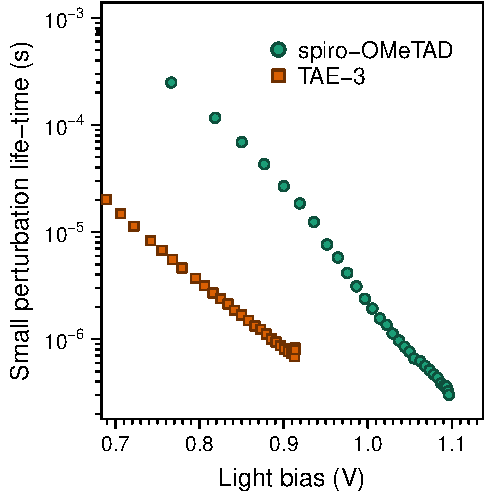
\includegraphics[width=1\textwidth]{tpv/monoexp/spiro_vs_TAEs-TPVs-robustmonoexp-crop.pdf}
						\subcaption{Mono\hyp{}exponential lifetimes \textsl{versus} light bias}\label{fig:tpv-monoexp}
					\end{subfigure}
					\qquad
					\begin{subfigure}[t]{0.5\textwidth}
						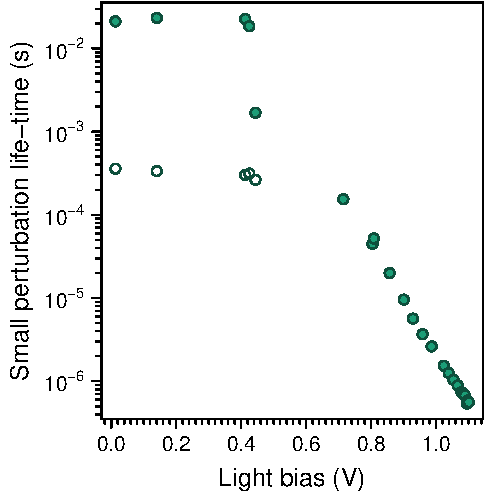
\includegraphics[width=1\textwidth]{tpv/biexp/tpv-tpv-mixedbimono-crop.pdf}
						\subcaption{Bi\hyp{}exponential lifetimes \textsl{versus} light bias for a \gls{famapbibr} device}\label{fig:tpv-biexp_full}
					\end{subfigure}
					\bigskip

					\begin{subfigure}[t]{0.9\textwidth}
						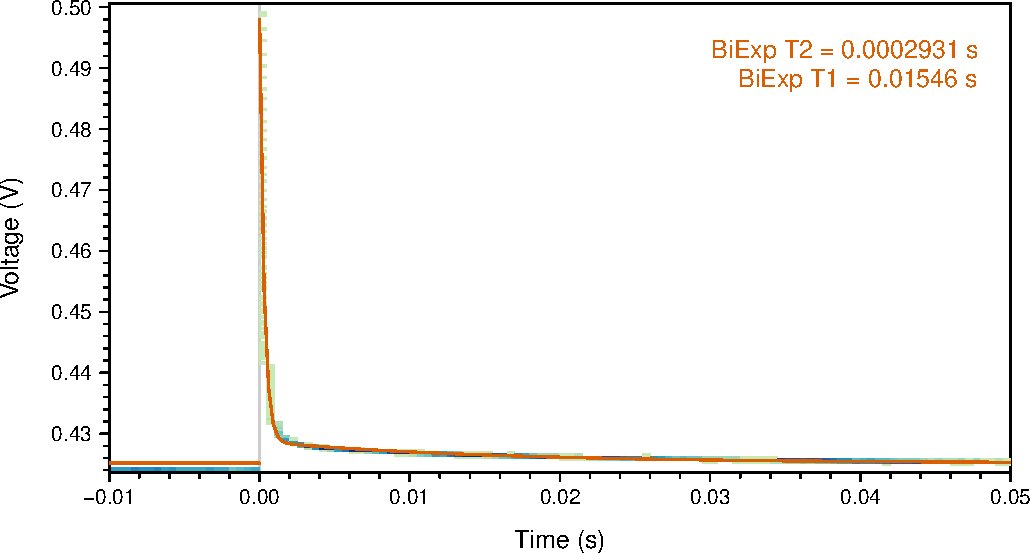
\includegraphics[width=1\textwidth]{{tpv/biexp/tpv/TPV_ig57-475-2_0.424021_V-biexp-crop}.pdf}
						\subcaption{Single bi\hyp{}exponential decay}\label{fig:tpv-biexp_single}
					\end{subfigure}

					\mycaption[Example of lifetimes \textsl{versus} light bias plot obtained from a TPV experiment.]{In (\textbf{a}) the small perturbation lifetimes obtained from robust mono\hyp{}exponential fitting are plotted against light bias for \gls{fto}\-/\ch{d-TiO2}\-/\gls{csfamapbibr}\-/\gls{htm}\-/\ch{Au} devices \cite{Gelmetti2019}. In (\textbf{b}) the lifetimes of a \gls{fto}\-/\ch{d-TiO2}\-/\gls{famapbibr}\-/\gls{spiro}\-/\ch{Au} device as obtained from a robust bi\hyp{}exponential fitting for low light bias, where the decays are clearly biphasic, and mono\hyp{}exponential for higher illuminations. In (\textbf{c}) the full data for the point at \SI{0.42}{V} from (\textbf{b}) is reported.}\label{fig:tpv}
				}
			}
		\end{figure}

	\subsection{Interpretation of TPV Bi\hyp{}Exponential Decays}

		\paragraph{At high background illumination}
		In our simulation, at high illumination intensity we observe just mono\hyp{}exponential voltage decays both without (\cref{fig:tpv_full_dd_noions}) or with mobile ions (\cref{fig:tpv_full_dd_ions}).
		Experimentally, for some devices rather than an exponential decay, a bi\hyp{}exponential voltage decay is observed, like the one reported in \cref{fig:tpv-biexp_single}.
		This is more frequent in bottom cathode devices including mesoporous titania layers \cite{Carnie2015,ORegan2015b,Bertoluzzi2015} but has also been reported for silicon solar cells \cite{Kiermasch2018}.
		With \emph{bi\hyp{}exponential} decay we refer to the sum of two exponential decays with two different half\hyp{}life times, like:
		\begin{equation}\label{eq:tpv_biexp}
			V (t) = V_0 + \Delta V_a \cdot e^{-t/\tau_a} + \Delta V_b \cdot e^{-t/\tau_b}
		\end{equation}
		where $\tau_a$ and $\tau_b$ are two distinct lifetimes while $\Delta V_a$ and $\Delta V_b$ are the respective amplitudes of the contributions to the measured decay.
		The presence of two different recombination processes is not enough for justifying a bi\hyp{}exponential decay.
		This is clear looking to \cref{eq:tpv_monoexp}, where considering two recombination processes with two different reaction orders we obtained a simple exponential decay.
		What we have to remember here, is that \cref{eq:tpv_monoexp} was obtained for a zero dimensional case, like what would happen in a homogeneous chemical reaction.
		In our case, the multiple recombination centres could be spatially separated.
		If the charge concentration in the two centres is dis\hyp{}entangled (is not identical at any time), the sum of two exponential decays can be expected rather than a simple exponential.
		This dis\hyp{}entanglement is possible if the time needed for the free carriers to migrate from a recombination centre to the other is larger than the shorter recombination lifetime.
		This can happen thanks to a large\hyp{}enough distance between recombination centres together with a slow free carriers mobility \cite{Calado2018}.
		For example for recombination centres at different depths in the solar cell stack, like at the two perovskite/contacts interfaces.
		The fact that the presence of mesoporous structures are often present when bi\hyp{}exponential decays are observed can be understood by the smaller mobility of perovskite when intercalated in such structures \cite{Leijtens2014}.
		This have been reported also for laterally distanced recombination centres (\textsl{e.g.}\ pinholes \textsl{versus} well covered regions) by \authoryear{Montcada2017}.
		%	the high mobility in the electrodes is expected to equal the quasi-Fermi levels in the two adjacent recombination centres avoiding bi\hyp{}exponential decays, nevertheless reports of this phenomena have been reported \cite{Montcada2017}.

		\paragraph{Mobility limited case}\label{tpv_mobility}
		As we just saw, the mobility is a crucial parameter for the \acr{tpv} experiment.
		As a mental exercise we can imagine a case where the mobility is so slow that the free charges take a long time to diffuse (we consider diffusion as perovskite solar cells are assumed to be field\hyp{}free in the absorber layer, but the same concept would hold with charges' drift) from the generation zone (in the absorber) to the recombination centre (\textsl{e.g.}\ at a contact/absorber interface).
		In such an extreme case the provisioning of charges to the recombination centres could become a bottleneck rather than the recombination itself.
		A drift\hyp{}diffusion simulation of this can be found in \authoryear{Calado2018}.
		In this regime, a \acr{tpv} experiment would be rather insensitive to actual recombination constants and even to light intensity, giving just information about mobility.
		As the observed \acr{tpv} lifetimes are strongly light\hyp{}intensity dependent, at least at high background illumination, we can exclude to be in this mobility\hyp{}limited regime.
		This would have to be revised in case a strong illumination\hyp{}dependent mobility in perovskite materials was demonstrated, as has been reported in \gls{osc} \cite{Eng2010,Shuttle2010,Deledalle2014}.
		Also a slow trapping and de\hyp{}trapping of the carriers can result in a reduced and illumination\hyp{}dependent mobility \cite{Du2018}.

		\paragraph{Inhomogeneous charge concentration profiles}
		Due to the internal electric field, the free carriers concentration can be inhomogeneous.
		For the surface recombination, this implies that the average excess carriers concentration obtained from \acr{ce} is not necessarily the carriers concentration at the recombination centre \cite{Kirchartz2012}.
		For the band\hyp{}to\hyp{}band recombination, this implies that the $n \cdot p$ product, integrated over the device thickness, can be much smaller than an homogeneous carriers concentration \cite{Deibel2009}.
		These considerations are key for drift\hyp{}driven \gls{osc} with low doping level materials \cite{Deledalle2015,Deledalle2014} but should be of smaller impact for the diffusion\hyp{}driven, field free perovskite solar cells, at least at steady state when the internal electric field is mostly shielded by the ionic accumulation at the interfaces.

	\begin{figure}
	\makebox[\textwidth][c]{
		\parbox{1.1\textwidth}{
			\centering
			\begin{subfigure}[t]{0.51\textwidth}
				\centering
				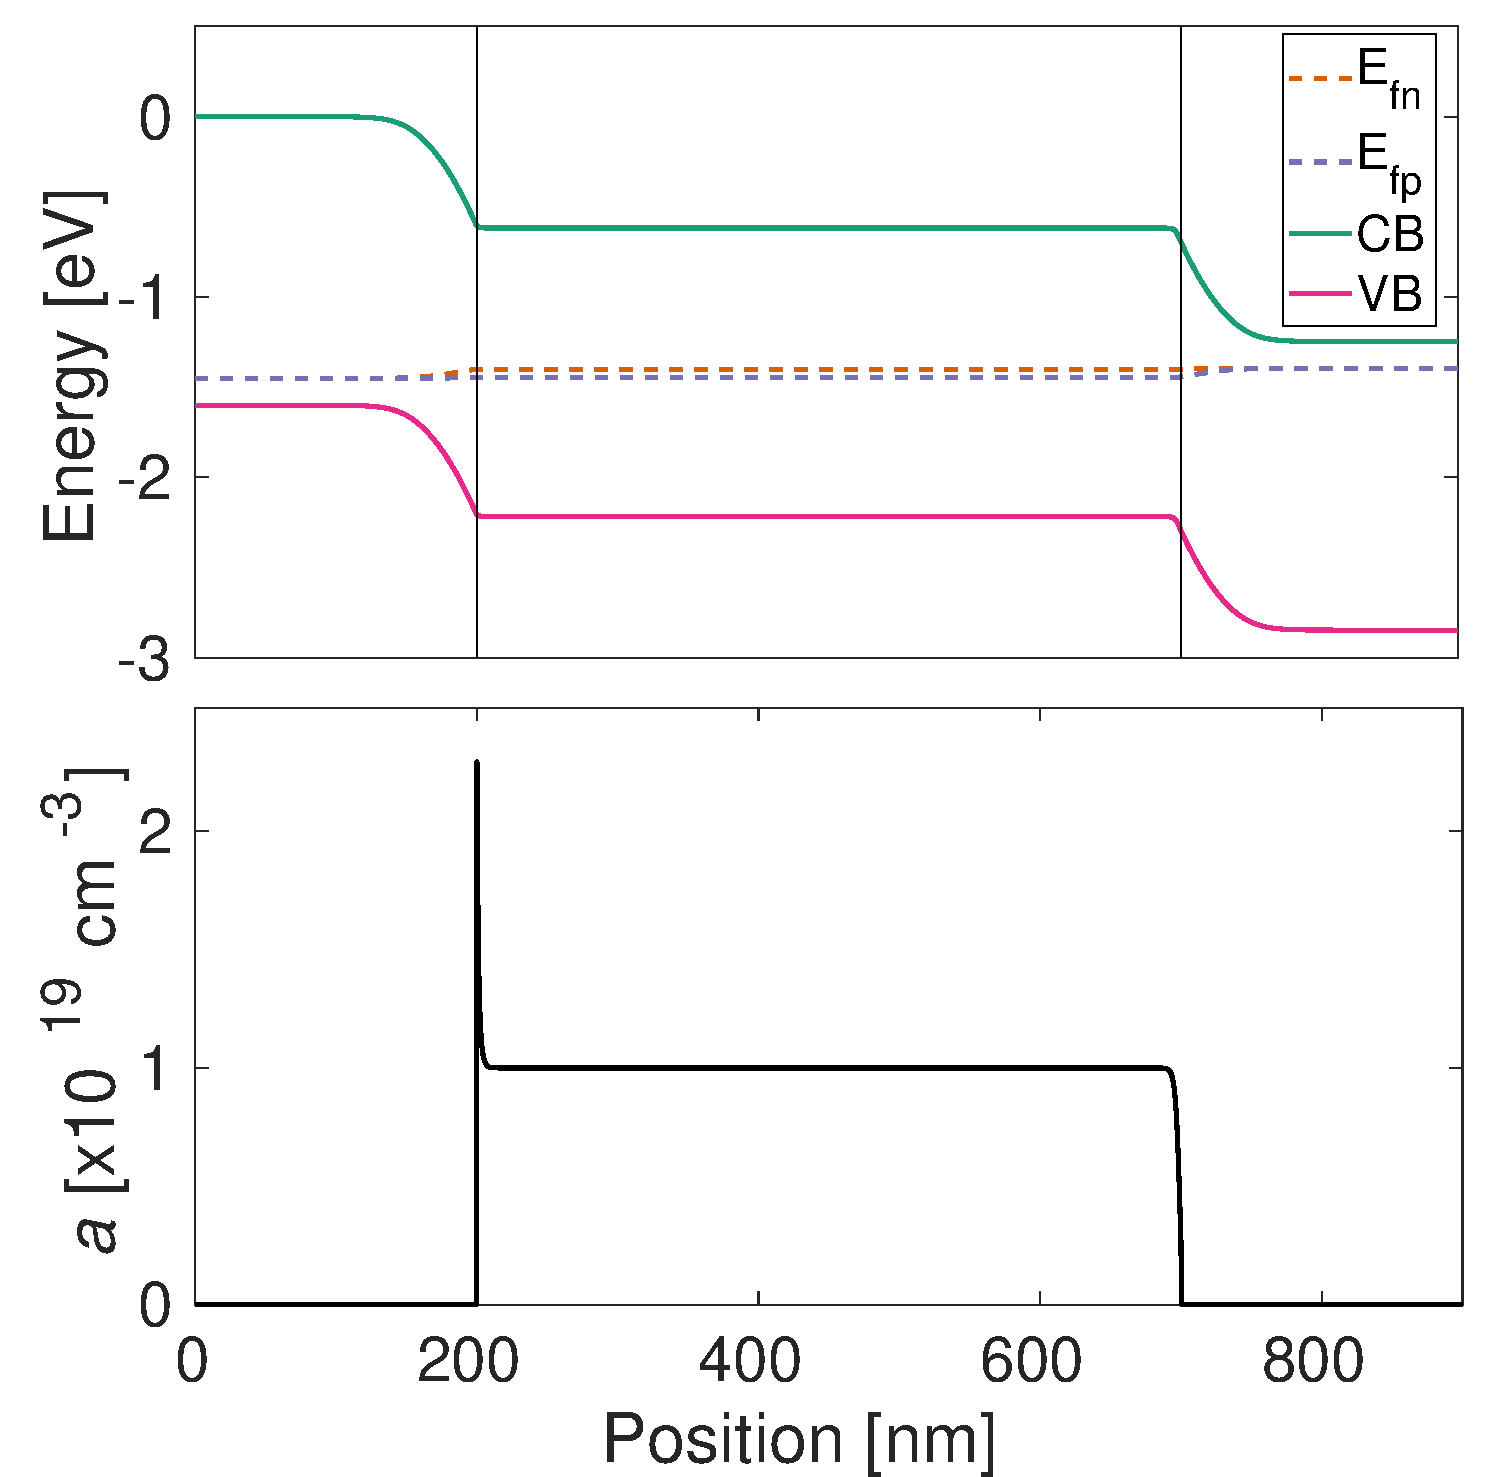
\includegraphics[width=0.9\textwidth]{tpv_ionic/tpv_ionic_reference.pdf}
				\subcaption{Low illumination, steady state.}\label{fig:tpv_ionic-reference}
			\end{subfigure}
			\qquad
			\begin{subfigure}[t]{0.51\textwidth}
				\centering
				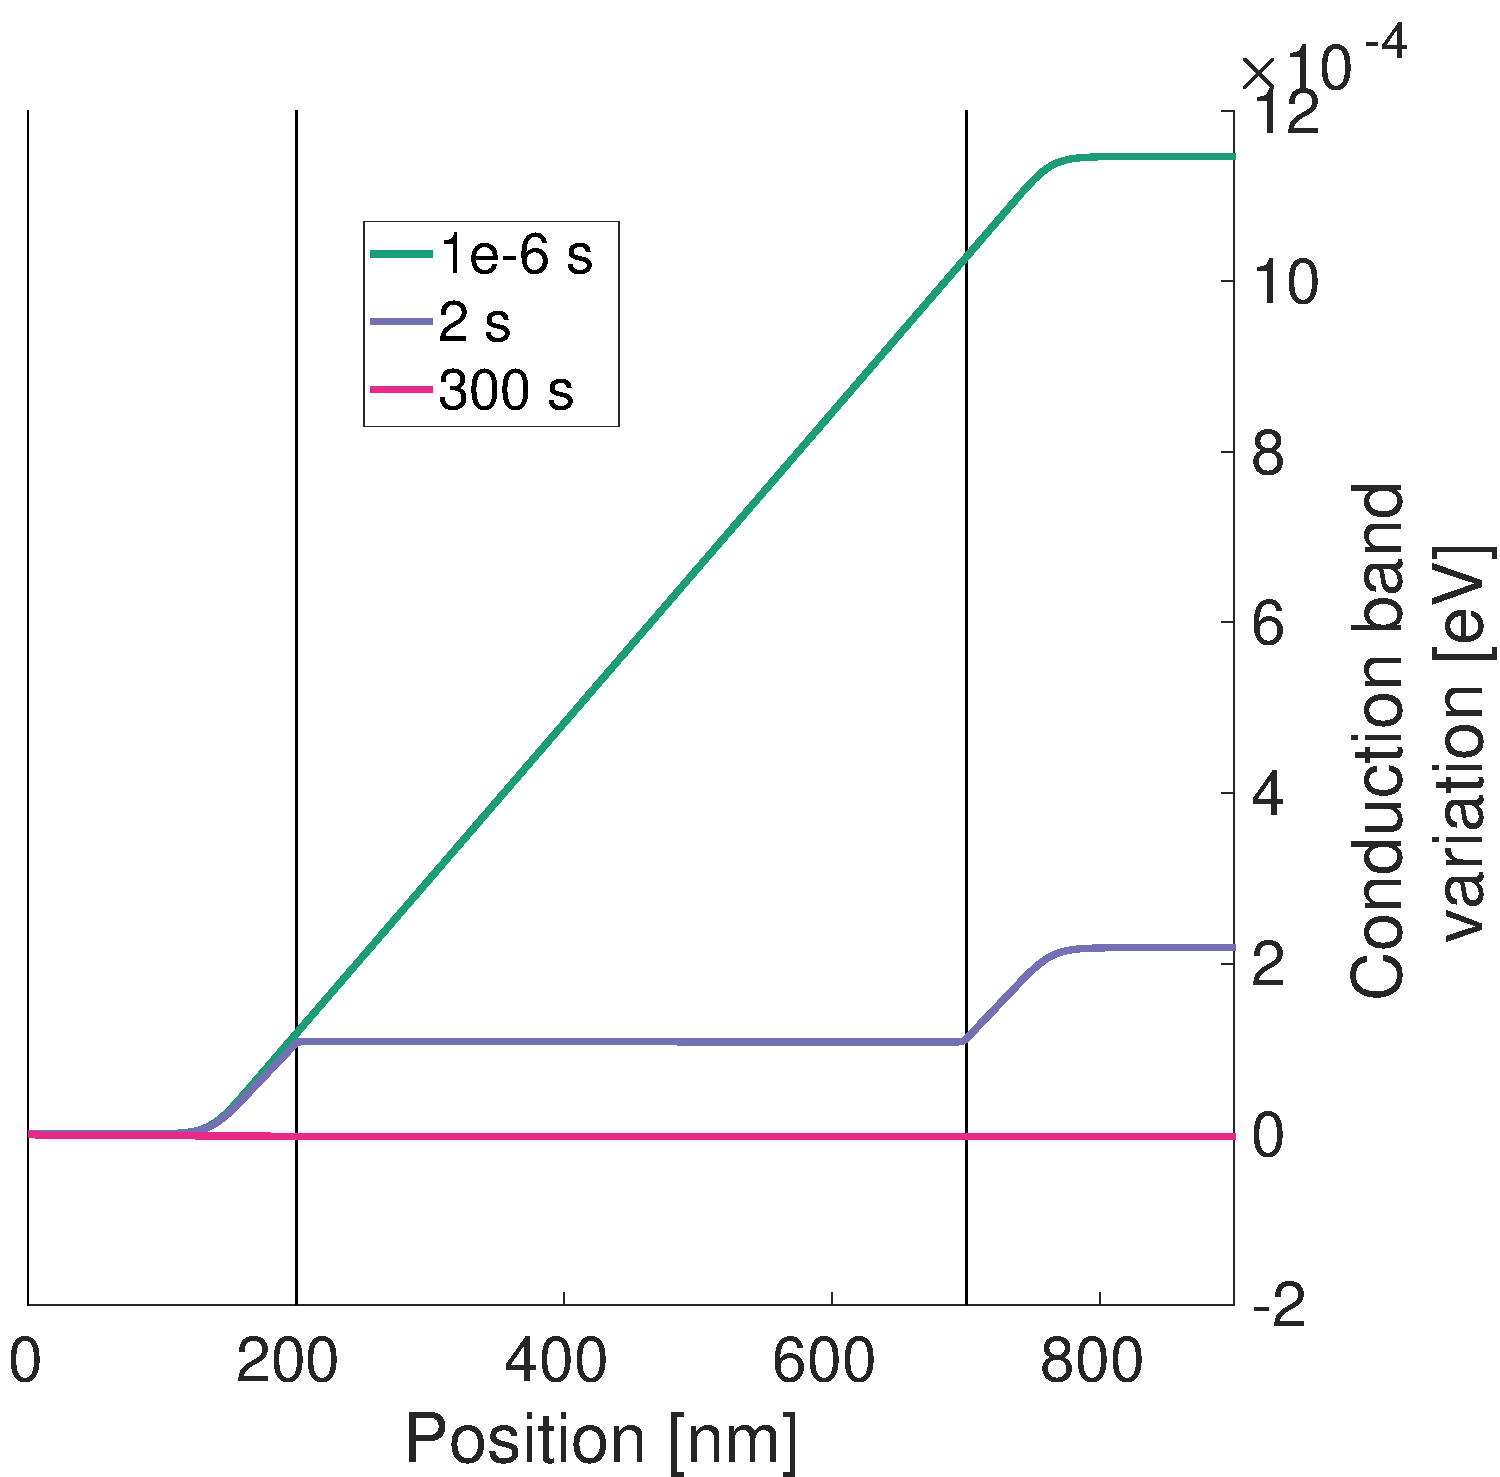
\includegraphics[width=0.9\textwidth]{tpv_ionic/tpv_ionic_cb.pdf}
				\subcaption{Conduction band \textit{variation} over time.}\label{fig:tpv_ionic-cb}
			\end{subfigure}
			\bigskip
			
			\begin{subfigure}[t]{1\textwidth}
				\centering
				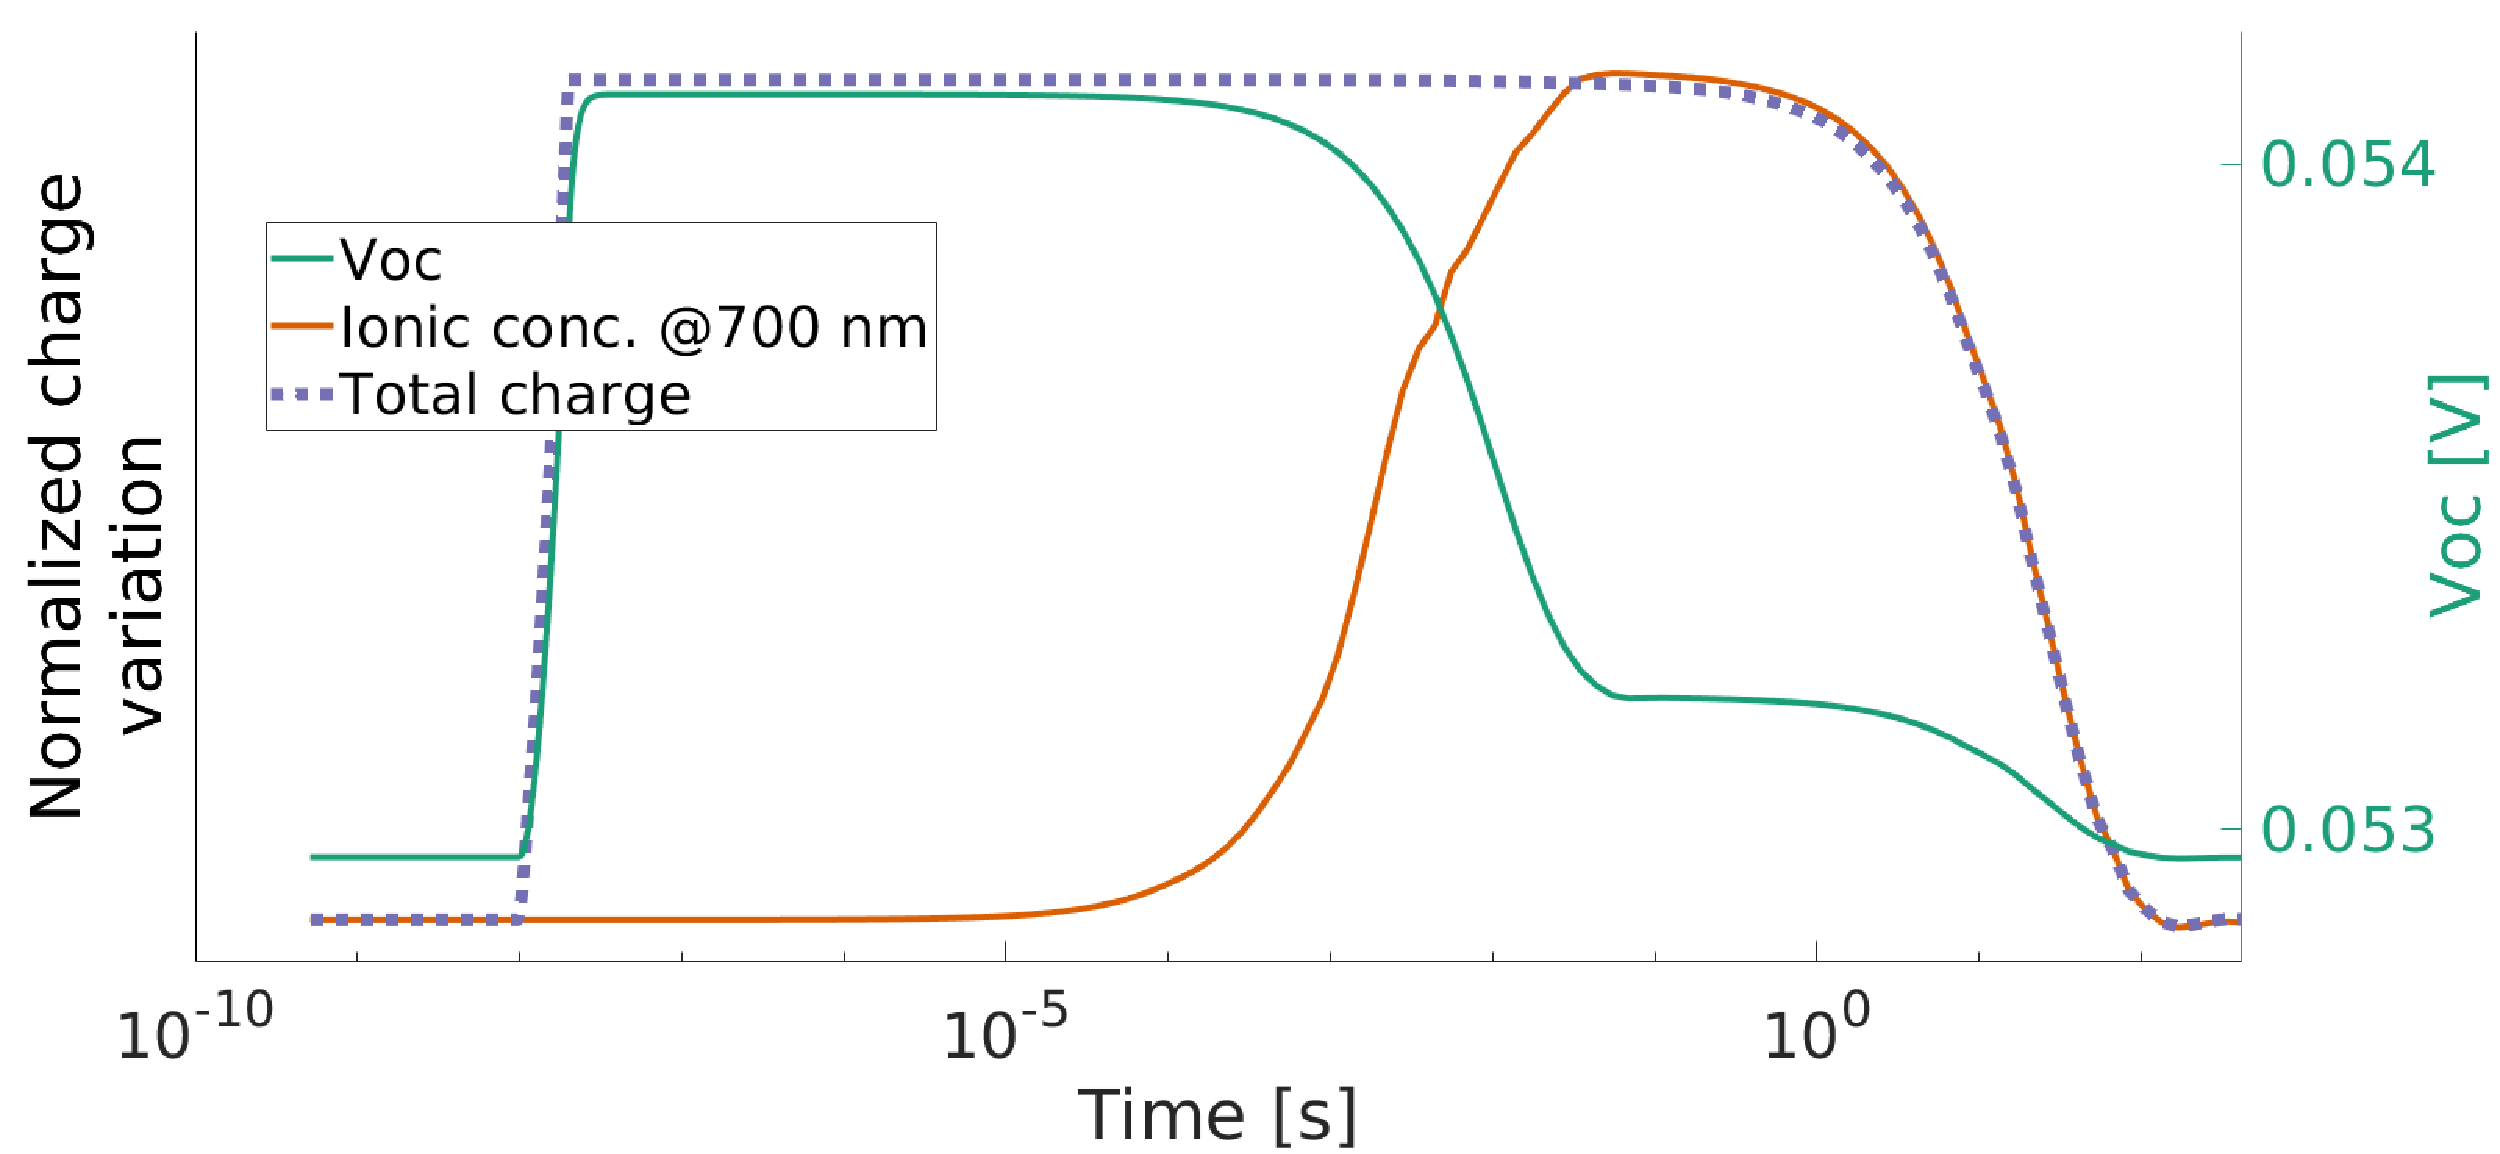
\includegraphics[width=0.8\textwidth]{tpv_ionic/tpv_ionic_dynamics.pdf}
				\subcaption{Voltage, charge, and ionic accumulation variation over time.}\label{fig:tpv_ionic-dynamics}
			\end{subfigure}
			\mycaption[Simulation of TPV at low background intensities with mobile ions.]{
				A TPV experiment has been simulated on a $p$(\SI{200}{\nm})--$i$(\SI{500}{\nm})--$n$(\SI{200}{\nm}) homojunction device with mobile ions in the absorber layer and at open circuit conditions.
				Low background light intensity \SI{1e-8}{suns} was applied, corresponding to a light bias of \SI{53}{\mV}.
				The illumination pulse was \SI{1e-8}{s} long and weak enough to cause a perturbation which can be considered small.
				In (\textbf{a}) the steady state energy levels and ionic profile is shown.
				In (\textbf{b}) the variation (the conduction band perturbation is too small for being plotted as in (\textbf{a})), taking the steady state profile as zero, of the conduction band during a TPV experiment.
				In (\textbf{c}), over time I plotted: the bi\hyp{}exponential voltage decay; the normalized total charge variation (the electronic profile integrated over the device thickness); and the ionic concentration variation at the perovskite/\gls{etm} interface, where the low ionic concentration temporarily increases during the transient.
				The represented data is interpreted in \cpageref{tpv_biexp_lowlight_ions}.
				\Gls{tpv} simulation routines explained in \cpageref{dd_tpv}.
			}\label{fig:tpv_ionic}
		}
	}
\end{figure}


		\paragraph{At low background illumination -- large perturbations}
		While bi\hyp{}exponential decays at high background illumination are often not observed, these are quite always present at lower background illumination, as in for the example reported in \cref{fig:tpv-biexp_full}.
		Clearly, the aforementioned explanation for bi\hyp{}exponential decays at high illumination are still valid for the low illumination case.
		Additionally, when studying a decay measured at very low background light intensity, we have to remember that we are out of the small perturbation regime and this could justify non\hyp{}exponential decays in various ways.
		In our simulation, we ensured to be in the small perturbation regime, still we observe bi\hyp{}exponential decays at low light biases as shown in \cref{fig:tpv_full_dd_ions}, so another explanation has to be found.

		\paragraph{At low background illumination -- ionic migration}\label{tpv_biexp_lowlight_ions}
		At low light intensity, the free carriers density can be very small, so that the recombination can be very slow.
		At these long times, another process of perovskite solar cells can be active: ionic migration.
		%	at the very long time scale of the recombination at low free carriers density (low background illumination)
		What we have observed, simulating a \acr{tpv} experiment on a homojunction device with mobile ions in the absorber layer, is that ionic profile can update to the pulse\hyp{}perturbed cell condition before the extra free charges recombine, in case this is very slow.
		In \cref{fig:tpv_ionic-reference} the steady state energy levels and ionic accumulation at the perovskite/contact interfaces is represented.
		In \cref{fig:tpv_ionic-cb} the variations of the conduction band profile are plotted.
		Here we can see that at \SI{1e-6}{s} the CB varies due to the new charges photo\hyp{}generated by the laser pulse, the non-flat conduction band indicates the presence of an electric field in the perovskite layer.
		At the same times, we can see in \cref{fig:tpv_ionic-dynamics} the increase in the total amount of electrons in the device due to the laser photo-generation which is reflected also by the open circuit voltage increase, as expected for a \acr{tpv} experiment.
		Then from \SIrange{1e-3}{1e-1}{s}, the ionic profile completely screens out the electric field.
		In \cref{fig:tpv_ionic-cb} this is visible as a flattening of the conduction band in the perovskite, this simple displacement of ions decreases the electrostatic potential at the \gls{etm}.
		In absence of changes in the charge density, a shift in the electrostatic potential in the \acr{etm} causes an identical shift in the quasi-Fermi levels in the \gls{etm}.
		As the voltage is defined as $V = \bar\mu_|CB|^{\mathrm{ETM}} - \bar\mu_|VB|^{\mathrm{HTM}}$ this shift clearly gets reflected in a voltage change.
		In the same time span, in \cref{fig:tpv_ionic-dynamics} we can see how the ionic concentration at an interface changes and how this gets reflected on the open circuit voltage, without any change in the total charge concentration.
		Finally, at longer times the laser\hyp{}generated free charges slowly recombine (the ionic profile just catches up this free charges variation), the CB returns to its steady state profile and a second decay is observed in the open circuit voltage.
		So, in this case, only the slow decay is actually related to charge recombination, while the fast one is due to the ionic profile update.
		%	This causes a first exponential decay of the voltage, followed by a second exponential decay due to the actual recombination of the charges generated by the laser pulse.
		This means that, if the simulation is correct, at low background light intensities we can obtain information on the ionic mobility and concentration from the fast component of bi\hyp{}exponential \acr{tpv} decays.
		%	The line at \SI{1e-6}{s} represents the CB just after the photo-generation of charges from the laser pulse; at \SI{2}{s} the ionic profile completely screened out the electric field; at longer times the generated free charges recombines and the CB returns to its steady state profile. 

		\begin{figure}
			\makebox[\textwidth][c]{
				\parbox{1.1\textwidth}{
					\centering
					\begin{subfigure}[t]{0.5\textwidth}
						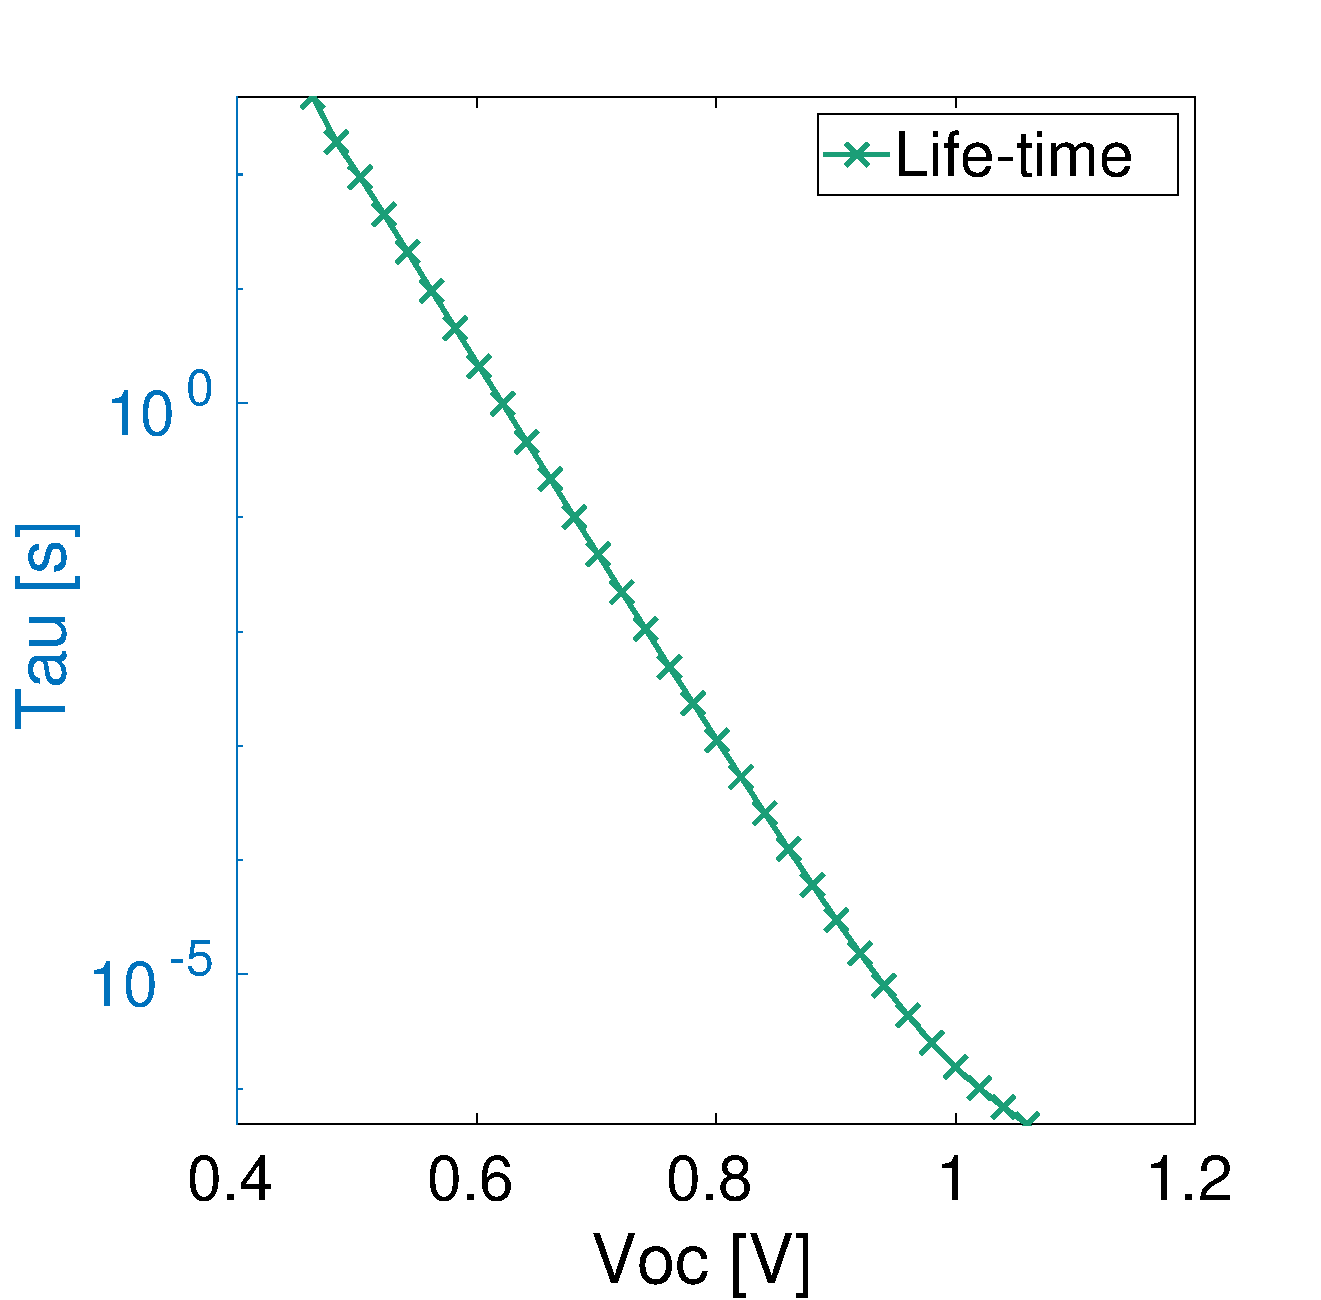
\includegraphics[width=1\textwidth]{tpv_full_dd/tpv_full_dd_noions.pdf}
						\subcaption{Without mobile ions, mono-exp.\ fit}\label{fig:tpv_full_dd_noions}
					\end{subfigure}
					\qquad
					\begin{subfigure}[t]{0.5\textwidth}
						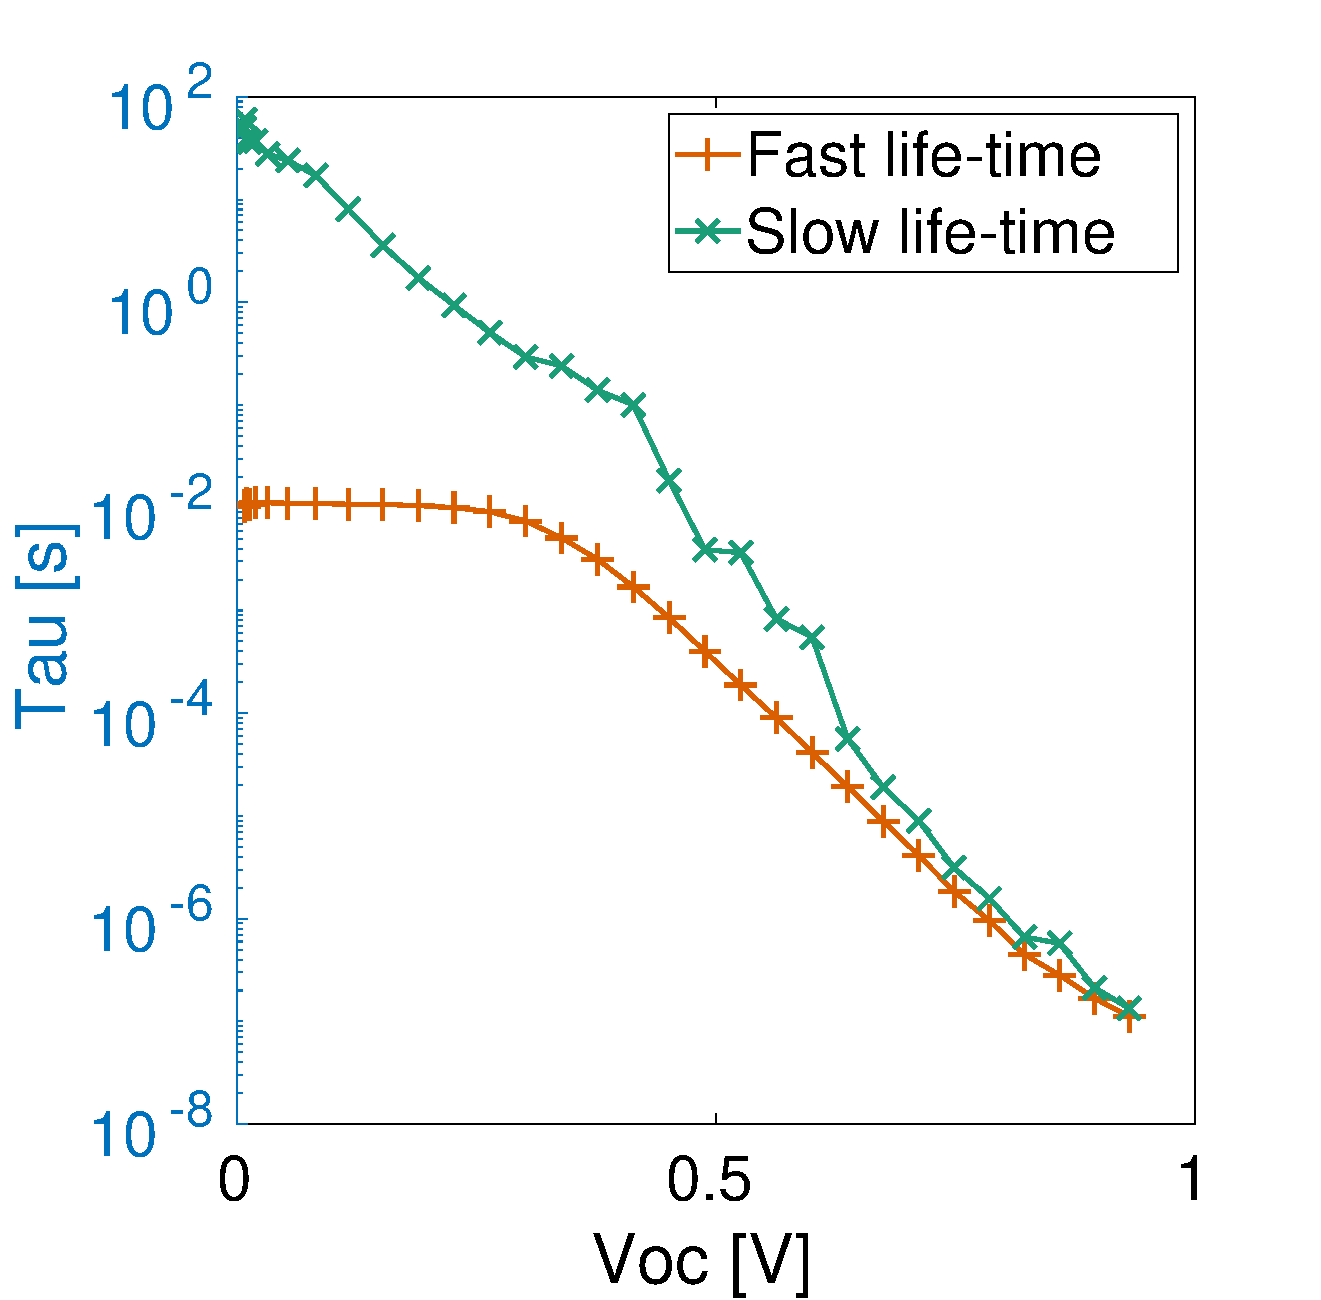
\includegraphics[width=1\textwidth]{tpv_full_dd/tpv_full_dd_ions.pdf}
						\subcaption{With mobile ions, bi-exp.\ fit}\label{fig:tpv_full_dd_ions}
					\end{subfigure}
					\mycaption[Simulated \glsentryshort{tpv} without and with mobile ions.]{
						The \acr{tpv} of a homojunction solar cell is simulated, with background illumination from \SIrange{1e-10}{1}{suns} (respectively the leftmost and the rightmost points) with 3 points per decade.
						The pulse intensity was regulated in order to not exceed \SI{8}{\mV} of perturbation.
						In (\textbf{a}) a device without mobile ions is simulated, the resulting decay is a simple exponential, so the lifetime of an exponential fit is reported.
						In (\textbf{b}) a device with mobile ions in the absorber layer is reported, the resulting decay is a simple exponential at high light biases but a bi\hyp{}exponential at lower background illuminations, so the two lifetimes from a bi\hyp{}exponential fitting are reported.
						\Gls{tpv} simulation routines explained in \cpageref{dd_tpv}.
					}\label{fig:tpv_full_dd}
				}}
		\end{figure}

		\paragraph{At low background illumination -- fast lifetime plateau}
		Both the fast and the slow component of bi\hyp{}exponential decays hit a maximum value (plateau) at very low light intensities.
		Looking at the fast component, assigned to the rearrangement of the ionic profile, we usually observe a constant lifetime.
		This suggests the presence of a background light insensitive ionic rearrangement time constant, which implies a light insensitive ionic mobility.
		This should be further studied considering the report of illumination-dependent ionic mobility by Maier's group in \authoryear{Kim2018}.
		
		\paragraph{At low background illumination -- calculating ionic resistance}
		We can consider this fast component's lifetime as a RC time due to ionic motion.
		So, from this time and from the ionic capacitance (easy to obtain from impedance spectroscopy, see \cpageref{impedance_lowf_dark}), we can obtain the ionic resistance (which is proportional to ionic mobility and to ionic concentration) as:
		\begin{equation}
			R_|ion| = \frac{\tau_|ion|}{C_|ion|}
		\end{equation}

		\paragraph{At low background illumination -- slow lifetime plateau}
		The slow decay component at very low background light intensity has been assigned to the electronic recombination.
		In drift-diffusion simulations, the lifetime does not show a maximum value and grows as the light intensity is decreased.
		But in the actual experiment setup, decays lifetimes are limited at long times by the discharge of the through the oscilloscope resistance and through the device shunt resistance, whatever is the fastest.
		This happens with an RC time of the circuit composed by the capacitance of the device (which can be obtained \textsl{via} a \acr{dc} experiment) and the \SI{1}{\Mohm} resistance of the oscilloscope or the internal device shunt resistance \cite{Tvingstedt2017}.
		The oscilloscope resistance could be varied using an attenuating probe (usually 10X or 100X) or a high impedance amplifier.
		This limit is often observed at low light intensities as a plateau in the \acr{tpv} lifetime \textsl{versus} light bias graph \cite{Tvingstedt2017}.
		Indeed, in \authoryear{Kiermasch2018}, where a \SI{1}{\tera\ohm} input impedance amplifier is used, the plateau is observable from \SIrange{1E-1}{1}{\s}, \textsl{i.e.}\ three orders of magnitude higher than what we observe with our \SI{1}{\Mohm} oscilloscope.
		This affirmation is corroborated by the correlation observable in \cref{fig:tpv_RCtime}.
		For mid-illumination intensities, the measured lifetime can be corrected considering the contribution from the RC time \cite{Credgington2014}.

		\begin{SCfigure}
			\centering
			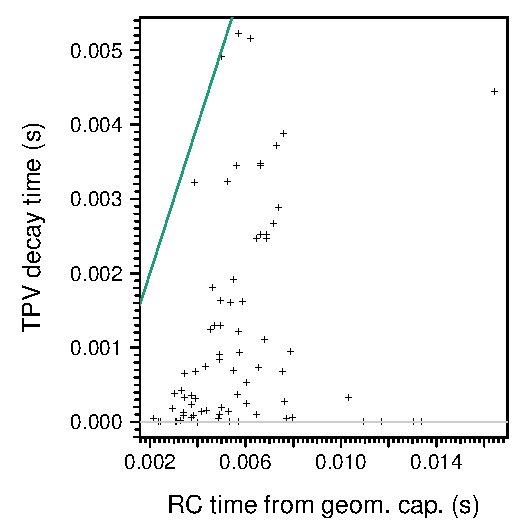
\includegraphics[width=0.5\textwidth]{tpv_RCtime/TPVdarkTime_vs_RCdarkTime.pdf}
			\mycaption[\Glsentryshort{tpv} time has an upper bond due to discharge through oscilloscope.]{
				Dark \acr{tpv} time (from a robust exponential fit) \textsl{versus} RC time derived from the geometric capacitance\index{geometric capacitance} from \acr{dc} and the \SI{1}{\Mohm} of the oscilloscope.
				Each point is a different device for a total of 76 devices, including many different structures.
				The green line indicates the 1 to 1 relationship.}\label{fig:tpv_RCtime}
		\end{SCfigure}

	\subsection{Interpretation of TPV \textsl{versus} Light Bias Trend}

		\paragraph{Lifetime \textsl{versus} light bias dependence}\label{tpv_tau_vs_intensity}
		Considering the small perturbation lifetime dependency from charge concentration due to a single dominant recombination mechanism from \cref{eq:tpv_tau_order} and substituting the charge with the expression for the charge from \cref{eq:ce_full} we can obtain a relation between the lifetime and the \gls{voc}.
		The main recombination mechanism in perovskite solar cells at open circuit conditions is the surface recombination (see \cpageref{intro_prv_recombination}) which, as described in \cpageref{intro_surface_recombination}, can be considered as a first\hyp{}order reaction with regards to the carriers \label{tpv_chemical_charge}in the perovskite layer.
		This carrier density is related to the chemical capacitance\index{chemical capacitance} represented as the exponential component in \cref{eq:ce_full}, so expanding $n_0$ from \cref{eq:tpv_tau_order} we obtain:
		%		For perovskite solar cells, the linear part of $n(V)$ related to the geometric capacitance\index{geometric capacitance} of charges accumulating in the selective contacts cannot be ignored and a discussion on whether to include it or not is needed.
		%	This "chemical" charge (charge stored in the perovskite layer) is represented as the exponential part of \cref{eq:ce_full}, so we obtain:
		\begin{dmath}\label{eq:tpv_tau_vs_intensity}
			\tau \approx (\Phi k n_0^{\Phi-1})^{-1} = \frac{n_|eq|^{1-\Phi}}{\Phi k} \left[\exp(\frac{q\voc}{mk_|B|T}) - 1\right]^{1-\Phi} \approx \frac{n_|eq|^{1-\Phi}}{\Phi k} \exp(-\frac{(\Phi-1)q\voc}{mk_|B|T}) = \frac{n_|eq|^{1-\Phi}}{\Phi k} \exp(-\frac{q\voc}{vk_|B|T}) = \frac{\tau_0}{\Phi} \exp(-\frac{q\voc}{vk_|B|T})
		\end{dmath}
		where we used that $qV \gg k_|B|T$ for all non-dark cases in order to neglect the $-1$ addend.
		The pre\hyp{}factor $\tau_0 = n_|eq|^{1-\Phi}/k$ represents the thermal equilibrium lifetime.
		As shown, the lifetime typically decreases exponentially with the light bias, as experimentally observed in the example of \cref{fig:tpv-monoexp}, with an ideality modifier of $v = m/(\Phi-1)$.
		This relation is in accordion with equivalent studies on \gls{osc} \cite{Shuttle2008,Shuttle2008d,Credgington2011}.

		\paragraph{Diode\hyp{}capacitor discharge could be the limiting time}
		Similarly to the example we just considered, where RC times put a cap to the slow observable lifetimes, \authoryear{Kiermasch2018} underlines that also the often-neglected diode\hyp{}capacitor discharge could have the same effect \cite{Tvingstedt2017,Hellen2003}.
		The relevant capacitance would be the geometric capacitance\index{geometric capacitance} of the generated charges accumulating in the depletion\index{space charge layer} layers and the diode would be the perovskite-contacts interfaces with the relative dark saturation current.
		Basically this represents a re\hyp{}injection of the majority charges from the contacts back to the perovskite, this causes a voltage decrease without actually needing recombination: charges could just diffuse back.
				The lifetime observed in this regime would also decrease exponentially with the light bias \cite{Castaner1981}.
				In his PhD thesis, also \authoryear{Calado2018} observed and modelled this effect, named "thermionic emission".
				All the authors agree that this effect is more important at low light intensity for thin devices (high capacitance) \cite{Kiermasch2018} while it could be negligible at high background illuminations.
		Also when performing full signal Open Circuit Voltage Decay dynamics measurement (OCVD) \cite{Lederhandler1955,Mahan1981}, which has not been performed in this thesis, this limitation has to taken in consideration \cite{Tvingstedt2017,Pockett2017,Pockett2015,Kiermasch2018}.

		\FloatBarrier
		\newpage
		\mysection[TPV-CE]{Transient PhotoVoltage Referenced to Charge Density (TPV-CE)}\label{characterization_tpvce}

		\paragraph{Concept}
		This is a meta experiment which combines the data from \acr{tpv} and \acr{ce} without needing any additional experimental step.
		Joining the information about charge lifetime \textsl{versus} light bias from \acr{tpv} with the information about charge density \textsl{versus} light bias from \acr{ce}, we obtain the relation of the charge lifetime \textsl{versus} charge density.
		This new relationship is more useful than the results from bare \acr{tpv}, as it allows us to make a fair comparison between different devices.

		\paragraph{Procedure}
		The voltage dependency of the small perturbation lifetime $\tau(V)$ obtained from \acr{tpv} gets expanded with the $V(n)$ relation which can be obtained inverting the fitted function of $n(V)$ from a \acr{ce} experiment for obtaining a $\tau(n)$ relation.
		A reaction order $\Phi$ can be obtained fitting the $\tau(n)$, this can be used for correcting the small perturbation lifetime to obtain a pseudo first order lifetime \textsl{i.e.}\ total carrier lifetime $\tau_|pfo|(n)$ which can be compared between devices with different recombination mechanisms.

		\paragraph{Which charge from \glsentryshort{ce}}
		In \gls{osc} literature, where a simple exponential charge \textsl{versus} voltage is usually observed, the full $n$ obtained by \acr{ce} is taken.
		In perovskite solar cells, the charge from chemical capacitance\index{chemical capacitance} is usually considered as the relevant charge density for surface recombination, as explained in \cpageref{tpv_chemical_charge}, so just the exponential addend is taken from the fit of \acr{ce} data performed with \cref{eq:ce_full} \cite{Du2018,Gelmetti2019,Wheeler2017}.
		As a reference, the \cref{fig:tpvce-full,,fig:tpvce-nogeom} can be compared where the full charge from \acr{ce} is employed in the former while just the charge from chemical capacitance\index{chemical capacitance} was used for the latter.
		Using \cref{eq:tpv_tau_order} for fitting the data, we can obtain physically unreasonable recombination orders when considering the full charge from \acr{ce} (reported in \cref{fig:tpvce-full}).
		%, with the same ordering of the legend respectively $5.4$, $3.2$, $9.8$, and $16.0$).
		Instead, fitting data with the exponential component of \acr{ce} only, the recombination orders obtained are between 1 and 2, which are the expected values (reported in \cref{fig:tpvce-nogeom,,fig:tpvce-nogeom_total}).
		% with the same ordering of the legend, respectively $1.6$, $1.5$, $1.9$, and $1.8$).
		%  information on the recombination processes, it is more useful to relate the recombination lifetime to the charge concentration, rather than to the light bias, as in a pure \acr{tpv} experiment.
		%	One way to obtain this is taking the $\tau (V)$ relation from \acr{tpv} and substituting $V$ with the inverse of $n(V)$ obtainable from \acr{ce} experiments, obtaining the $\tau (n)$ relationship.
		%	For perovskite solar cells, the linear part of $n(V)$ related to the geometric capacitance\index{geometric capacitance} of charges accumulating in the selective contacts cannot be ignored and a discussion on whether to include it or not is needed.
		%	In this thesis recombination order $\Phi = \lambda + 1$  AAAAAAAAAAAAAAAAAAAAAAAAAAAAAA

		\begin{figure}
			\makebox[\textwidth][c]{
				\parbox{1.1\textwidth}{
					\centering
					\begin{subfigure}[t]{0.5\textwidth}
						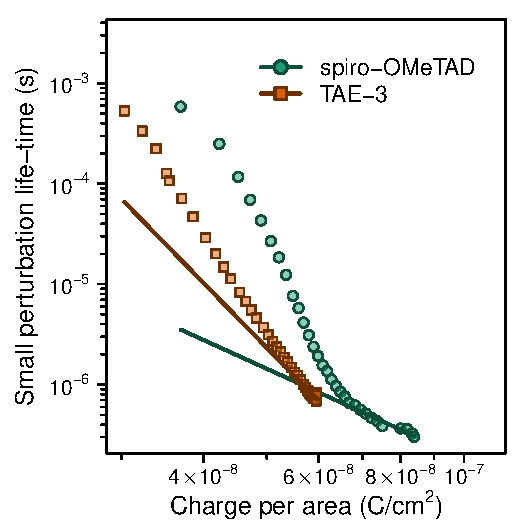
\includegraphics[width=1\textwidth]{tpvce/spiro_vs_TAEs-TPVCEs.pdf}
						\subcaption{Full charge from \acr{ce}}\label{fig:tpvce-full}
					\end{subfigure}
					\bigskip

					\begin{subfigure}[t]{0.5\textwidth}
						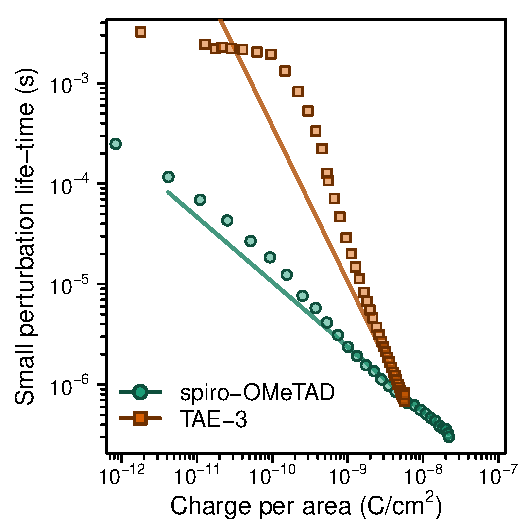
\includegraphics[width=1\textwidth]{tpvce/spiro_vs_TAEs-TPVCEs-nogeom.pdf}
						\subcaption{Exp.\ charge from \acr{ce}}\label{fig:tpvce-nogeom}
					\end{subfigure}
					\qquad
					\begin{subfigure}[t]{0.5\textwidth}
						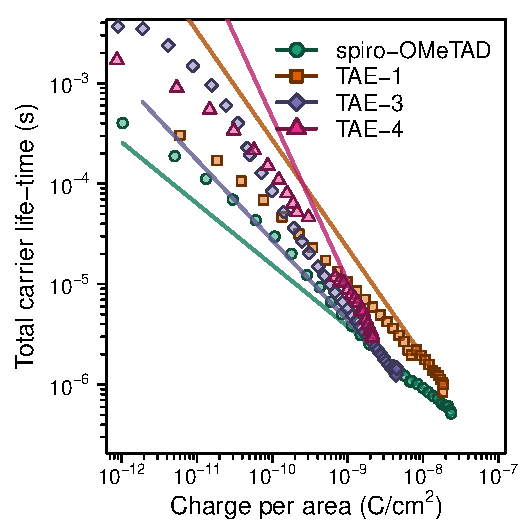
\includegraphics[width=1\textwidth]{tpvce/spiro_vs_TAEs-TPVCEs-nogeom_total.pdf}
						\subcaption{Exp.\ charge from \acr{ce} and lifetime corrected with $\Phi$}\label{fig:tpvce-nogeom_total}
					\end{subfigure}
					\mycaption[Example of TPV-CE processed in different ways.]{
						Solid lines are the power-law fit with the formula $y = k^{-1} x^{1-\Phi}$.
						In (\textbf{a}) the charge used for the independent variable is taken from the full charge extracted in the \acr{ce} experiment, including the charge stored in contacts and electrodes.
						The $\tau_|pfo|$ lifetime as obtained from \acr{tpv} is used as dependent variable.
						In (\textbf{b}) just the charge from chemical capacitance\index{chemical capacitance} (exponential addend in \cref{eq:ce_full}) is used as independent variable.
						In (\textbf{c}) the $\tau$ is corrected using the fitted recombination order $\Phi$ to obtain the total carriers lifetime $\tau_|pfo| = \Phi\tau$.
						Data from \gls{fto}\-/\ch{d-TiO2}\-/\gls{csfamapbibr}\-/\gls{htm}\-/\ch{Au} solar cells \cite{Gelmetti2019}.
					}\label{fig:tpvce}
				}
			}
		\end{figure}

		\paragraph{From small perturbations lifetime to rate constant -- first\hyp{}order reaction}
		Here we consider a simple case where just a first order or a second order recombination is present.
		From the \cref{eq:tpv_tau_order} it is clear that for the first\hyp{}order reaction case it is easy to obtain $k_1 = \tau^{-1} = \tau_|pfo|^{-1}$.
		One fact of \cref{eq:tpv_tau_order} for the $\Phi=1$ case have to be underlined: the small perturbations lifetime for a first\hyp{}order recombination does not depend on the charge density, so it would appear as a plateau in the lifetime \textsl{versus} charge plot \cite{Kiermasch2018} which is not usually experimentally observed.

		\paragraph{From small perturbations lifetime to rate constant -- higher order reaction}
		For the second and higher order recombination cases, to obtain $k$ is non\hyp{}trivial as it is related to $\tau$ \textsl{via} the charge density \cite{ORegan2007} and the reaction order \cite{Shuttle2008,Du2018,Barnes2011,Barnes2011a} as shown in \cref{eq:tpv_tau_order}.
		From this equation we can notice that correcting the small perturbation lifetime $\tau$ we can easily obtain a pseudo first order lifetime (total carrier lifetime) $\tau_|pfo|$ as:
		\begin{equation}\label{eq:tau_pfo}
			\tau_|pfo| = \Phi \tau = k^{-1} n_0^{1-\Phi}
		\end{equation}
		where $n_0$ is the excess carriers in the device.
		This simple correction allows us to make a meaningful graphical comparison between recombination rates at a given charge density, as represented in \cref{fig:tpvce-nogeom_total}.
		The units of recombination constant $k$ are rather unusual: \si{\s^{-1}.\cm^{2\Phi-2}}.
		In order to obtain a more useful value, the lifetime extrapolated at zero applied voltage $\tau_0=n_|eq|^{1-\Phi}/k$ is often employed \cite{Kirchartz2012,Du2018,Kiermasch2019,Wheeler2017} (as already used in \cref{eq:tpv_tau_vs_intensity}):
		\begin{equation}\label{eq:tau_pfo_neq}
			\tau_|pfo| = \tau_0 \left(\frac{n_0}{n_|eq|}\right)^{1-\Phi}
		\end{equation}
		where $n_|eq|$ is the chemical capacitance\index{chemical capacitance} prefactor obtained from \cref{eq:ce_full} indicating the intrinsic carrier density at equilibrium.

		%Because of this, when an information on underlying rate constants is sought, comparisons of $\tau_|pfo|$ have been performed taking care of having similar charge densities in the devices under study \cite{ORegan2008}, \textsl{i.e.}\ comparing vertically (points at the same charge density) in \cref{fig:tpvce}.
		%\paragraph{Obtaining the recombination reaction order}
		%As shown in \cref{eq:tpv_tau_order}, we can extract the reaction order from a power-law fitting of the $\tau_|pfo|$ \textsl{versus} $n$ from chemical capacitance\index{chemical capacitance} data.

		\FloatBarrier
		\newpage
\section{Transient PhotoCurrent (\glsentryshort{tpc})}\label{characterization_tpc}

	\begin{SCfigure}
		\centering
		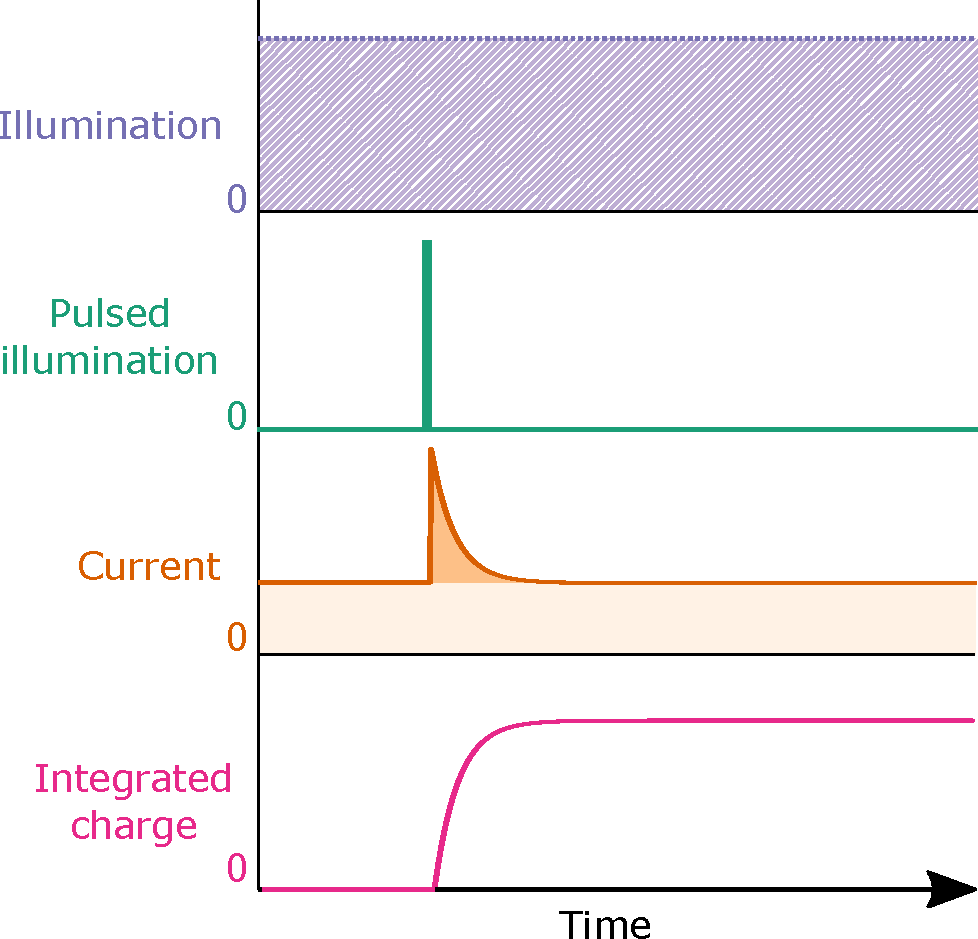
\includegraphics[width=0.65\textwidth]{tpc_scheme/tpc_scheme2.pdf}
		\mycaption[Scheme of TPC experiment.]{
			A device is illuminated while short circuited through a small resistance, then a short light pulse is added and the additional flowing current is integrated to give the photo\hyp{}generated charge. The constant illumination intensity is changed and the measurement is repeated.}\label{fig:tpc_scheme}
	\end{SCfigure}

	\paragraph{Concept}
	This technique, applied to a solar cell at short circuit conditions, allows us to study the dependence of \gls{eqe} on the light illumination intensity \cite{ORegan2004}.
	It gives approximatively the same information of the \gls{jsc} \textsl{versus} light intensity experiment explained in \cpageref{jsc-phi}.
	Usually, the actual value of \gls{eqe} (generated charge over incident photons ratio) is not calculated, rather just the generated charge amount $\Delta n$ for a given laser pulse intensity in measured.
	%, rather than actual value of \gls{eqe} (generated charge over incident photons ratio) is obtained as the incident power is not usually measured (on the contrary to the classical \gls{eqe} experiment).

	\begin{SCfigure}
		\centering
		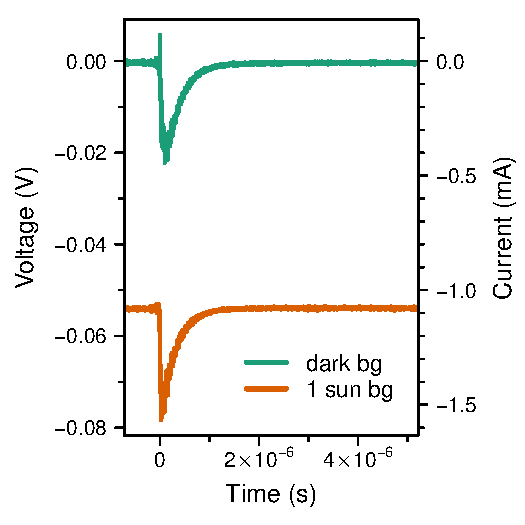
\includegraphics[width=0.5\textwidth]{tpc/tpc_vs_tpc-TAE-4_ig101-1555-1.pdf}
		\mycaption[Example of TPC experiment at dark and 1 sun background illumination.]{
			The current profile of a \gls{fto}\-/\ch{d-TiO2}\-/\gls{csfamapbibr}\-/\gls{tae4}\-/\ch{Au} solar cell \cite{Gelmetti2019} short circuited through a small resistance either in dark or illuminated with \SI{1}{sun} and perturbed with a laser pulse.
			The voltage axis can easily be converted to the current axis dividing by the known small resistance of \SI{50}{\ohm}.
			The integrated peak resulted in \SI{0.17}{\nano\coulomb} for the dark case and \SI{0.14}{\nano\coulomb} for the \SI{1}{sun} one.
		}\label{fig:tpc}
	\end{SCfigure}

	\paragraph{Procedure}
	The device is short circuited through a \SI{50}{\ohm} resistor and kept either at dark or under 1~sun illumination by a white \gls{led} ring until stabilisation is reached.
	Failure to reach stabilisation of the ionic profile will affect the measurement results \cite{Belisle2017}.
	Then, as represented in \cref{fig:tpc_scheme}, an additional illumination pulse is provided \textsl{via} a nitrogen laser and the voltage across the \SI{50}{\ohm} resistor is monitored using an oscilloscope connected in parallel.
	%	The signal is acquired by an oscilloscope in parallel to the \SI{50}{\ohm} resistor.
	This allows us to measure a potential drop across the resistor and to obtain the related current \textsl{via} Ohm's law $J = V / R$.
	Subtracting the constant current due to the background illumination and integrating the transient over time gives the charge photo\hyp{}generated by the laser pulse.
	This process is repeated at 1~sun and at dark background illumination conditions, as shown in \cref{fig:tpc}.
	For each illumination intensity, the reported decay is the result of averaging around 30 transients in order to increase the signal to noise ratio.
	1~sun equivalent illumination is defined as the illumination at which a silicon photodiode gives the same \gls{jsc} as under calibrated 1~sun from the solar simulator.

	\paragraph{Small resistance and fast extraction}
	The characteristic time of a \acr{tpc} decay is often comparable with the small perturbation lifetime from \acr{tpv} experiment at high background illumination.
	This not necessarily invalidate the \acr{tpc} result, as the slow time could be due to the slow transport in the selective contacts.
	The \acr{tpc} time can be limited by the RC time constant of the extracting circuit, in case a faster extraction is needed, a smaller resistance can be employed (clearly, the measure will be more noisy).
	Thanks to the short time of the measurement, both with or without background illumination, we can assume that the ionic migration is never observed in this measurement.

	\paragraph{Dependency on background illumination}\label{tpc_intensity}
	When measuring \acr{tpc} at various background illumination intensities, a constant pulse\hyp{}generated charge amount can be gathered for low illuminations that starts decreasing as the background illumination exceeds \SI{1}{sun} (as reported for perovskite solar cells in fig.~S5 of \cite{Du2018} and partially in fig.~S9 of \cite{Wheeler2017}).
	In \gls{osc} this was assigned to primary geminate recombination, which, as seen in \cpageref{intro_geminate}, is negligible in perovskite materials.
	The influence of the different electric field intensity on the absorption, explained in \cpageref{software_electroabsorbance}, can be neglected as the field is screened in most of the absorber and anyway the electro\hyp{}absorbance phenomena (Franz\hyp{}Keldysh effect) should have just a small contribution.
	Other kind of recombination can affect the extracted charge, even in short circuit conditions, if the charge extraction is not sufficiently quick.
	For this reason, in case of large discrepancies between the dark and the \SI{1}{sun} background illumination measures, the dark one better describes the photo\hyp{}generated free\hyp{}charge (in case the dark and illuminated results were different, the first quartile of all \acr{tpc} measurements was used).

	\FloatBarrier
	\newpage
\section{Differential Capacitance (DC)}\label{characterization_dc}

	\paragraph{Concept}
	\Acr{dc} is a meta-measurement as it just combines the data from \acr{tpv} and \acr{tpc} without requiring any additional experimental step \cite{ORegan2005,ORegan2006,Shuttle2008,Credgington2014,Maurano2011}, sometimes also referred to as "differential charging".
	From \acr{tpc} we obtain how much charge $\Delta n$ has been generated by the laser pulse and from \acr{tpv} we obtain the voltage increase $\Delta V$ due to the additional charge.
	Relating these two quantities, \acr{dc} allows us to measure the capacitance of the solar cells at different light biases.
	%	we can obtain a light bias dependent capacitance.
	Integrating this capacitance profile over voltage we can obtain the extra charge density \textsl{versus} light bias profile.
	This information is equivalent to the results from \acr{ce}, with the advantage that this technique is a small perturbation technique, working on a stabilised device around its steady state conditions.
	Differently to \acr{ce}, \acr{dc} is an intrinsically short time\hyp{}scale technique in which the ionic migration should never be observed.
	This technique has also been used for estimating the electronic band gap of the perovskite layer in \authoryear{Wheeler2017,Credgington2014}, considering that also for \acr{dc} as seen for \acr{ce} in \cpageref{ce_energy_levels}, the exponential trend is expected to gain importance as the quasi-Fermi splitting approaches the built-in voltage.
	For \gls{osc}, the consistency of this observation has been validated using \gls{ups} in \authoryear{Credgington2014}.

	%	\begin{equation}C(V') = \left.\frac{dn}{dV}\right\rvert_{V=V'}\end{equation}
	%	This allows us to estimate the capacitance of the solar cell device at open circuit with various illumination intensities.

	\paragraph{Procedure}
	The laser pulse intensity has to be the same for the \acr{tpc} and the \acr{tpv} experiments.
	The needed value of $\Delta V$ is the \gls{voc} increase due to the laser pulse, prior to the decay to steady state, for each illumination intensity.
	The amount of charge photo\hyp{}generated by the laser pulse $\Delta n$ is obtained from \acr{tpc}.
	In order to use the charge measured in \acr{tpc} at short circuit for referencing the data from \acr{tpv} at open circuit we have to assume that $\Delta n$ is the same at open and short circuit conditions.
	In other words, we assume that the \gls{eqe} does not depend on the applied voltage.
	Additionally, we have to assume that the \gls{eqe} does not depend neither on the background illumination intensity for a device at open circuit conditions (used for \acr{tpv}).
	This point was discussed for \acr{tpc} in \cpageref{tpc_intensity}.
	%	he   the same assumption done for \acr{tpc} and explained in \cpageref{tpc_intensity}: the charge generation (\gls{eqe}) is independent from background light illumination.
	%	We assume that the \gls{eqe} is the same at short and open circuit conditions, which means: the charge measured in \acr{tpc}, at short circuit, will be used for referencing data from \acr{tpv}, at open circuit.
	Adapting the definition of capacitance "the ratio of the change in an electric charge in a system to the corresponding change in its electric potential" \cite{WikipediaCapacitance2019} to an applied voltage dependent capacitance, we can write:
	\begin{equation}\label{eq:dc}
%		C(V') = \eval{\dv{n}{V}}_{V=V'}
		C(V) = \eval{\frac{\Delta n}{\Delta V'}}_{V'=V}
	\end{equation}
	where $C$ is a light bias $V$ dependent capacitance, $n$ is the perturbed electron density, and $V'$ is the perturbed voltage.
	So, the charge obtained from the \acr{tpc} experiment is divided by an array of voltage increases $\Delta V'(V)$ values obtained from \acr{tpv}, one for each illumination intensity.
	The obtained capacitance value is plotted versus the steady state light bias $V$.
	The capacitance can be integrated over voltage for obtaining a charge density \textsl{versus} light bias relationship:
		\begin{equation}\label{eq:dc_charge}
	n_|DC|(V) = \int_{0}^{V} C(V') \dd V'
	\end{equation}
	\paragraph{Capacitance dependence on applied voltage}
	The electrical capacitance of most of the commercial capacitors is independent on the applied voltage, as represented in \cref{fig:cap_voltage_dependence_commercial} where the capacitance was measured with a modified \acr{ce} experiment where the pre\hyp{}conditioning was done directly applying a voltage instead of applying a light bias.
	This means that the extracted charge is linearly proportional to the applied voltage.
	On the contrary, the electrical capacitance of a solar cell does depend on the applied voltage or light bias, as shown in \cref{fig:cap_voltage_dependence_tae1}.
	\begin{figure}%[!hbtp]%
		\makebox[\textwidth][c]{
			\parbox{1.1\textwidth}{
				\centering
				\begin{subfigure}[t]{0.5\textwidth}
					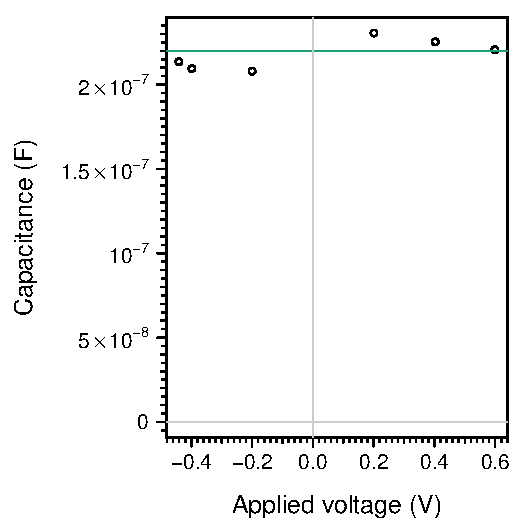
\includegraphics[width=0.9\textwidth]{cap_voltage_dependence/reference220nF/reference220nF.pdf}
					\subcaption{Commercial \SI{220}{\nano\F} capacitor.}\label{fig:cap_voltage_dependence_commercial}
				\end{subfigure}
				\qquad
				\begin{subfigure}[t]{0.5\textwidth}
					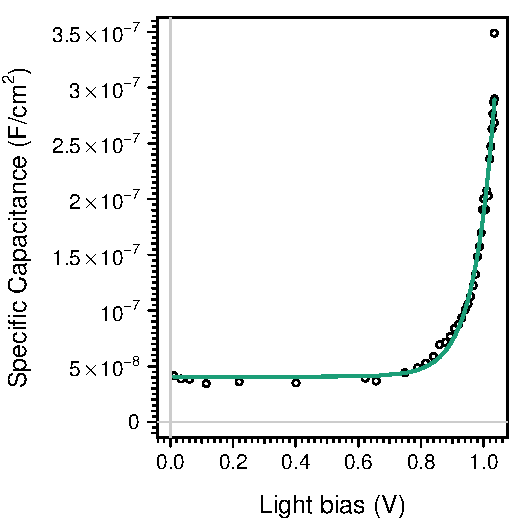
\includegraphics[width=0.9\textwidth]{cap_voltage_dependence/TAE-1_ig94-1559-1/DC-capacitance-TAE-1_ig94-1559-1.pdf}
					\subcaption{Perovskite solar cell.}\label{fig:cap_voltage_dependence_tae1}
				\end{subfigure}
				\mycaption[Capacitance dependence on applied voltage.]{
					In (\textbf{a}) the capacitance of a commercial capacitor is reported, it was measured using \acr{ce} with applied voltage bias instead of the classical light bias used for solar cells.
					The capacitance is obtained as the extracted charge over the applied voltage prior to short circuiting.
					In (\textbf{b}) the typical capacitance \textsl{versus} voltage profile of a \gls{fto}\-/\ch{d-TiO2}\-/\gls{csfamapbibr}\-/\gls{tae1}\-/\ch{Au} device \cite{Gelmetti2019} is shown as measured by \acr{dc}.
					In this case the indicated voltage is originated by various illumination intensities at open circuit prior to short circuiting.}\label{fig:cap_voltage_dependence}
			}}
	\end{figure}

	\paragraph{Small perturbations}\label{dc_perturbation}
	As mentioned in \cpageref{tpv_perturbation}, we measure \acr{tpv} ensuring to be in the small perturbation conditions for high light bias illumination.
	But the perturbations are surely large getting close to dark illumination conditions.
	This happens because we are not changing the laser pulse intensity when decreasing the background illumination.
	This way, we can measure just one \acr{tpc} for knowing the amount of generated charge, as we assume that it depends just on the laser pulse intensity.
	The measure of as many \acr{tpc} as many laser pulse intensities would be too complex with our current experimental setup.

	\paragraph{Consideration on mobility limited case}
	In order to have a meaningful voltage peak value, the charges have to equilibrate with the cell electrodes quickly compared to the recombination rate \cite{Credgington2014}.
	In a mobility limited case, as explained in \cpageref{tpv_mobility}, the charges could recombine so quickly that the $\Delta V$ value could be underestimated.

	\paragraph{Voltage peak value from \glsentryshort{tpv}}\label{tpv_deltaV}
	The $\Delta V$ value can be obtained in various ways, the following methods were tested:
	\begin{itemize}
		\item The maximum voltage point, subtracting the steady state \gls{voc} (\cref{fig:dc_deltaV-deltaV}). This is the classical way to obtain $\Delta V$ but it is heavily affected by the aforementioned noise when a short time window is used.
		\item The linear factor $\Delta V$ in an exponential fit $V (t) = V_0 + \Delta V \cdot e^{-t/\tau}$ was used, but it can fail if the decay does not have a simple exponential shape (often a bi\hyp{}exponential is observed, \cref{fig:dc_deltaV-monoexp}).
		\item In cases where the \acr{tpv} decays have a bi\hyp{}exponential behaviour, the sum of the two linear factors $\Delta V = \Delta V_a + \Delta V_b$ in a bi\hyp{}exponential fit as in \cref{eq:tpv_biexp} could improve the previous method (\cref{fig:dc_deltaV-biexp}). One have to carefully set boundary values to the fitting parameters for avoiding a fast exponential matching just some noise.
		\item The maximum value of a \gls{loess} local regression was used, but this underestimates the value, especially when the peak top are just few points (when the measurement time window is large, \cref{fig:dc_deltaV-loess}).
		\item The average of the values registered starting from the maximum voltage point and during a specified time lapse. For selecting the maximum voltage without interferences from the noise, a custom smoothing function is used (\cref{fig:dc_deltaV-firstPoints}).
	\end{itemize}
	This last option is the one used in this thesis.
	The average was performed over \SI{50}{\nano\s} after the peak and this allowed us to get a reliable $\Delta V$ value.
	As an example, we can compare the $\Delta V$ obtained with the aforementioned criteria applied on the \acr{tpv} decay in \cref{fig:tpv_robust}: \SI{16.5}{\mV} from the maximum point; \SI{4.2}{\mV} from the simple mono\hyp{}exponential fit; \SI{3.3}{\mV} from the robust mono\hyp{}exponential fit ; \SI{5.9}{\mV} from the simple bi\hyp{}exponential fit; \SI{6.1}{\mV} from the robust bi\hyp{}exponential fit (see \cpageref{tpv_robust} for discussion on robust fitting); \SI{4.2}{\mV} from the maximum of the \gls{loess}; \SI{4.6}{\mV} using the average of the first points after the peak.
	To further illustrate the sensibility of \acr{dc} from the $\Delta V$ estimation, the capacitance of four devices from \cite{Gelmetti2019} has been reported in \cref{fig:dc_deltaV}.
	If the object of study is related to the presence of negative peaks, present in non-stabilised solutions as described in \cpageref{tpv_negativePeaks}, the data fitting code should be modified.
	A non stabilised ionic profile during the \acr{tpv} measurement can lead to shifts in the \acr{dc} profile \cite{ORegan2015b}.
	The biphasic behaviour of \acr{tpv} decays at low background intensity due to ionic migration, discussed on \cpageref{tpv_biexp_lowlight_ions}, does not reduce the validity of the $\Delta V$ value for capacitance determination, as at very short times the ionic profile is effectively frozen.

	\begin{figure}
		\makebox[\textwidth][c]{
			\parbox{1.1\textwidth}{
				\centering
				\begin{subfigure}[t]{0.5\textwidth}
					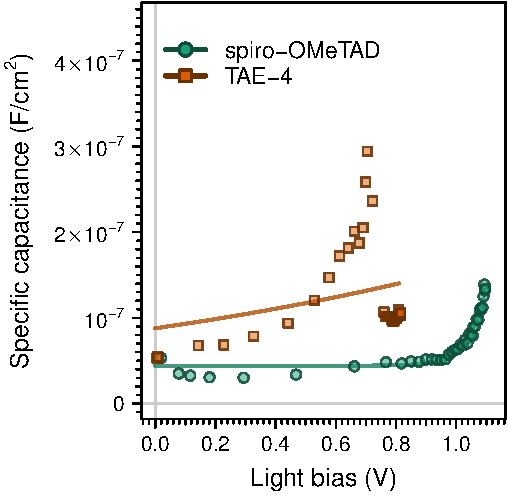
\includegraphics[width=0.75\textwidth]{dc_deltaV/deltaV-spiro_vs_TAEs-DCs-capacitance-crop.pdf}
					\subcaption{Maximum voltage point}\label{fig:dc_deltaV-deltaV}
				\end{subfigure}
				\qquad
				\begin{subfigure}[t]{0.5\textwidth}
					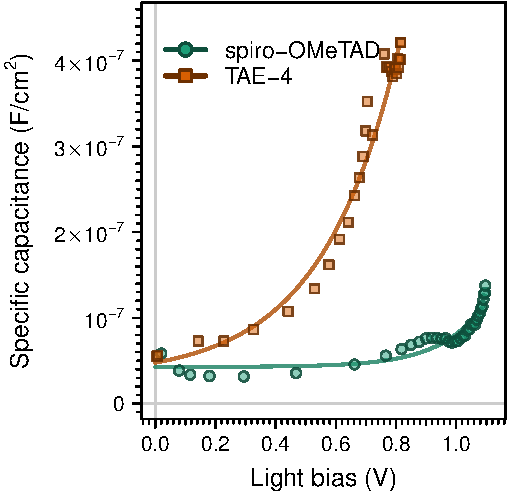
\includegraphics[width=0.75\textwidth]{dc_deltaV/monoexp-spiro_vs_TAEs-DCs-capacitance-crop.pdf}
					\subcaption{Linear factor in an exponential fit}\label{fig:dc_deltaV-monoexp}
				\end{subfigure}
				\bigskip

				\begin{subfigure}[t]{0.5\textwidth}
					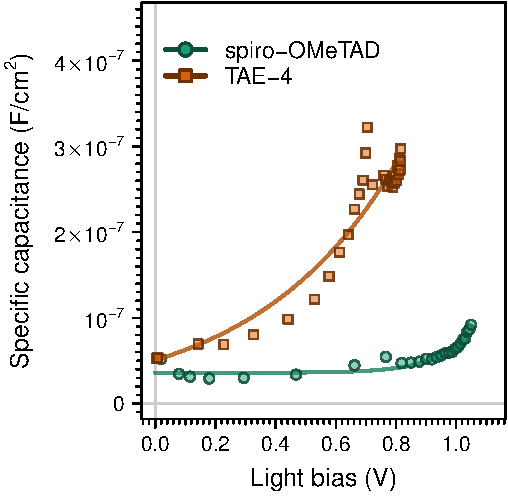
\includegraphics[width=0.75\textwidth]{dc_deltaV/biexp-spiro_vs_TAEs-DCs-capacitance-crop.pdf}
					\subcaption{Sum of linear factors in bi-exp.\ fit}\label{fig:dc_deltaV-biexp}
				\end{subfigure}
				\qquad
				\begin{subfigure}[t]{0.5\textwidth}
					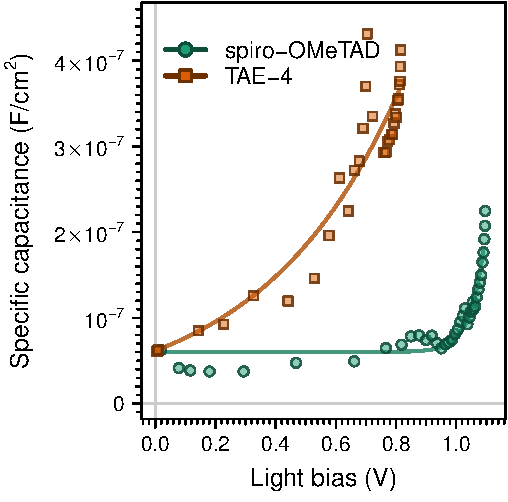
\includegraphics[width=0.75\textwidth]{dc_deltaV/loess-spiro_vs_TAEs-DCs-capacitance-crop.pdf}
					\subcaption{Maximum of a \gls{loess} smoothing}\label{fig:dc_deltaV-loess}
				\end{subfigure}
				\bigskip

				\begin{subfigure}[t]{0.5\textwidth}
					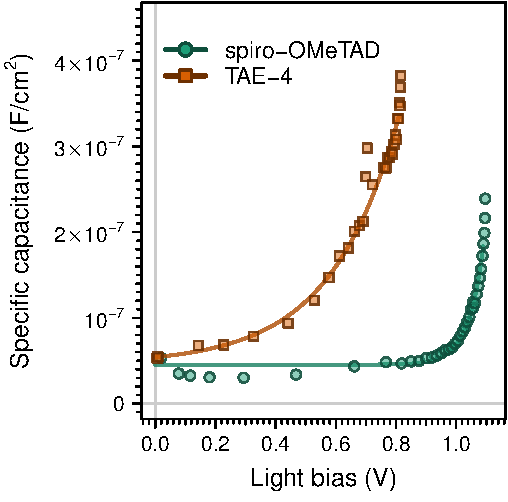
\includegraphics[width=0.75\textwidth]{dc_deltaV/firstPoints-spiro_vs_TAEs-DCs-capacitance-crop.pdf}
					\subcaption{Averaging the peak first points}\label{fig:dc_deltaV-firstPoints}
				\end{subfigure}

				\mycaption[Comparison of methods for obtaining \glsentryshort{dc} experiments.]{
					The capacitance obtained from \acr{dc} experiment on \gls{fto}\-/\ch{d-TiO2}\-/\gls{csfamapbibr}\-/\gls{htm}\-/\ch{Au} devices using different methods for extracting $\Delta V$ value, as detailed in \cpageref{tpv_deltaV}.
				}\label{fig:dc_deltaV}
			}
		}
	\end{figure}

	\paragraph{Capacitance from voltage and current increase during the pulse}
	In case a slow light pulse have to be employed, \textsl{e.g.}\ from a \gls{led} source, the voltage peak is too strongly affected by the ongoing recombination.
	An alternative method considering the plateau current of a \acr{tpc} experiment \textsl{versus} the voltage grow rate from \acr{tpv} has been reported \cite{ORegan2006,ORegan2015b}.

	\paragraph{Comparison of charge from DC and from CE}
	The \acr{dc} experiment has been demonstrated to output a very similar charge \textsl{versus} light bias profile as a \acr{ce} experiment when used on \gls{dssc} \cite{ORegan2005,Barnes2013} and on \gls{osc} \cite{Shuttle2008a}.
	\Acr{dc} started to be employed in perovskite solar cells characterisation due to the excessively large charge amount sometimes measured by \acr{ce} \cite{Wheeler2017,ORegan2015b}.
	Additionally, as explained in \cpageref{characterization_ce_correction}, in cases where high charge recombination is present \acr{ce} should be corrected while \acr{dc} should be unaffected as it can be measured in shorter time scales.
	For obtaining the same parameters as when fitting \acr{ce} data with \cref{eq:ce_full} we can either use that equation for fitting the integrated charge or use the following (which is just the voltage derivative of \cref{eq:ce_full}) for fitting the capacitance:
	\begin{equation}\label{eq:dc_full}
		C_|DC|(V) = C_|g| + \frac{qn_|eq|}{mk_|B|T} \cdot \exp(\frac{qV}{mk_|B|T})
	\end{equation}

	\FloatBarrier
	\newpage
\section{Voltage and Current Reconstruction}
	As a self consistency check for the photophysics techniques explained and for confirming that no important factor has been neglected, the performance parameters of the devices can be reconstructed from the fitted parameters from \acr{tpv}, \acr{ce}, and \acr{dc}.
	The shown \gls{jsc} and \gls{voc} reconstruction methods can be extended to obtain the whole current-voltage sweep \cite{Maurano2011}.

	\paragraph{\Glsentryshort{jsc} reconstruction}\label{jsc_reconstruction}
	The recombination current $J_|rec|$ can be described by the total carriers lifetime (or pseudo first order lifetime) $\tau_|pfo|$ and by the excess charge $n_|CE|$ with the following expression \cite{Wheeler2017,Du2018}: $J_|rec| = n_|CE| / \tau_|pfo|$.
	At open circuit the photo\hyp{}generated current has to match the recombination current (no external current means that these two, at least in steady state conditions, cancel out), so $J_|rec| = J_|ph|$.
	If losses at short circuit are negligible, photo\hyp{}generated current can be approximated by the short circuit current $J_|ph| \approx \jsc$ obtaining \cite{ORegan2015b}:
	\begin{equation}\label{eq:reconstruction_jsc}
		\jsc = \frac{n_|CE|}{\tau_|pfo|}
	\end{equation}

	\paragraph{\Glsentryshort{voc} reconstruction}
	Expanding $\tau_|pfo| = \Phi \tau$ with \cref{eq:tpv_tau_order} and neglecting the intrinsic charge density (consideration valid for non-dark cases) so that $n_0 \approx n_|CE|$ we get:
	\begin{equation}
		\jsc = n_|CE| \cdot k n_|CE|^{\Phi-1}
	\end{equation}
	Then considering just the chemical capacitance\index{chemical capacitance} charge as relevant for recombination processes, so keeping just the exponential addend in \cref{eq:ce_full} we obtain:
	\begin{equation}
		\jsc = n_|eq|^\Phi k \exp(\frac{q \Phi \voc}{m k_|B| T})
	\end{equation}
	again, we neglected $-1$ from the additional intrinsic charge density. Then inverting the equation we obtain:
	\begin{equation}\label{eq:reconstruction_voc}
		\voc = \frac{m k_|B| T}{q \Phi} \ln( \frac{\jsc}{n_|eq|^\Phi k} )
	\end{equation}
	%Expanding \cref{eq:tpv_tau_order} with the relevant $n_0$ for recombination taken from the chemical capacitance\index{chemical capacitance} charge represented by the exponential addend in  we obtain:
	%\begin{equation}\tau_|pfo| = \left\{\Phi k_\Phi n_|eq|^{\Phi-1} [\exp(\frac{q \voc}{m k_|B| T})-1]^{\Phi-1} \right\}^{-1}\end{equation}
	The \cref{eq:reconstruction_voc} now contains just parameters which can be obtained from our photophysical measurements \cite{Wheeler2015,Wheeler2017,Du2018,Barnes2011a}.

\section{Impedance Spectroscopy}\label{characterization_impedance}
	%\epigraph{\textit{"No, I never used this technique, I tried but I couldn't understand it."}}
	\epigraph{\textit{\enquote{One does not simply have a look at impedance spectroscopy data}}}{Boromir}

	\paragraph{Concept}
	Impedance spectroscopy can be performed with easily available equipment: most of the electrochemical units used in the research labs for measuring cyclic voltammetry include this technique.
	An alternated voltage at frequency $\nu = \omega / (2 \pi)$ is applied to the two electrodes of the device and the resulting alternated current is observed in amplitude and phase.
	For an accurate phase estimation usually a lock-in amplifier is used.
	The in-phase component can be taken for calculating a resistance $Z'(\nu)$ and the quadrature component for calculating the reactance $Z''(\nu)$.
	The sum of these two components give the complex impedance: $Z(\nu) = Z'(\nu) + iZ''(\nu)$.
	The voltage oscillation should be large enough for measuring a current profile without too much noise, usually amplitudes from \SIrange{20}{200}{\mV} are employed.
	Repeating this on different alternating voltage frequencies, often from \SIrange{1e-2}{1e7}{\Hz}, the spectra of impedance can be obtained.
	The impedance spectroscopy can be represented in various shapes: Nyquist plots where $-Z''$ is plotted against $Z'$, Bode plots of phase, $|Z|$, $Z''$, or $Z'$ are plotted against the frequency $\nu$ or, as a capacitance (or apparent capacitance, as we will see in \cref{ch:impedance}) defined as $\omega^{-1}\Im(Z^{-1})$.

	\paragraph{Frequency\hyp{}domain}
The frequency\hyp{}domain results should be related to the time\hyp{}domain by the Fourier transform, so from frequency\hyp{}domain techniques we should be able to extract the same information as from time\hyp{}domain techniques, as the aforementioned ones (on this topic, see \cpageref{impedance_fourier}).
Nevertheless, frequency\hyp{}domain techniques are more convenient for observing one by one all the different processes happening in a solar cell device, working at their characteristic frequency.
On the other hand this also implies a much longer measurement, for which the device stability is paramount.

	\paragraph{Stability}
	As the measurement of a complete impedance spectra is very time demanding, the device stability is of paramount importance.
	Moreover, degradation processes or stabilisation happening within the studied $1/\nu$ time span (between hundreds of seconds and microseconds) will result in glitches which can be easily mistaken for interesting data \cite{Jacobs2018,Moia2019}.

	\paragraph{Interpretation}
	Due to the large amount of extracted data and the complex features usually observed when studying perovskite solar cells (\textsl{e.g.}\ multiple arcs in the Nyquist plot), the parameters extraction is usually done \textsl{via} fitting with an equivalent electrical circuit.
	A bad choice of the fitting circuit can doom the meaningfulness of the obtained information, so great care has to be taken in order to have a bijective relation between the circuit elements and the relevant physical processes.

	%\section{Stark Spectroscopy (ElectroAbsorbance)}

	%\section{Interpretation of Kelvin Probe Force Microscopy}\label{interpretation_kpfm}

	%\section{Molecular Characterization}
	%	\subsection{Interpretation of Band Gap Values Obtained \textsl{via} Tauc Plot, PhotoLuminescence and Computational Simulations}\label{interpretation_bg}



	%\section{Our Solar Cells Characterization Steps}
	%
	%	In this section I'll describe the routinary characterization performed in Palomares group.


